\documentclass[12pt,a4paper,table]{report}
\usepackage[utf8]{inputenc}

\usepackage{indentfirst}
\usepackage{adjustbox}
\usepackage{xcolor}
\usepackage{fontspec}
\usepackage{graphicx}
\usepackage{hyperref}
\usepackage{array}
\usepackage{multirow}
\usepackage{amsmath}
\usepackage{amssymb}
\usepackage{geometry}

\usepackage{titlesec}
\usepackage{tocloft}
\usepackage{setspace}
\usepackage{pdfpages}
\usepackage{longtable}
\usepackage{colortbl}
\usepackage{tcolorbox}
\usepackage{diagbox}
\usepackage{polyglossia}
\setmainlanguage{english}
\setotherlanguages{french, arabic}




\usepackage{acronym}
% Configure ToC to show sections but not subsections
\setcounter{tocdepth}{1}
% Prevent hyphenation
\hyphenpenalty=10000
\exhyphenpenalty=10000

\setlength{\headheight}{14.5pt}
\addtolength{\topmargin}{-2.5pt}
\setmainfont{Garamond}[
    Extension = .otf,
    Path = ./font/,
    UprightFont = *-Regular,
    BoldFont = *-Bold,
    ItalicFont = *-Italic,
    BoldItalicFont = *-BoldItalic,
]
\newfontfamily\arabicfont[Script=Arabic]{Amiri}
%\setmainfont{Amiri}[
%Extension = .ttf,
%Path = ./font/,
%UprightFont = *-Regular,
%BoldFont = *-Bold,
%ItalicFont = *-Italic,
%BoldItalicFont = *-BoldItalic,
%]

\geometry{
top=2.5cm,
bottom=2.5cm,
left=2.5cm,
right=2cm,
bindingoffset=1cm
}

% Package setup
\titleformat{\chapter}[display]
{\normalfont\LARGE\bfseries\centering}
{}
{20pt}
{}
[\vspace{1em}\titlerule]

\titleformat{\section}[block]
{\normalfont\Large\bfseries}
{\thesection}
{1em}
{}

\titleformat{\subsection}[hang]
{\normalfont\large\bfseries}
{\hspace*{2em}\thesubsection}
{1em}
{}
[\vspace{0.5em}]

\titleformat{\subsubsection}[hang]
{\normalfont\normalsize\bfseries}
{\hspace*{4em}\thesubsubsection}
{1em}
{}
[\vspace{0.5em}]

\renewcommand{\contentsname}{Table of Contents}
\renewcommand{\listfigurename}{List of Figures}
\renewcommand{\listtablename}{List of Tables}
\renewcommand{\scdefault}{sc}
\renewcommand{\bfdefault}{b}
%%

%%
\onehalfspacing
\usepackage{fancyhdr}
\usepackage{lastpage} % For getting last page number
% Headers and footers
% Headers and footers
\pagestyle{fancy}
\fancyhf{}
\lhead{ISET of Zaghouan}
\rhead{June 2024}
\lfoot{Ouchari Ibrahim}
\rfoot{Page \thepage\ }
\renewcommand{\headrulewidth}{0pt}
\renewcommand{\headrulewidth}{1pt}
% Command to display chapter content summary
% Define a tcolorbox style for the plan
\tcbset{
mybox/.style={
colframe=black,
colback=white,
sharp corners,
boxrule=0.5mm,
width=\textwidth,
center title
}
}

%================= Defining Custom Colors =================%
\usepackage{enumerate}
\usepackage{enumitem}
\usepackage{datatool}% http://ctan.org/pkg/datatool
\newcommand{\sortitem}[2][\relax]{%
\DTLnewrow{list}% Create a new entry
\DTLnewdbentry{list}{sortlabel}{#1}
\DTLnewdbentry{list}{description}{
\begin{minipage}[l]{0.1\columnwidth}
~\textbf{#1}
\end{minipage}
\begin{minipage}[l]{0.05\columnwidth}
\textbf{=}
\end{minipage}
\begin{minipage}[l]{0.85\columnwidth}
#2
\end{minipage}
}% Add entry description
}
\newenvironment{acronyms}{%
\DTLifdbexists{list}{\DTLcleardb{list}}{\DTLnewdb{list}}% Create new/discard old list
}{%
\DTLsort{sortlabel}{list}% Sort list
\begin{itemize}%
\DTLforeach*{list}{\theDesc=description}{%
\item \theDesc}% Print each item
\end{itemize}%
}

%================= configuring minitoc ==================%
\usepackage[english]{minitoc}
\mtcsettitle{minitoc}{Plan}
\setcounter{minitocdepth}{1}

\mtcsetoffset{minitoc}{-1.0em}

%=============== Customizing Chapters Names ===============%

\makeatletter
\def\thickhrulefill{\leavevmode \leaders \hrule height 1.2ex \hfill \kern \z@}

\def\@makechapterhead#1{%
    \vspace*{30\p@}%
    {\parindent \z@ \centering \reset@font
    \thickhrulefill\quad
    \scshape\bfseries\textit{\@chapapp{} \thechapter}
    \quad \thickhrulefill
    \par\nobreak
    \vspace*{10\p@}%
    \interlinepenalty\@M
    \hrule
    \vspace*{10\p@}%
    \Huge \bfseries #1 \par\nobreak
    \par
    \vspace*{10\p@}%
    \hrule
    \vskip 50\p@
    }
}

\def\@makeschapterhead#1{%
    \hbox{\huge\textbf{#1}}%
    \par\vskip 1cm
}
\makeatother
%%%%%%%%%%%%

%%%%%%%%%%%
\usepackage{csquotes}
\PassOptionsToPackage{%
backend=biber, %instead of bibtex
%backend=bibtex8,bibencoding=ascii,%
%language=autobib,%
language=auto,
%language=french,
%autocite=inline,
%style=numeric-comp,%
%style=authoryear-comp, % Author 1999, 2010
%style=authoryear,%
%style=alphabetic,%
style=ieee,
%bibstyle=authoryear,dashed=false, % dashed: substitute rep. author with ---
%sorting=nty, % name, year, title
sorting=none, % name, year, title
%maxbibnames=3, % default: 3, et al.
%backref=true,%
%hyperref=true,
%natbib=true % natbib compatibility mode (\citep and \citet still work)
}{biblatex}

%\renewcommand*{\bibfont}{\small\raggedright}
%\DefineBibliographyExtras{french}{\renewcommand*\mkbibnamelast[1]{#1}}

\usepackage[backend=biber, style=numeric]{biblatex}
\addbibresource{biblio.bib}
\DefineBibliographyStrings{english}{%
bibliography = {Webography},
}
\usepackage{changepage} % For the adjustwidth environment

% % Redefine section and subsection with titlesec
% \titleformat{\section}
% {\normalfont\Large\bfseries}{\thesection}{1em}{}
% \titlespacing*{\section}{0pt}{\baselineskip}{\baselineskip}

% \titleformat{\subsection}
% {\normalfont\large\bfseries}{\thesubsection}{1em}{}
% \titlespacing*{\subsection}{0pt}{\baselineskip}{\baselineskip}

% % Redefine \section and \subsection to indent the following paragraph
% \let\oldsection\section
% \renewcommand{\section}[1]{\oldsection{#1}\par\hspace{1.5em}}
% \let\oldsubsection\subsection
% \renewcommand{\subsection}[1]{\oldsubsection{#1}\par\hspace{2.5em}}

% Redefine section and subsection with titlesec
% Redefine \section and \subsection to indent the following paragraph
% Redefine \section and \subsection to indent the following paragraph

% Redefine section and subsection with titlesec
% \titleformat{\section}
% {\normalfont\Large\bfseries}{\thesection}{1em}{}
% \titlespacing*{\section}{0pt}{\baselineskip}{\baselineskip}

% \titleformat{\subsection}
% {\normalfont\large\bfseries}{\thesubsection}{1em}{}
% \titlespacing*{\subsection}{0pt}{\baselineskip}{\baselineskip}

% \let\oldsection\section
% \renewcommand{\section}[1]{%
% \ifx*#1%
% \oldsection*{#1}\addcontentsline{toc}{section}{#1}\par%
% \else%
% \oldsection{#1}\addcontentsline{toc}{section}{\protect\numberline{\thesection}#1}\par\hspace{1.5em}%
% \fi%
% }
% \let\oldsubsection\subsection
% \renewcommand{\subsection}[1]{%
% \ifx*#1%
% \oldsubsection*{#1}\addcontentsline{toc}{subsection}{#1}\par%
% \else%
% \oldsubsection{#1}\addcontentsline{toc}{subsection}{\protect\numberline{\thesubsection}#1}\par\hspace{2.5em}%
% \fi%
% }



\begin{document}

% Set the counters to start from 1
\setcounter{chapter}{0}
\setcounter{section}{0}
\setcounter{subsection}{0}
\setcounter{subsubsection}{0}
\pagenumbering{gobble}
% Include PDF as the first page
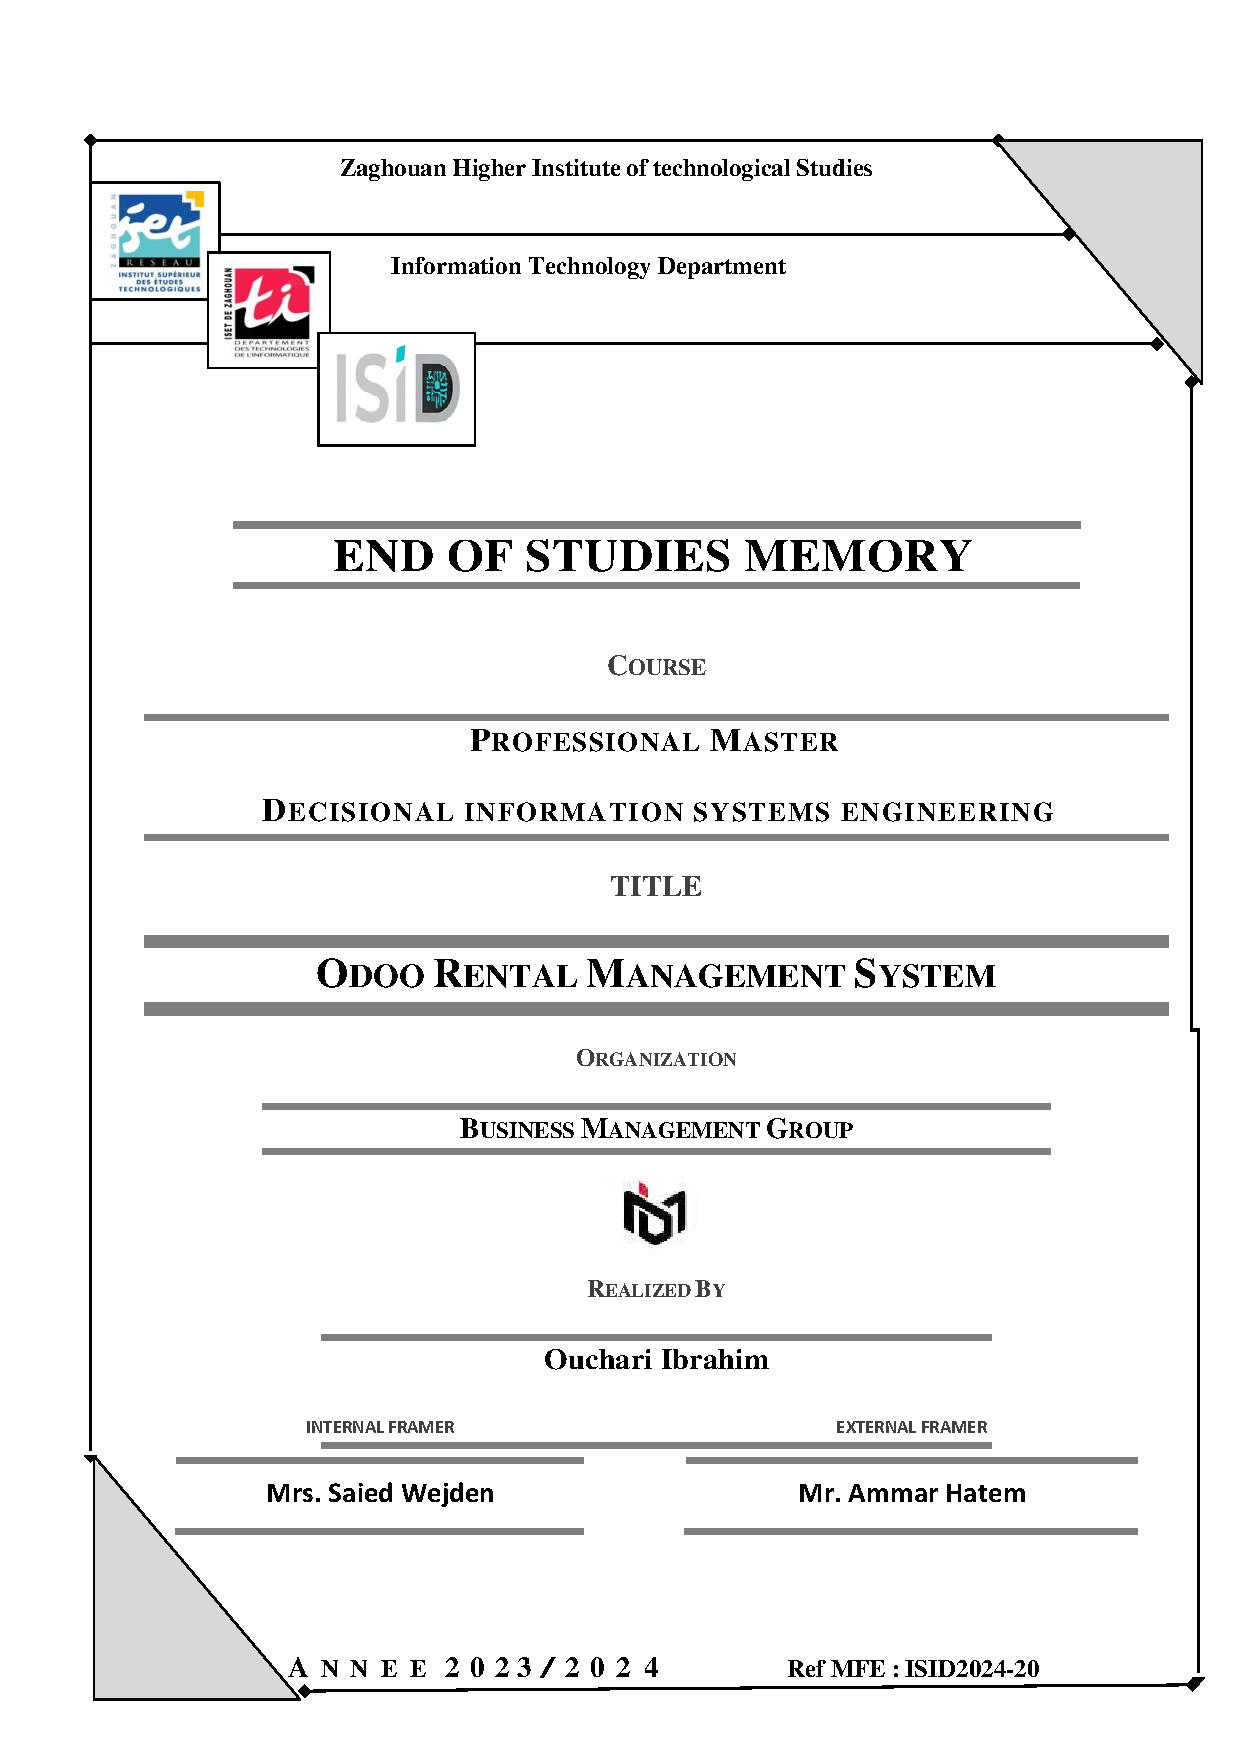
\includepdf[pages={1}]{media/page_guard.pdf}
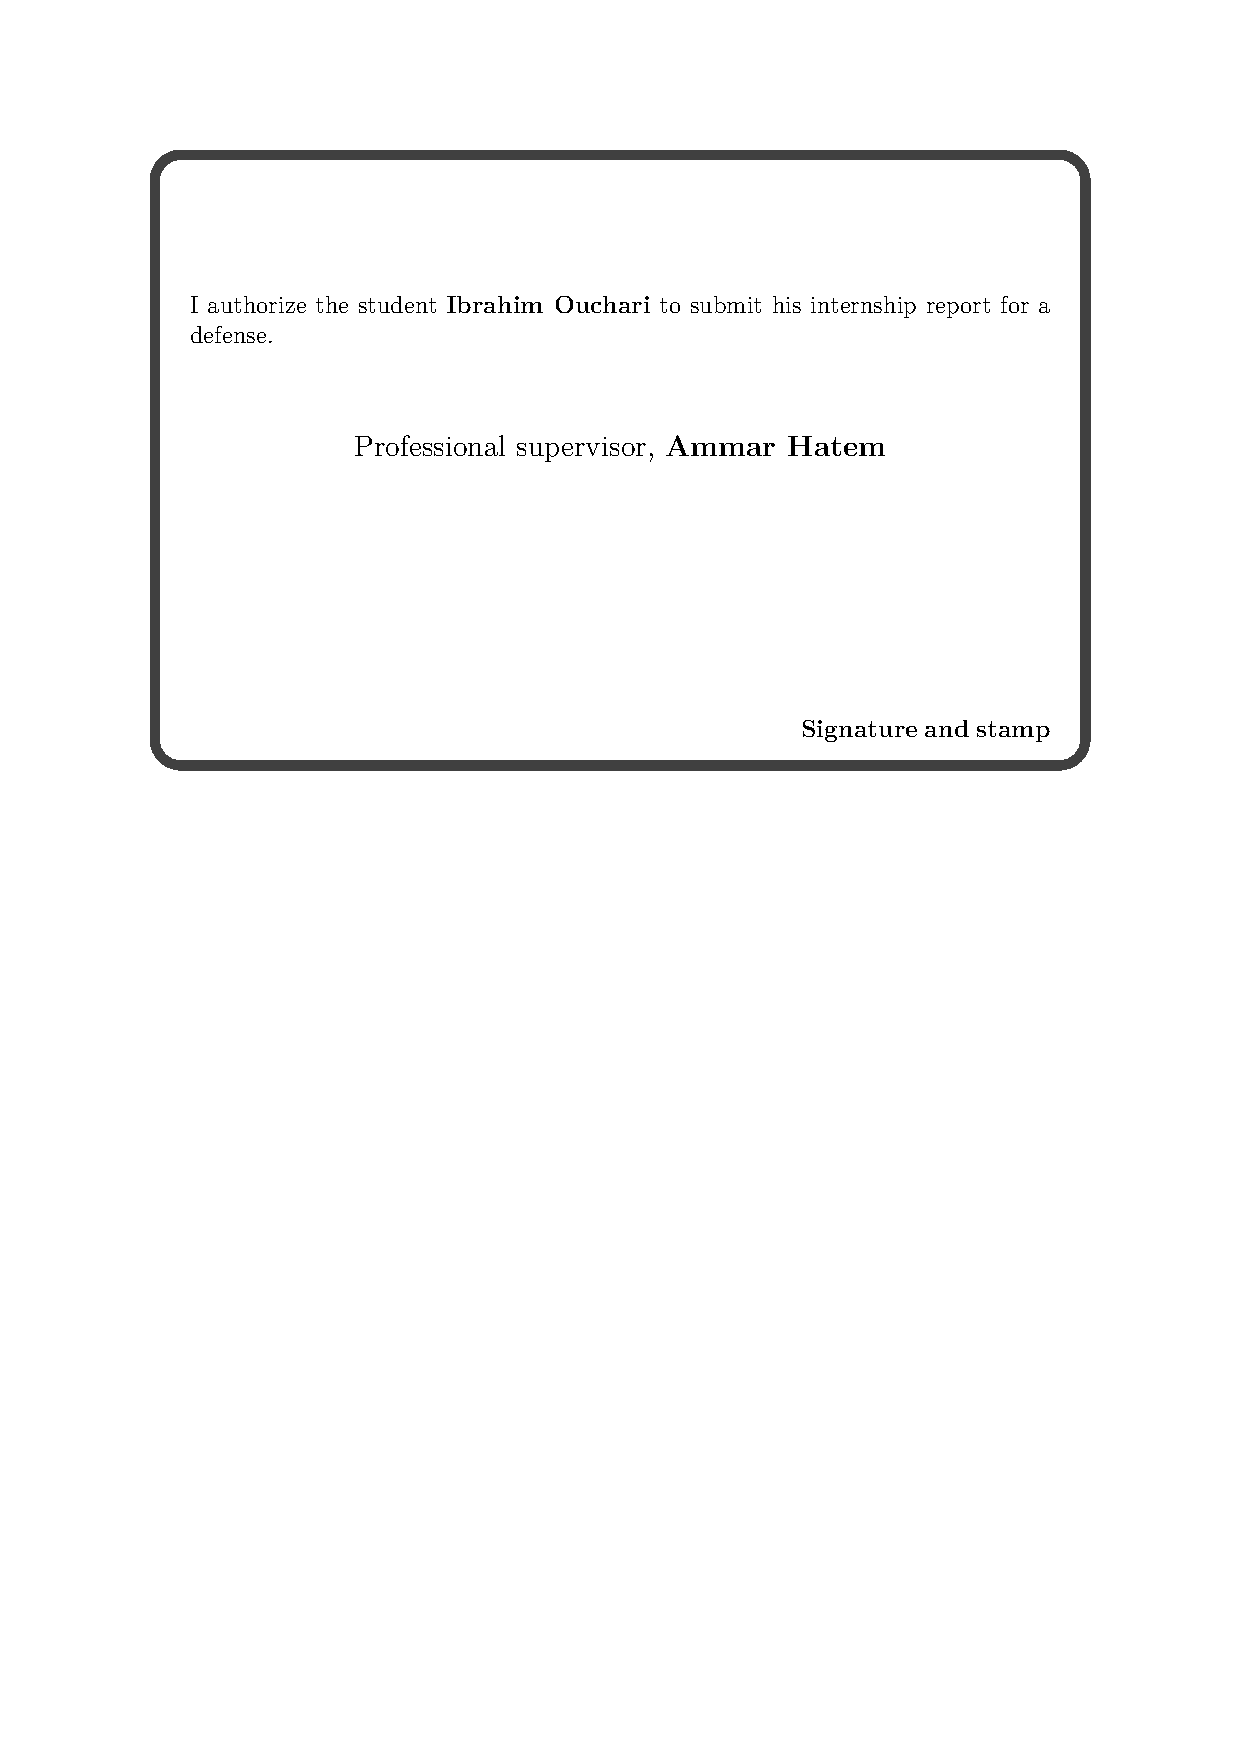
\includepdf[pages={1}]{media/signatures.pdf}
\setcounter{page}{1}
% Cover Page
\chapter*{\centering \LARGE Dedication}

\vspace{1cm}
Dedications
I dedicate this work :

To my dear mother Mouna, the most tender of women, who always made
sacrifices to ensure I had a healthy and wonderful life. Your encouragement and love were
always my guiding light. I hope I have lived up to the hopes you had for me and fulfilled one
of your dreams today.

To my brothers Ahmed, Radhouene and Omar for the times of happiness and companionship we have
experienced together. Your presence and constant support have given me solace during
moments of uncertainty. You have not only been my brothers but also a My Rock, and I
value all the enjoyable moments and your affectionate brotherly love.
To my Mariem and my aunt Nabila, you were the second mom and sisters figuers for me my entire life. and for that person who without him I wouldn't be able to get throught this far I am truly grateful for everything you have done for
me. Your unwavering support is my greatest source of motivation, and I appreciate having
you by my side.
With love and gratitude,
Ouchari Ibrahim

\vspace{1cm}

\noindent \large Ouchari Ibrahim
\thispagestyle{empty}
\chapter*{\centering \LARGE Acknowledgments}

\vspace{1cm}

I also want to express my gratitude and appreciation to \textbf{Mm. Wejden Saied} and my manager \textbf{Mr. Hatem AMMAR}.

By accepting to lead this end-of-studies project, despite your numerous responsibilities, you have bestowed your trust upon me. Your open-mindedness and, above all, your interest in science make you an endless source from which every student should drink.

I would like to particularly thank the members of the jury for agreeing to evaluate this dissertation. May they find in this work the expression of my respect and sincere gratitude.

I would like to express my gratitude to my family, friends, and colleagues who have provided me with their moral and intellectual support throughout this work.

To all those who have contributed to the completion of this work, whether directly or indirectly, please accept my heartfelt recognition and thanks.
\vspace{1cm}
\thispagestyle{empty}

\newpage
\dominitoc
\tableofcontents
\thispagestyle{empty}
\newpage
\listoftables
\thispagestyle{empty}
\newpage
\listoffigures
\thispagestyle{empty}
\newpage
\chapter*{List of Acronyms}

\begin{acronyms}
    \sortitem[ERP]{
        \textbf{E}nterprise \textbf{R}esource \textbf{P}lanning
    }
    \sortitem[CRM]{
        \textbf{C}ustomer \textbf{R}elationship \textbf{M}anagement
    }
 
    \sortitem[UML]{
        \textbf{U}nified \textbf{M}odeling \textbf{L}anguage
    }
    \sortitem[GUI]{
        \textbf{G}raphical \textbf{U}ser \textbf{I}nterface
    }
    \sortitem[PDF]{
        \textbf{P}ortable \textbf{D}ocument \textbf{F}ormat
    }
    \sortitem[SQL]{
        \textbf{S}tructured \textbf{Q}uery \textbf{L}anguage
    }
    \sortitem[XML]{
        \textbf{X}tensible \textbf{M}arkup \textbf{L}anguage
    }
    \sortitem[MVC]{
        \textbf{M}odel-\textbf{V}iew-\textbf{C}ontroller
    }
    \sortitem[ORM]{
        \textbf{O}bject \textbf{R}elational \textbf{M}apping
    }
    \sortitem[CSS]{
        \textbf{C}ascading \textbf{S}tyle \textbf{S}heets
    }
  
    \sortitem[Git]{
        \textbf{G}lobal \textbf{i}nformation \textbf{t}racker
    }
   
\end{acronyms}

\thispagestyle{empty}

\chapter*{\centering General Introduction}

\pagenumbering{arabic} % Start page numbering from here
\addcontentsline{toc}{chapter}{General Introduction}

The project highlights the rapid evolution of the digital landscape, particularly in a post-pandemic era, underscoring the increasing need for digitalization. It focuses on analyzing, designing, and developing an Odoo-based system to address initial project requirements, showcasing technology's pivotal role in modern business operations.

Odoo, renowned for its robust open-source ERP \cite{erp} capabilities, offers versatile solutions tailored for efficient business management across various industries. Its user-friendly interface and flexibility empower businesses of all scales, automating processes to boost productivity and minimize redundancy. Adopting the Scrum methodology ensured effective planning, execution, and stakeholder engagement throughout project phases.

This initiative aimed to leverage Odoo and Scrum methodologies to enhance software development skills and agile \cite{agile} project management expertise. Subsequent chapters outline project achievements, with an introduction and concluding remarks framing the narrative.

This report is structured as follows.

This report details the steps taken to complete the project, divided into five chapters.

Chapter 1 introduces the project's context, including the host organization, the problem statement, and project requirements.

Chapter 2 focuses on the preliminary study and identifies functional and non-functional requirements using the adopted methodology.

Chapters 3 to 5 detail the design and modeling of various application entities.

Chapter 6 covers the tools and environment used to complete the project.

Finally, the report concludes with a summary of the main achievements.

\chapter{GENERAL SCOPE OF THE PROJECT}

\section*{Introduction}
\addcontentsline{toc}{section}{Introduction}
In this chapter, we will begin by defining the project in its practical and theoretical framework. We will present our host organization by detailing its organizational chart and architecture. Subsequently, we will describe the state of the art as well as the problem and limitations of the existing solution. Finally, we will outline the proposed solution.


In this chapter, I will present my project in general terms, setting out the project framework, then looking at the existing situation and the solutions to be provided. Finally, I will present the working methodology adopted for this project.

\section{Project Framework}

I will start by introducing my host organization, which is where my project took place.

\subsection{General presentation of the host organization}

BMG, a consulting firm and publisher of customized and innovative digital solutions, launched in January 2018, whose business is:
\begin{itemize}
    \item Helping customers formalize and implement their digital transformation projects.
    \item Supporting economic players and NGOs in the design and implementation of their digital projects, through a targeted consulting and support approach that takes into account human capital and structures the present and makes it evolve in line with the organization's digital strategy.
\end{itemize}

\subsection{Organization chart}

The following figure illustrates the organizational chart of the host organization, providing a clear representation of its structure and hierarchy.

\begin{figure}[h]
    \centering
    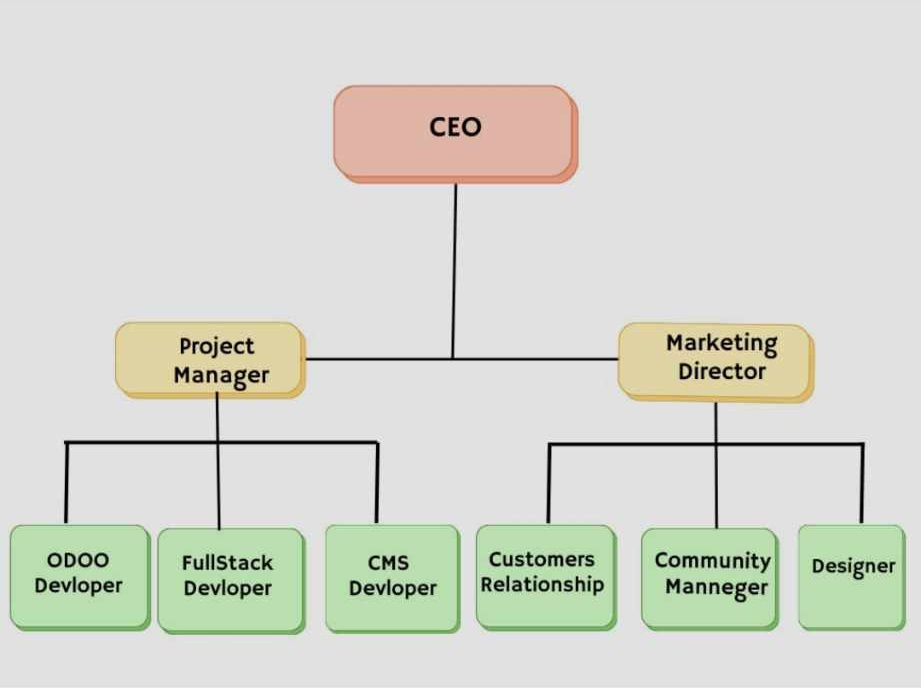
\includegraphics[width=1\textwidth]{media/org.jpg}
    \caption{Organizational chart of the host organization}
    \label{fig:Organizational chart of the host organization}
\end{figure}

\begin{itemize}
    \item Development of collaborative platforms
    \item Mobile development
    \item Web development
    \item E-commerce and marketplaces
    \item SEO and optimization
    \item ERP integration
    \item Data analysis
\end{itemize}


\section{Project Context}

An Enterprise Resource Planning (ERP \cite{erp})  system manages and monitors all information and operational services of a company.

To qualify as an "integrated management software," an ERP must adhere to two fundamental principles:

\begin{itemize}

    \item Building computer applications as independent but compatible modules on a single database.
    \item Using a workflow engine to define tasks and manage their realization across all necessary modules.

    \item Integration: ERP brings together data and processes from different departments into a single platform, avoiding data duplication and facilitating collaboration.

    \item Centralization: ERP provides a real-time overview of the company by centralizing information in a single database, enabling faster and more informed decision-making.
\end{itemize}

In summary, integration and centralization are fundamental ERP principles that optimize company management by unifying information and processes and providing real-time insights.


\subsection{Advantages of Choosing Odoo}

Odoo was selected for its:

\begin{itemize}
    \item Comprehensive Solution: Odoo integrates various business functions like CRM, accounting, and inventory, simplifying management.
    
    \item Flexibility and Customization: Odoo's modular architecture allows easy customization to suit specific needs.
    
    \item Cost-Effectiveness: Odoo's community edition offers competitive pricing with no licensing fees.
    
    \item Strong Community Support: Odoo has a large community of developers and users, providing extensive support and regular updates.
    
    \item User-Friendly Interface: Odoo's clean and intuitive interface enhances user experience, facilitating navigation and feature utilization.
\end{itemize}

\subsection{Advantages of Choosing Odoo for the Project}

Odoo offers several advantages specifically suited to your project needs:

\begin{itemize}
    \item Tailored Solution: Odoo's modular architecture allows for customization to specifically address the requirements of your project, ensuring a tailored solution.
    
    \item Integration Capabilities: With its comprehensive suite of integrated modules, Odoo facilitates seamless integration of various business functions, streamlining project management processes.
    
    \item User-Friendly Interface: Odoo's intuitive interface enhances user experience, enabling smooth navigation and efficient utilization of project management features by your team.
\end{itemize}


\subsection{Project Overview}

Today, companies want to embrace new technologies and use them to be more efficient, hence integrating comprehensive, configurable, and flexible management solutions for handling everything related to their business. This step is crucial to have a clear idea of the existing situation by analyzing it, then formulating an action plan and subsequently conducting a review focusing on weaknesses.

\subsection{Analysis of the Existing System}

The current Odoo rental application exhibits various shortcomings affecting operational efficiency:
\begin{itemize}
    \item Lack of centralized data management leads to data fragmentation and inconsistencies.
    \item Inadequate communication tools result in delays and misunderstandings.
    \item Limited customization options restrict adaptation to unique business needs.
    \item Reporting features are insufficient for real-time insights into operations.
\end{itemize}

\subsection{Critique of the Existing System}

Critiques of the existing Odoo rental app:
\begin{itemize}
    \item Decentralized data storage causes inefficiencies and inaccuracies.
    \item The lack of integrated communication tools leads to coordination issues.
    \item Limited customization hampers adaptation to specific business requirements.
    \item Inadequate reporting capabilities hinder real-time decision-making.
\end{itemize}

\section{Proposed Solution}

Our proposed solution involves the development of a customized rental management system tailored to your specific business needs. This system will offer a user-friendly interface, facilitating seamless control and monitoring of rental operations. By centralizing data management and integrating communication tools, our solution aims to enhance operational efficiency and customer satisfaction.

Key features of our proposed solution include:

\begin{itemize}
    \item Centralized data management to eliminate fragmentation and 
\\ inconsistencies.
    \item Integration of communication tools for improved coordination and client engagement.
    \item Extensive customization options to align the system with your unique business requirements.
    \item Advanced reporting features for real-time insights into rental operations.
\end{itemize}


Before detailing the improvements, the following table \ref{tab:comparison}  provides a comparison between the existing rental Odoo app and the proposed rental Odoo app, highlighting key differences and enhancements.

\begin{table}[h]
\centering
\resizebox{\textwidth}{!}{
\begin{tabular}{|p{3.5cm}|>{\centering\arraybackslash}p{5.5cm}|>{\centering\arraybackslash}p{5.5cm}|}
\hline
\rowcolor{purple!20} \diagbox[dir=NW]{\textbf{Feature}}{\textbf{Systems}} & \textbf{Existing Rental Odoo App} & \textbf{Proposed Rental Odoo App} \\
\hline
\hline
Centralized Data Management & Decentralized data management & Centralized data management eliminates fragmentation and inconsistencies \\
\hline
Communication Tools & Limited communication tools & Integrated communication tools facilitate collaboration \\
\hline
Customization Options & Limited customization options & Extensive customization options for specific requirements \\
\hline
Reporting Features & Insufficient reporting features & Advanced reporting for real-time insights \\
\hline
User Interface & May lack intuitiveness & User-friendly interface for ease of use \\
\hline
Workflow Automation & Minimal workflow automation & Robust workflow automation for process optimization \\
\hline
Scalability & Limited scalability & Scalable architecture for business growth \\
\hline
Customer Support & Limited customer support & Comprehensive customer support for implementation and usage \\
\hline
Integration Capabilities & Limited integration & Seamless integration with other systems \\
\hline
Security & Insufficient security measures & Robust security features for data protection \\
\hline
\end{tabular}
}
\caption{Comparison between Existing and Proposed Rental Odoo Apps}
\label{tab:comparison}
\end{table}
\newpage
\section{Methodology and Modeling Framework Adopted}


The selection of a methodology depends on the project's nature and scale. For small, well-defined projects, a waterfall approach may suffice. However, for projects with evolving requirements, an iterative or prototyping methodology is preferable.

Among iterative methodologies, Agile \cite{agile} methods are widely adopted worldwide. Agile fosters collaboration and embraces incremental approaches, producing high-quality products while accommodating evolving client needs. Agile promotes continuous quality management and early issue detection, minimizing cost and schedule penalties.

The nature of our project, which is evolutionary and characterized by incomplete requirements, led us to adopt an Agile methodology, specifically SCRUM.

\subsection{Overview of SCRUM Methodology}


SCRUM \cite{scrum} methodology emphasizes incremental development through transparent management of evolving requirements. With frequent deliveries, typically every four weeks, clients receive functional software at the end of each iteration. As the project progresses, the software becomes more feature-rich. SCRUM relies on iterative development at a consistent pace to achieve project objectives.


\section{Modeling Language}


As a modeling language, I used the Unified Modeling Language (UML \cite{uml}). It is commonly used in all product projects and offers several diagrams that provide a computational representation of standard elements and real-world problems.


\section*{Conclusion}
\addcontentsline{toc}{section}{Conclusion}

In this chapter, I began by introducing the company, followed by an analysis and critique of the existing system. Based on this assessment, I proposed a solution that aims to address some of the observed issues. Finally, I discussed the choice of modeling language and the methodology adopted.

At this point, I can move on to the next chapter, which will focus on the planning and architecture of the project.

% Set the counters to start from 1


\chapter{ Preliminary Study and Needs Analysis}


\section*{Introduction}
\addcontentsline{toc}{section}{Introduction}

In this chapter, we will provide a clear vision of the project, followed by the creation of our product backlog, and subsequently preparing the production environment.

\section{Needs Framing}

Identifying needs is a crucial step, where different needs and stakeholders will be identified by the end of this phase.

\subsection{Stakeholder Identification}

The stakeholder is an external element to the system demonstrated that interacts directly with it. A stakeholder represents a role played by an external entity (human user, hardware devices, or other systems) that interacts directly with the studied system.

The stakeholders of our application are:
\begin{itemize}
    \item Administrator
    \item Agency Staff
    \item Agency Manager
\end{itemize}

\subsection{Functional Requirements}

Our project aims to automate a set of business processes while working on a single and homogeneous database to increase productivity and reduce redundant work. Thus, each link in the organization will contribute and make it available to other stakeholders in the chain. Therefore, our project is to develop a solution that meets the functional needs of the company:


\begin{itemize}
    \item Product Management: As an administrator, I can add, edit, and delete product information. I can specify if a product can be rented or not.
    \item Rental Order Management: As an administrator, I can manage rental orders, including adding, editing, and deleting orders. As a member, I can view my rental order history.
    \item Stock Management: As an administrator, I can track the picked-up and returned rental quantities of each product to ensure accurate inventory management.
    \item Rental Prices Management: As an administrator, I can set rental prices for each product based on specific periods.
    \item Reservation Management: As a member, I can reserve products for a specific date and time. As an administrator, I can manage and confirm reservations.
    \item Reporting: As an administrator, I can generate various reports, such as sales reports, rental order reports, and inventory reports.
\end{itemize}

\subsection{Non-Functional Requirements}

These are needs that can be perceived by the user and are indirectly related to the system's behavior. The non-functional needs of our system are described as follows:

\begin{itemize}
    \item Performance: Processing time such as functions, calculations, data import/export. Data and report querying, including initial loading time and subsequent loading.
    \item User-Friendliness: Intuitive and user-friendly interface to facilitate system adoption and use by users. Consideration of ergonomics and design for a pleasant user experience.
    \item Extensibility: The application must be extensible, allowing the addition or modification of new features.
    \item \textbf{Security:} Protection of sensitive company and user data. Access rights management to limit unauthorized access to information.


\begin{figure}[htbp]
    \centering
    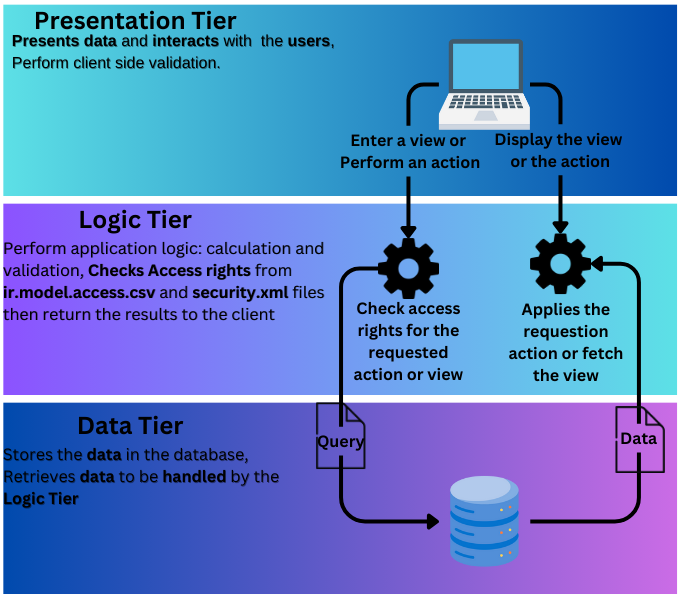
\includegraphics[width=0.9\textwidth]{media/security.png}
    \caption{Access right}
    \label{fig:security}
\end{figure}

\newpage

    \item \textbf{Optimization:} Enhancing the ERP application involves optimizing state management, filtering mechanisms, and implementing efficient Python functions. This ensures streamlined workflows, faster data processing, and improved system responsiveness, thereby enhancing user experience and overall performance.

\begin{figure}[htbp]
    \centering
    \includegraphics[width=1.1\textwidth]{media/optimization.png}
    \caption{Optimization Samples}
    \label{fig:optimization}
\end{figure}

\end{itemize}


\section{Project Breakdown Structure}

We start with the identification of the Scrum team, establishing the "Product Backlog," planning new products, and finally structuring them into "sprints."

\subsection{Scrum Team Identification and Roles}

The development team's primary goal in Scrum is to deliver a deliverable increment at the end of each sprint that maximizes the product's value.

\begin{figure}[h]
    \centering
    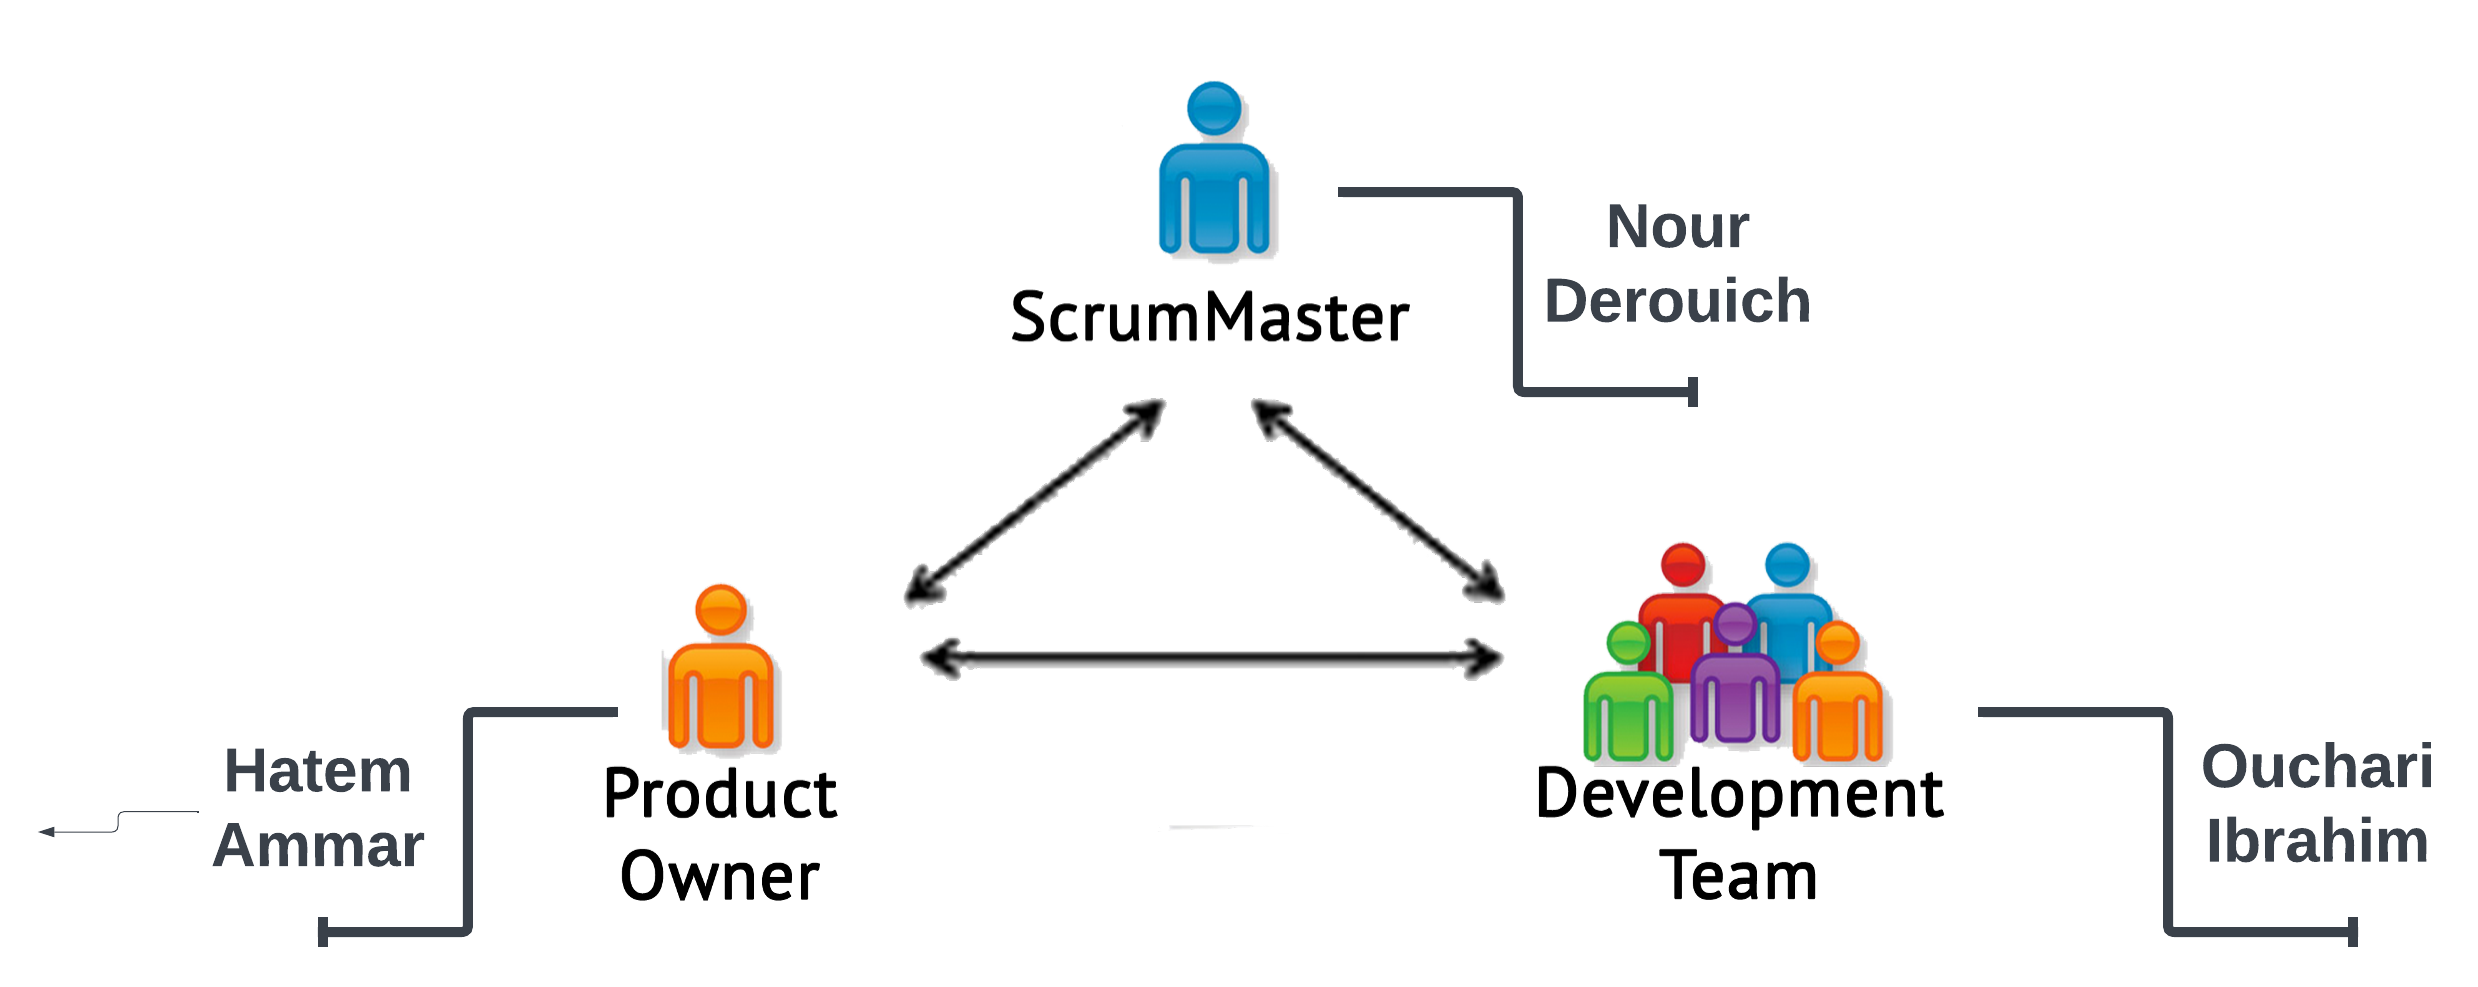
\includegraphics[width=1\textwidth]{media/Scrum_team.png}
    \caption{The actors of a SCRUM project}
    \label{fig:scrum-actors}
\end{figure}
\newpage
\subsection{The Product Backlog}

The Product Backlog is a list of items or features necessary to achieve the objectives or define the expectations within a team, all ranked in order of priority. It allows its members to track their tasks:

\textbf{Importance (Imp):}
The scale of importance ranges from 1 to 5, where 1 indicates less priority and 5 indicates more priority.

\textbf{Complexity (Cmp):}
The complexity scale ranges from + for less complicated, ++ for complicated, to +++ for very complicated. \\
\textbf{Table} \ref{tab:product_backlog} provides a detailed view of the product backlog, including the complexity and importance of each feature.

\begin{longtable}{|c|c|p{5cm}|c|c|}
    \hline
     \rowcolor{purple!20}\textbf{ID} & \textbf{Feature} & \textbf{User Stories} & \textbf{CMP} & \textbf{IMP} \\ \hline
    \endfirsthead
    \hline
     \rowcolor{purple!20}\textbf{ID} & \textbf{Feature} & \textbf{User Stories} & \textbf{CMP} & \textbf{IMP} \\ \hline
    \endhead
    1 & Product Management & 
        \begin{tabular}[t]{@{}p{5cm}@{}}
            - As an administrator, I can manage products in the system. \\
            - As an administrator, I can add new products. \\
            - As an administrator, I can update existing product details. \\
            - As an administrator, I can delete outdated products.\\
            - As an administrator, I can manage periods.\\
            - As an administrator, I can manage the rental pricing.
        \end{tabular}
    & +++ & 5 \\ \hline

  
    2 & Rental Order Management & 
        \begin{tabular}[t]{@{}p{5cm}@{}}
            - As an administrator, I can manage rental orders for products. \\
            - As a member, I can view my rental order history. \\
            - As an administrator, I can generate rental order reports.\\
             - As a member, I can reserve products for a specific date and time. \\
            - As an administrator, I can view and manage product reservations. \\
            - As an administrator, I can confirm or cancel reservations.
        \end{tabular}
    & ++ & 5 \\ \hline
     3 & Stock Management & 
        \begin{tabular}[t]{@{}p{5cm}@{}}
            - As an administrator, I can track stock levels for each product. \\
            - As an administrator, I can receive new stock shipments and update inventory. \\
            - As an administrator, I can set low stock alerts for products.
        \end{tabular}
         
    & ++ & 5 \\ \hline
    4 & Reporting & 
        \begin{tabular}[t]{@{}p{5cm}@{}}
            - As an administrator, I can generate various reports, such as sales reports, rental order reports, and inventory reports. \\
            - As an administrator, I can export reports in different formats (e.g., PDF, Excel).
        \end{tabular}
    & ++ & 4 \\ \hline
    5 & Rental Timeline & 
        \begin{tabular}[t]{@{}p{5cm}@{}}
            - As an administrator, I can view the timeline of product rentals. \\
            - As an administrator, I can track rental durations and return dates.
        \end{tabular}
    & ++ & 4 \\ \hline
    6 & Manage System & 
        \begin{tabular}[t]{@{}p{5cm}@{}}
            - As an administrator, I can configure technical fields of all modules, ensuring that menu configuration is not visible for normal users. \\
            - As an administrator, I can manage users, including creating, updating, and deleting user accounts. \\
            - As an administrator, I can manage access rights for users, specifying their permissions and roles within the system.
        \end{tabular}
    & ++ & 5 \\ \hline
        \caption{Product Backlog with Importance and Complexity}
            \label{tab:product_backlog}\\
\end{longtable}


\section{Global Use Case Diagram}
The Global Use Case Diagram \cite{usecase} provides a comprehensive overview of the system's functional requirements. It visually represents the interactions between various actors and the system, illustrating the different use cases and how users will engage with the system. This diagram is essential for understanding the overall functionality and user interactions within the system.

\begin{figure}[h]
    \centering
    \makebox[\textwidth][c]{%
        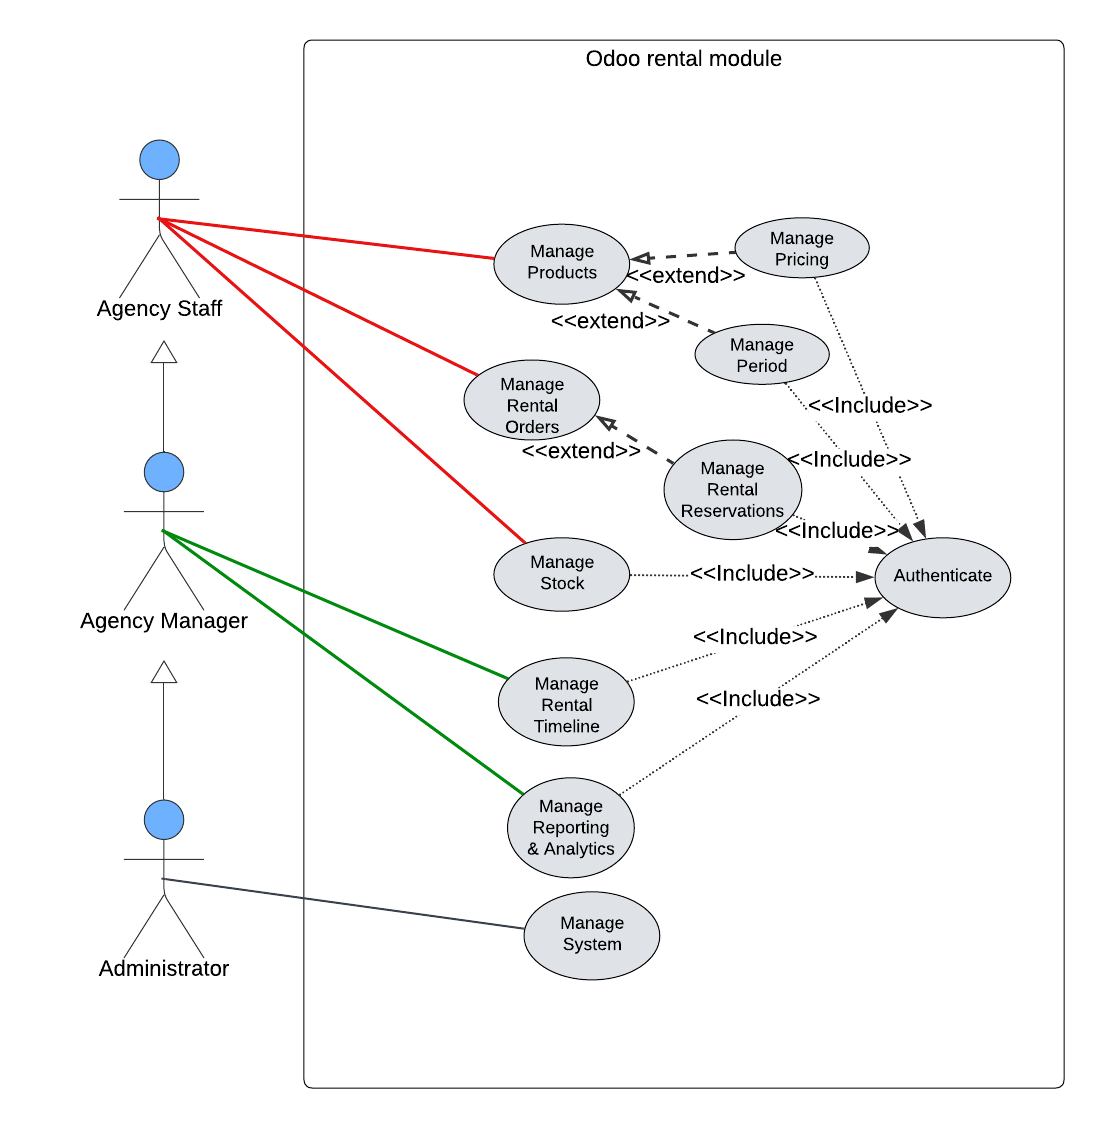
\includegraphics[width=1\textwidth]{media/Use case diagram.png}} % replace with your image path
    \caption{Global Use Case Diagram}
    \label{fig:global-use-case}
\end{figure}

\section{Global Class Diagram}
The Global Class Diagram \cite{classdiagram} depicts the static structure of the system by showing the system's classes, their attributes, methods, and the relationships among objects, serves as a blueprint for constructing the system, providing detailed information on each class's responsibilities and how they collaborate to achieve the desired functionality.

% % Placeholder for the global class diagram
% \begin{figure}[htbp]
%     \centering
%     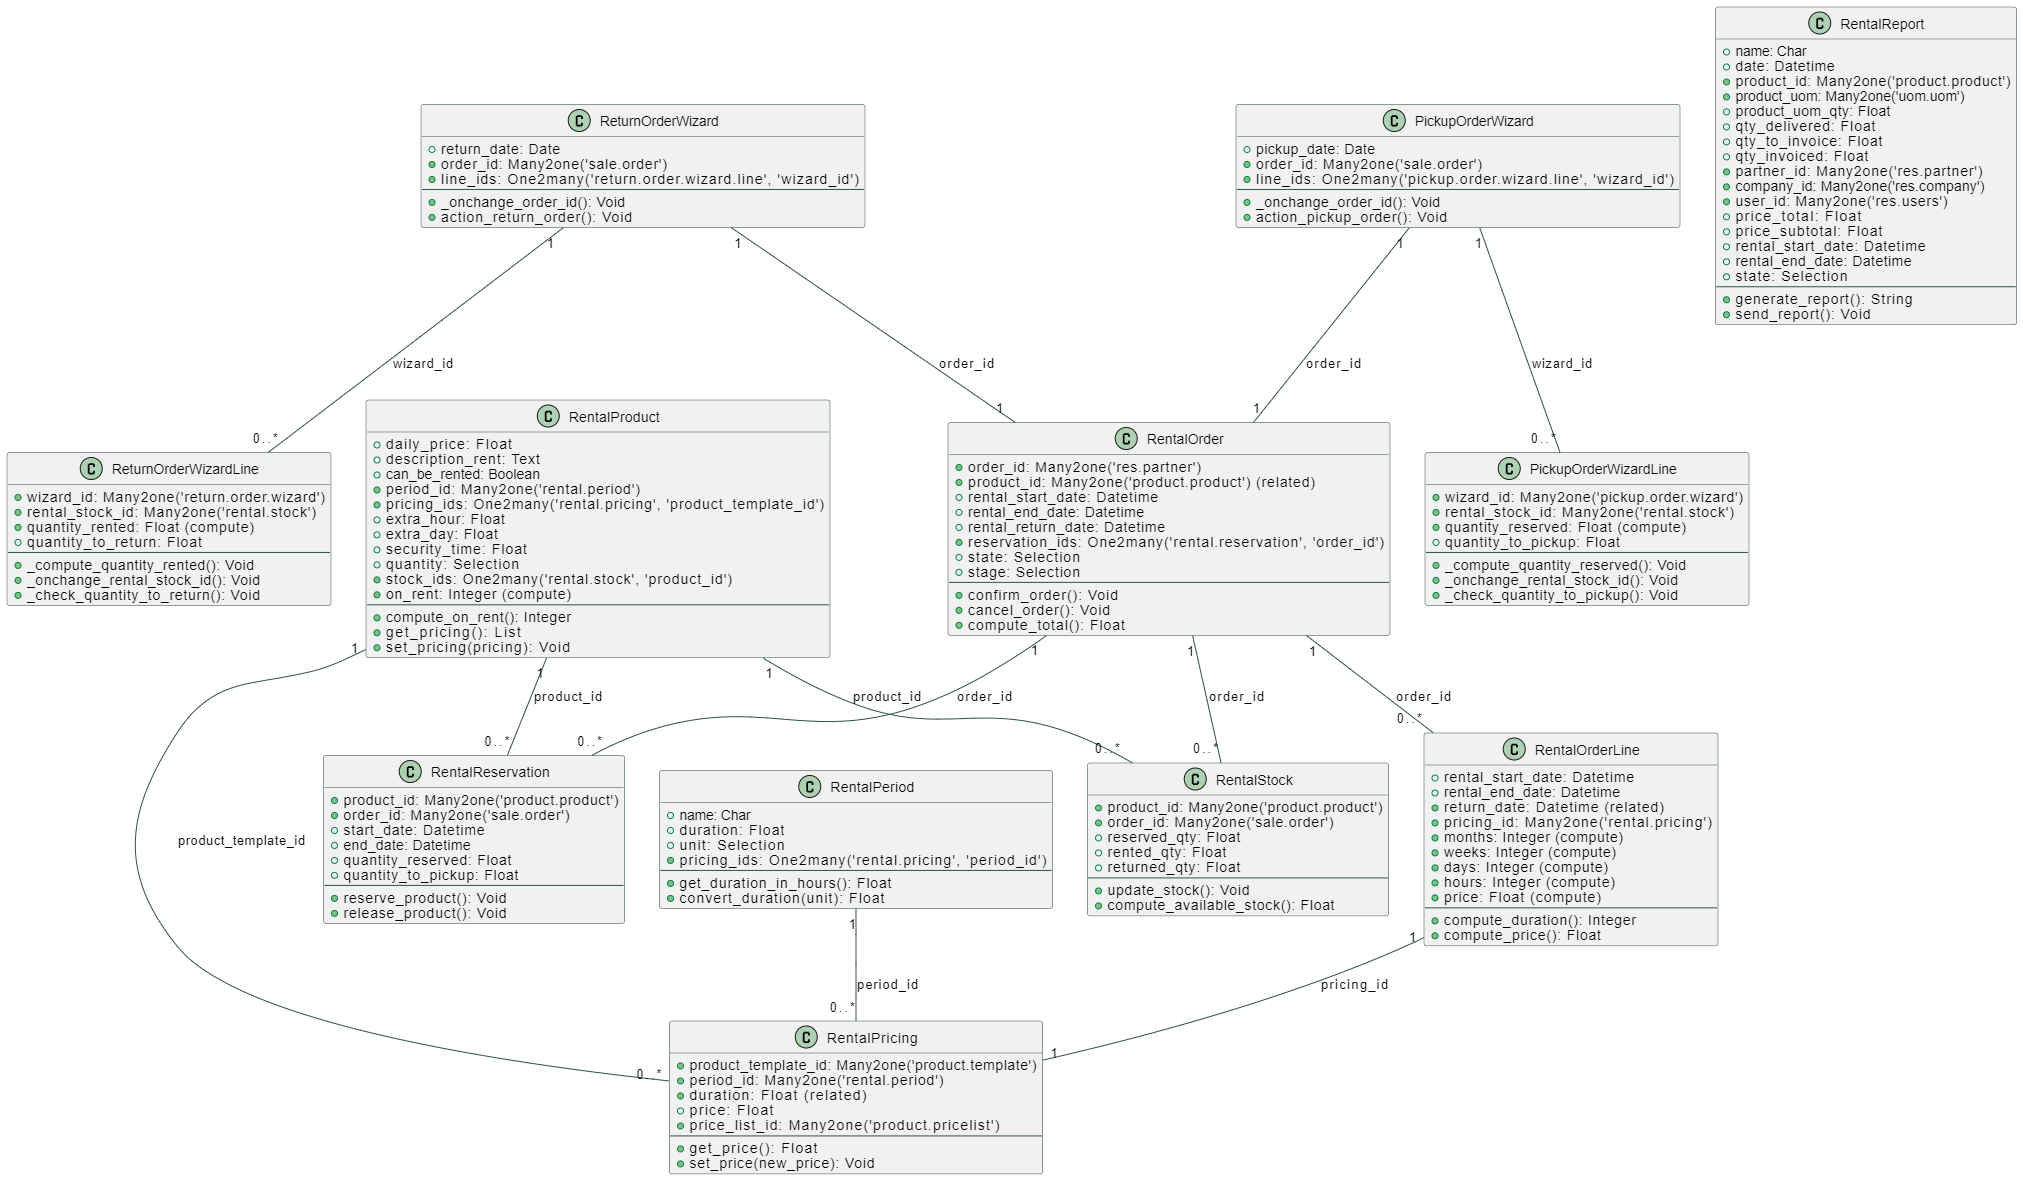
\includegraphics[ width=20cm, angle=90]{media/class_diagram.png}
%     \caption{Global Class Diagram}
%     \label{fig:global-class}
% \end{figure}

\begin{figure}[htbp]
    \centering
    \makebox[\textwidth][c]{%
        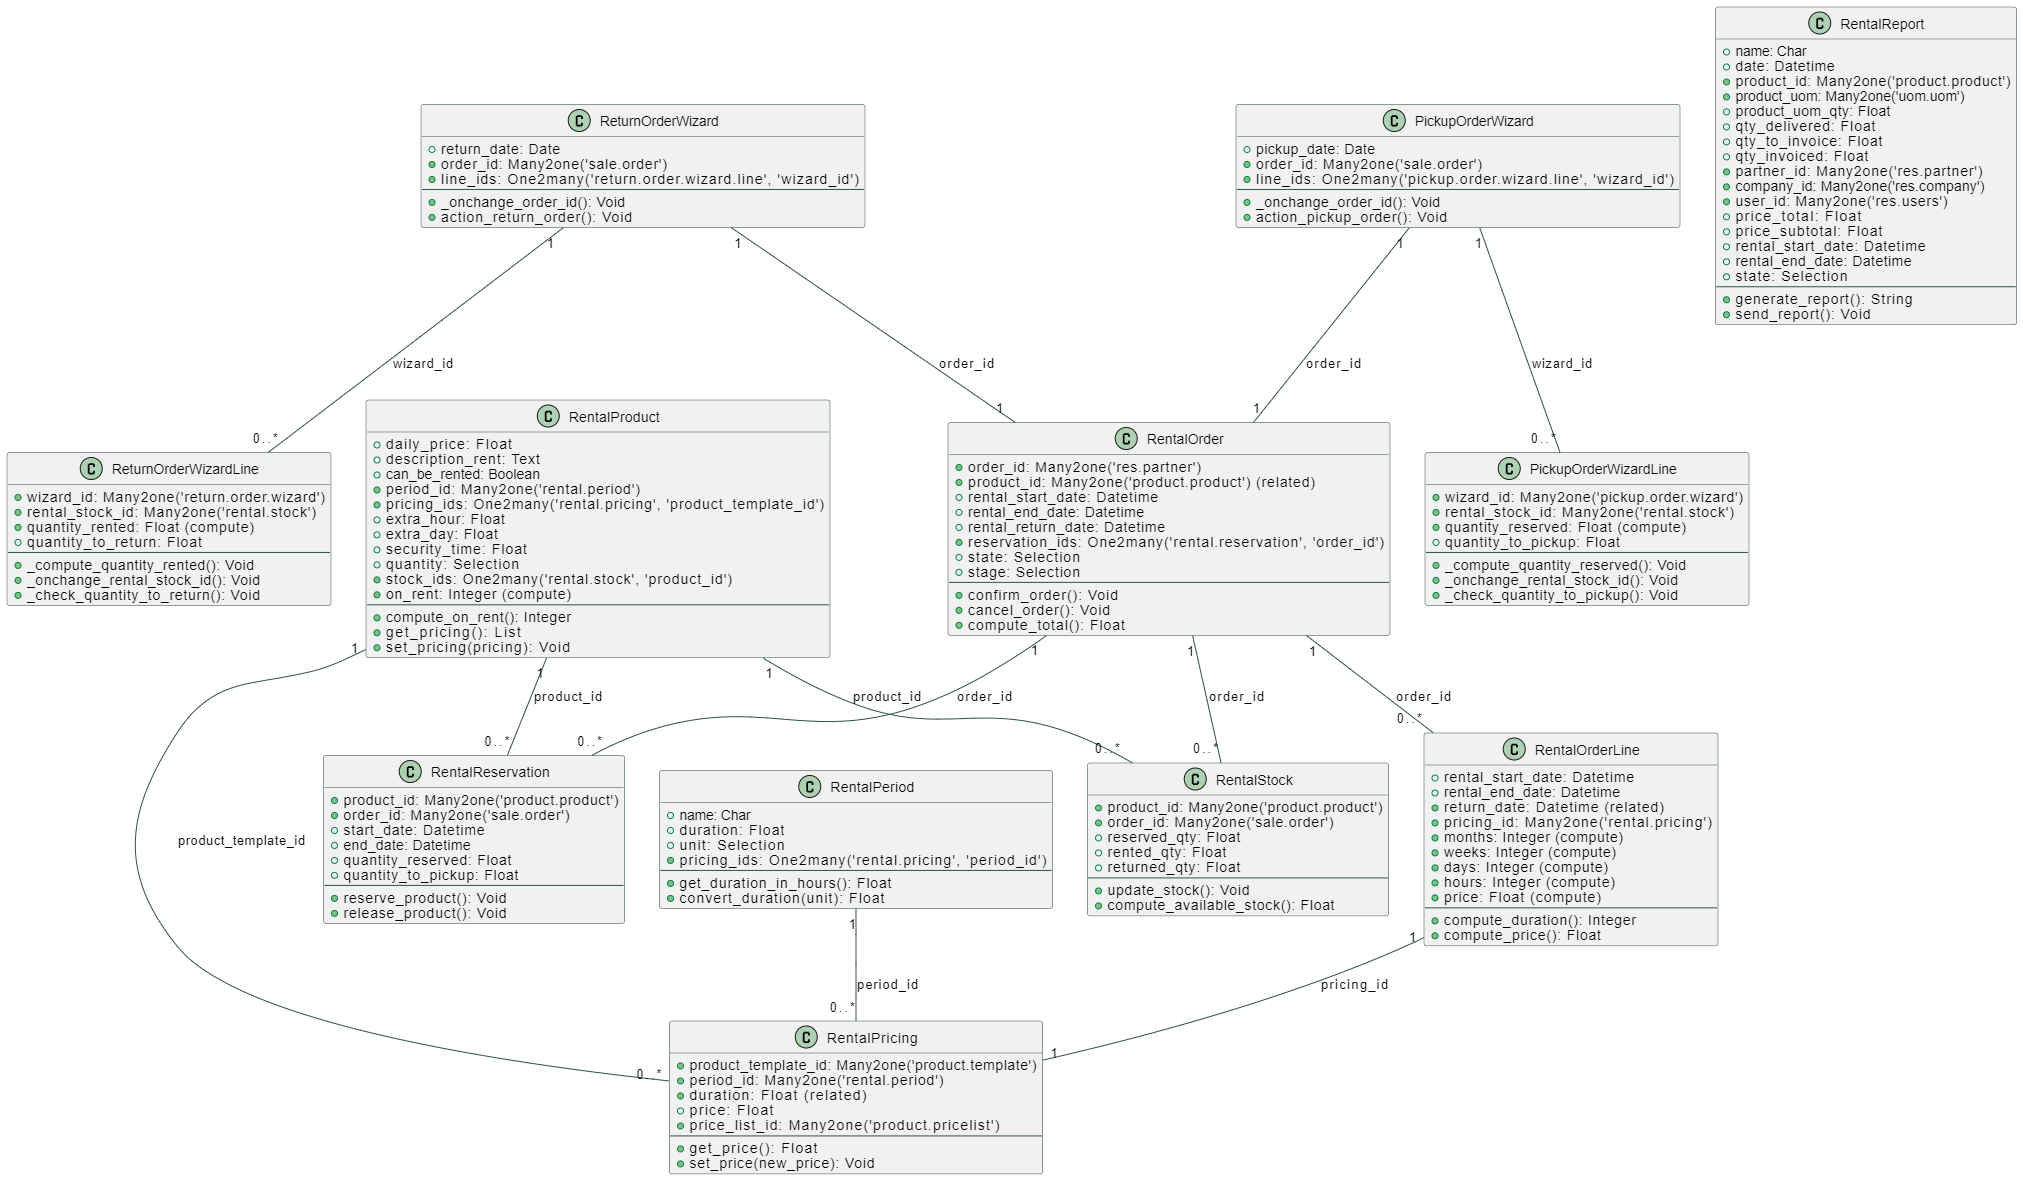
\includegraphics[width=1.6\textwidth, angle=90]{media/class_diagram.png}} % replace with your image path
    \caption{Global Class Diagram}
    \label{fig:global-class}
\end{figure}
\newpage

\section*{Conclusion}
\addcontentsline{toc}{section}{Conclusion}

During this chapter, we have carried out the planning that we intend to follow in our project. We have also identified the actors, the Scrum team, and derived the product backlog from the functional and non-functional requirements captured. Then, we have developed sprint planning as well as the implementation schedule, and established a global use case diagram and a global class diagram.

In the next chapter, we will start our first sprint, and at the end of it, we will have our potentially deliverable first version.
\chapter{Sprint 1 - Design and implementation}

\section*{Introduction}
\addcontentsline{toc}{section}{Introduction}
Previously, we detailed ERP Odoo and our project's progress. Now, we focus on Sprint 1, outlining its key objectives and functionalities.


\section{Sprint 1 Backlog}
The Sprint 1 Backlog lists product management tasks with their estimated durations for efficient planning.

Table \ref{tab:sprint1_product_management} details these tasks and durations..


\begin{longtable}{|c|p{8cm}|c|}
    \hline
    \rowcolor{purple!20} \textbf{N°} & \textbf{Tasks} & \textbf{Duration} \\ \hline
    \endfirsthead
    \hline
    \rowcolor{purple!20} \textbf{N°} & \textbf{Tasks} & \textbf{Duration} \\ \hline
    \endhead
    1 & - As an administrator, I can manage products in the system. & 7 Days \\ \hline
    2 & - As an administrator, I can add new products. & 2 Day \\ \hline
    3 & - As an administrator, I can update existing product details. & 2 Days \\ \hline
    4 & - As an administrator, I can delete outdated products. & 2 Day \\ \hline
    5 & - As an administrator, I can manage periods. & 6 Days \\ \hline
    6 & - As an administrator, I can manage the rental pricing. & 4 Days \\ \hline
    \caption{Sprint 1 Backlog for Product Management}
    \label{tab:sprint1_product_management}
\end{longtable}

\section{Functional Specifications}

\subsection{Use Case Diagram}

In this section, we present the functional specifications for the Product Management module.\\

\begin{figure}[h]
    \centering
    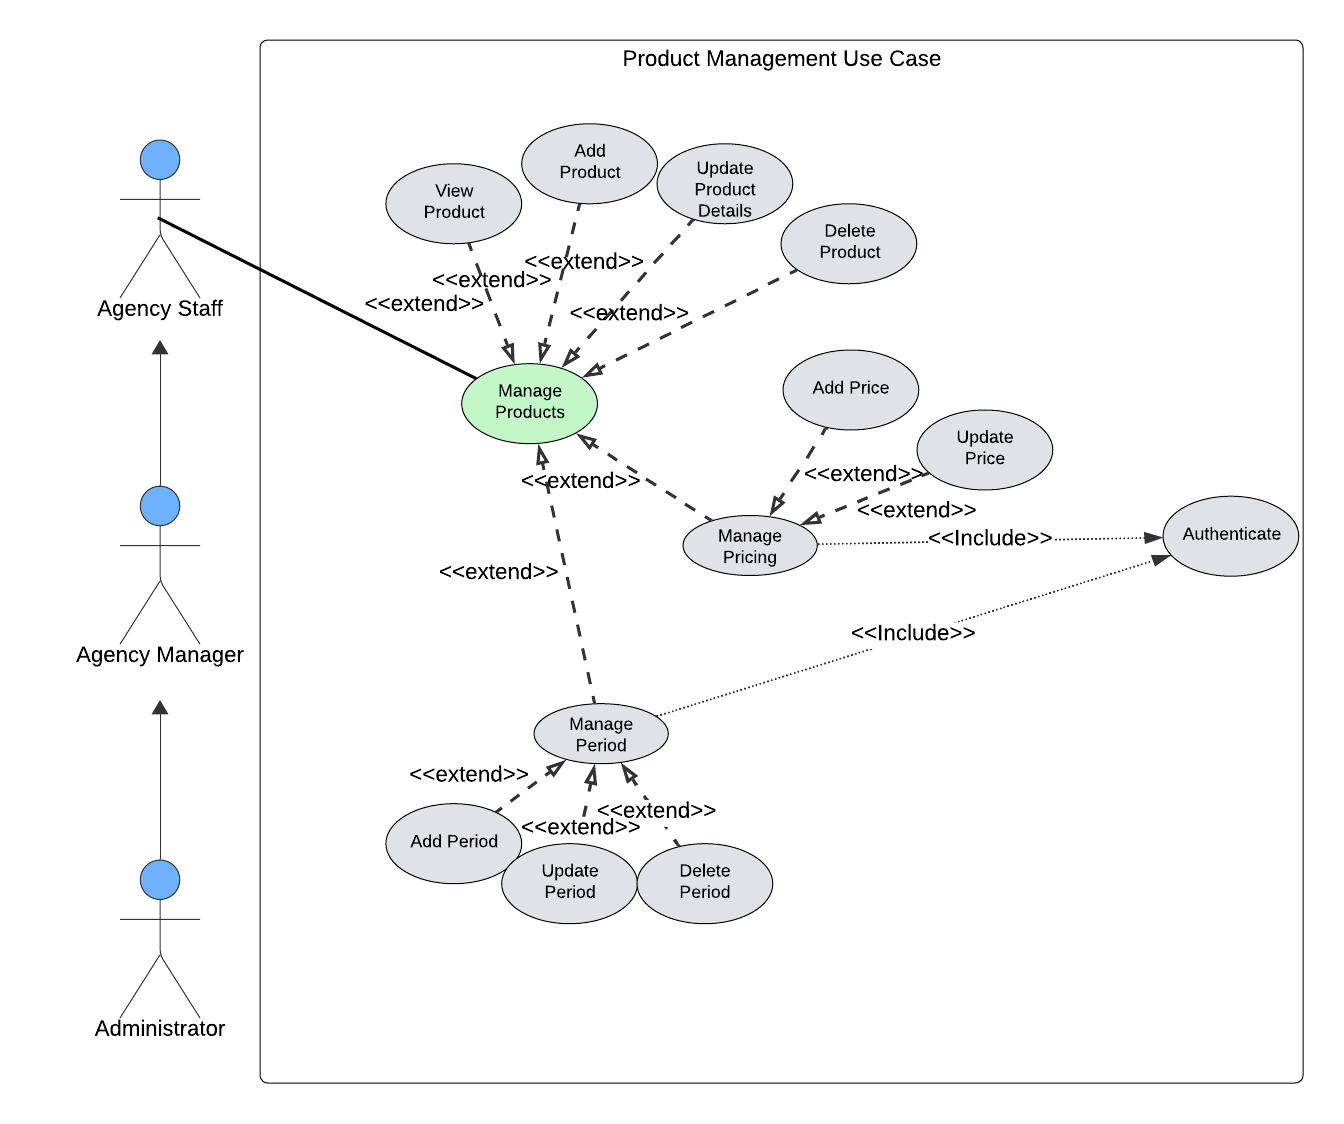
\includegraphics[width=1\textwidth]{sprint1/sprint1usecase.png}
    \caption{Sequence Diagram for "Product Management"}
    \label{fig:product_management_use_case}
\end{figure}

\subsection{Sequence Diagram}
The Sequence Diagram \cite{sequencediagram} illustrates how objects interact to add a new product in Sprint 1, detailing message exchanges and data flow.

\begin{itemize}
    \item Administrator requests new product creation, triggering a form.
    \item Administrator submits form, system verifies data.
    \item Valid data prompts addition to database.
    \item System confirms and displays read-mode form.
    \item Invalid data keeps form in read mode for corrections.
\end{itemize}

\begin{figure}[h]
    \centering
    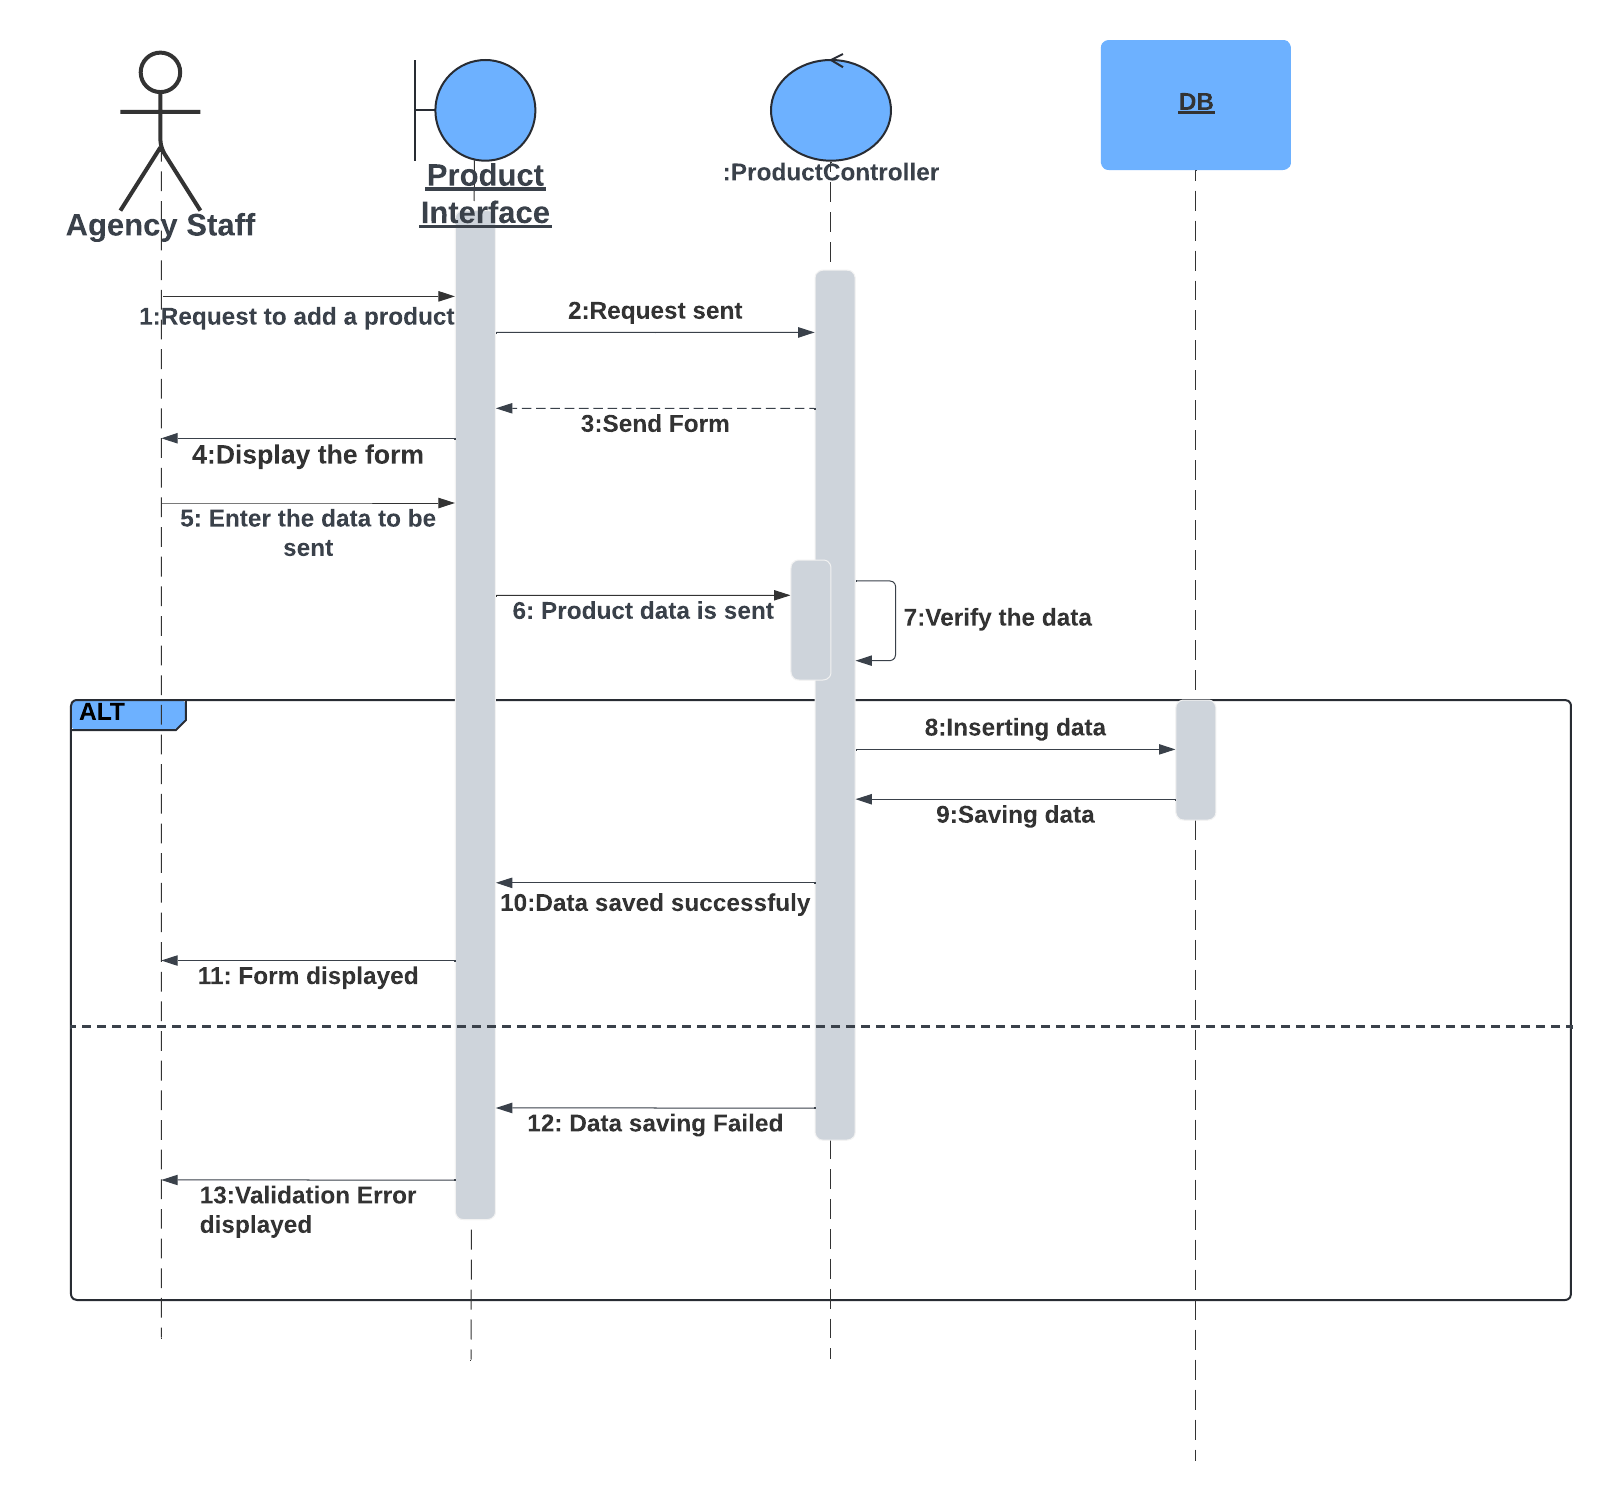
\includegraphics[width=0.9\textwidth]{sprint1/Sprint1Sequence.png}
    \caption{Sequence Diagram for "Product Management"}
    \label{fig:product_management_sequence_diagram}
\end{figure}
\newpage
\section{Sprint Realization}

\subsection{Login Process for Agency Staff in Odoo}
\begin{itemize}
    \item Agency staff authenticate by entering their credentials.
    \item System verifies submitted username and password.
    \item Valid credentials grant access; invalid ones prompt re-entry.
\end{itemize}

\begin{figure}[h]
    \centering
    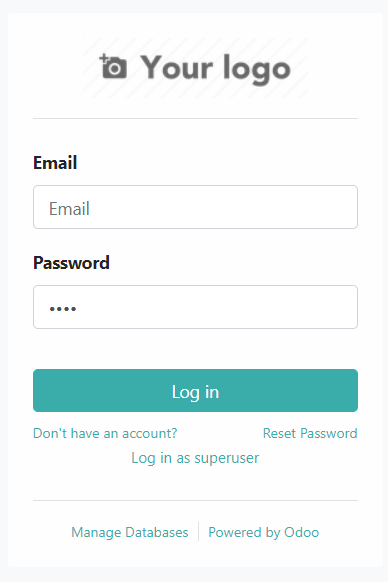
\includegraphics[width=0.45\textwidth]{sprint1/login.png}
    \hfill
    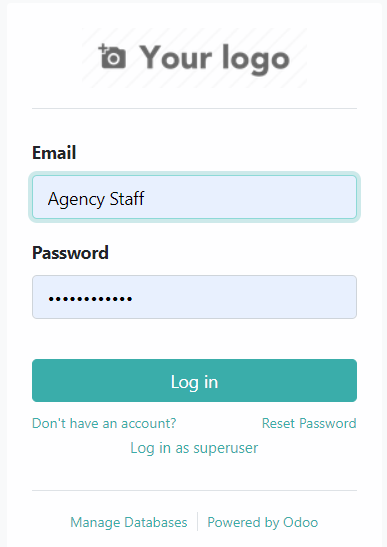
\includegraphics[width=0.45\textwidth]{sprint1/login2.png}
    \caption{Login Process for Agency Staff}
    \label{fig:login_process}
\end{figure}



\section{Product Interface}

\subsection{General Information Notebook}
The "General Information" notebook contains essential details about the product, such as name, type, and category, providing foundational information for product management.
\begin{figure}[!h]
    \centering
    \makebox[\textwidth][c]{%
        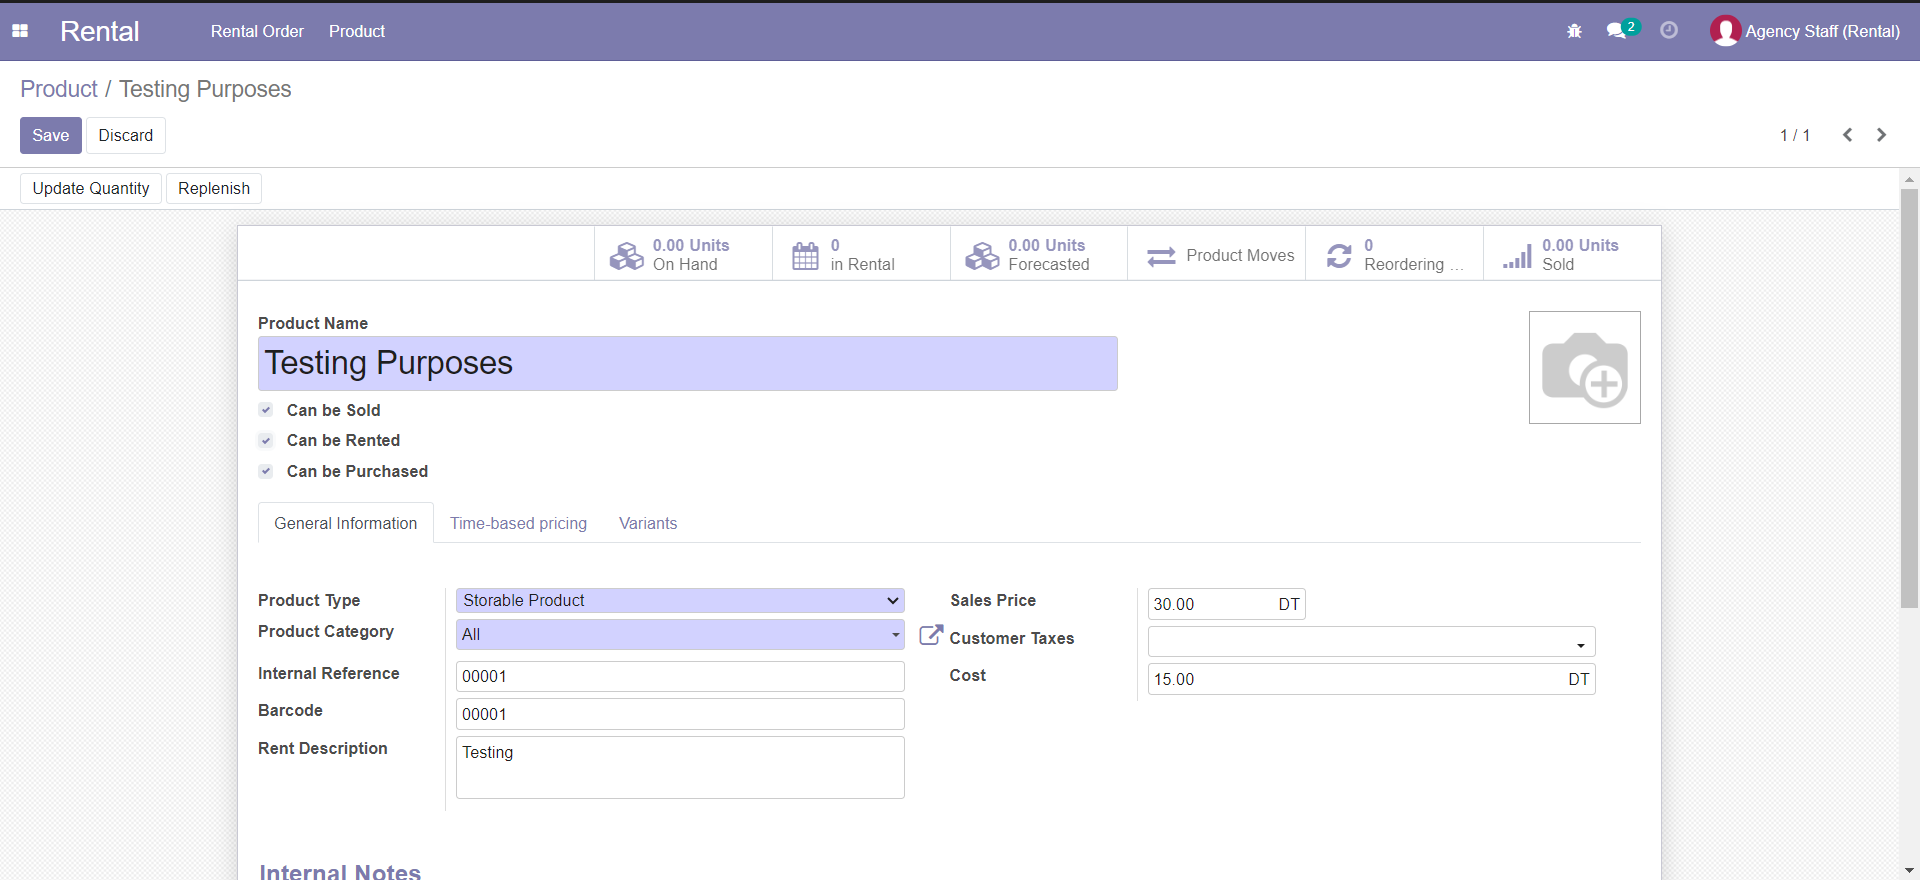
\includegraphics[width=1.2\textwidth]{sprint1/product1.png}} % replace with your image path
    \caption{General Information Notebook}
    \label{fig:general_information}
\end{figure}
\newpage

\subsection{Time-Based Pricing Notebook}
The "Time-Based Pricing" notebook is designed for rental products, allowing users to configure pricing based on different rental periods, such as hourly, daily, or weekly rates.
\begin{figure}[h]
    \centering
    \makebox[\textwidth][c]{%
        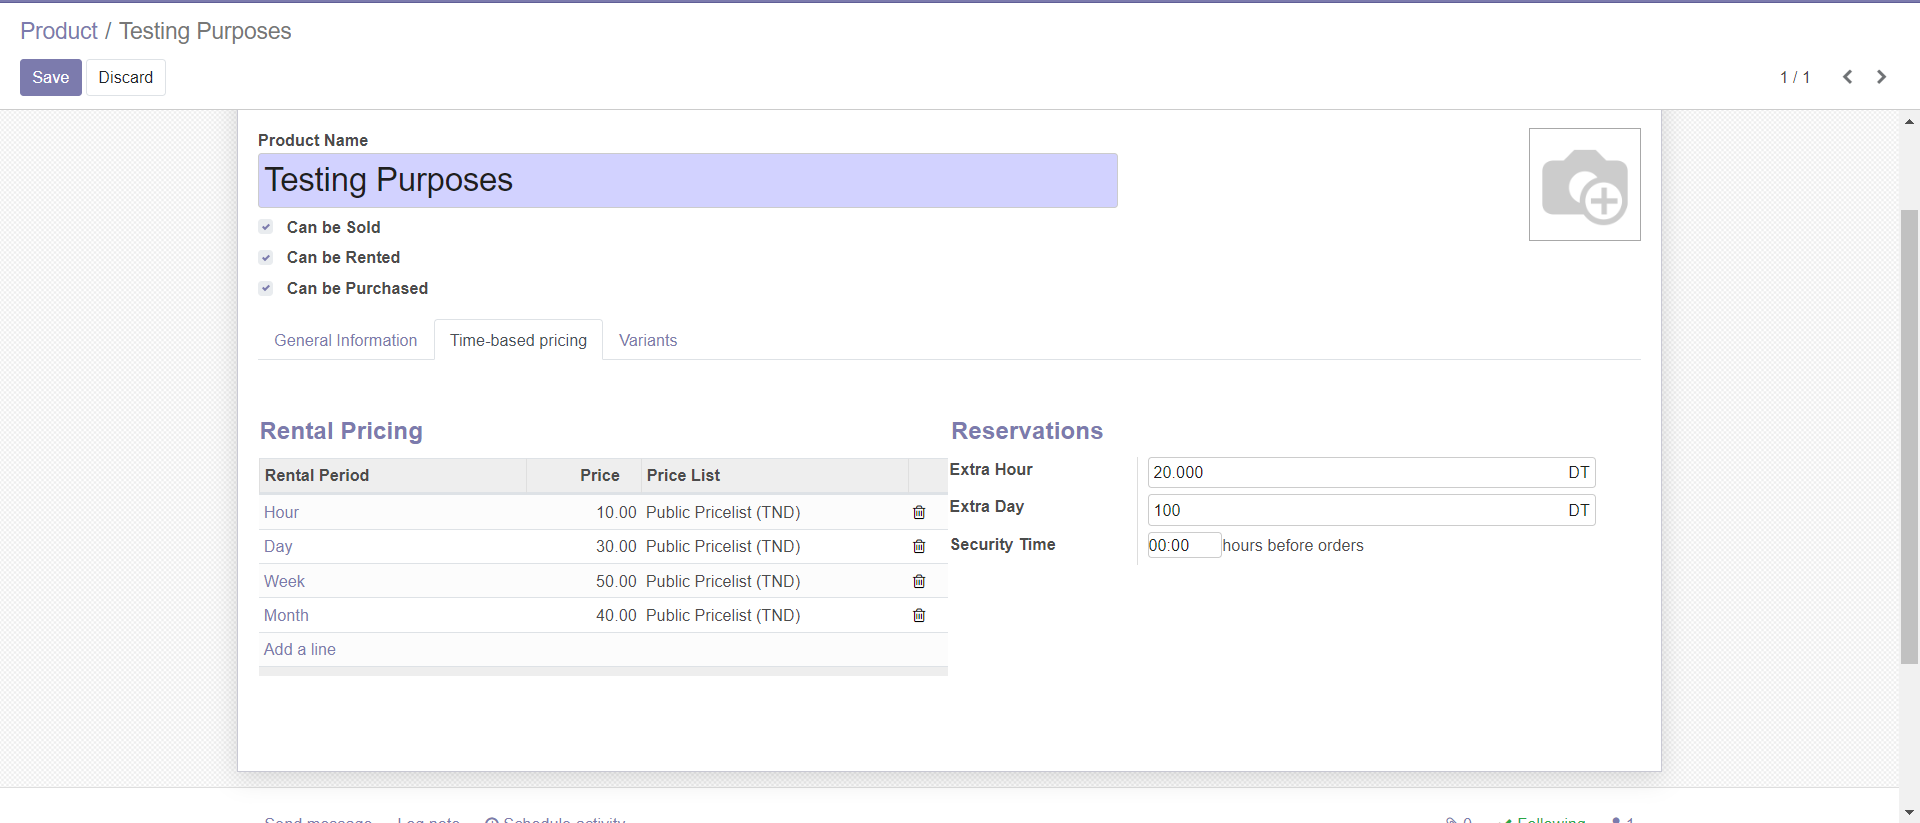
\includegraphics[width=1.2\textwidth]{sprint1/product2.png}} % replace with your image path
    \caption{Time-Based Pricing Notebook}
    \label{fig:time_based_pricing}
\end{figure}

\subsection{Variants Notebook}
The "Variants" notebook manages product variants, enabling the creation and editing of different versions of a product with various attributes like size and color, ensuring accurate representation and pricing within the product catalog.
\begin{figure}[h]
    \centering
    \makebox[\textwidth][c]{%
        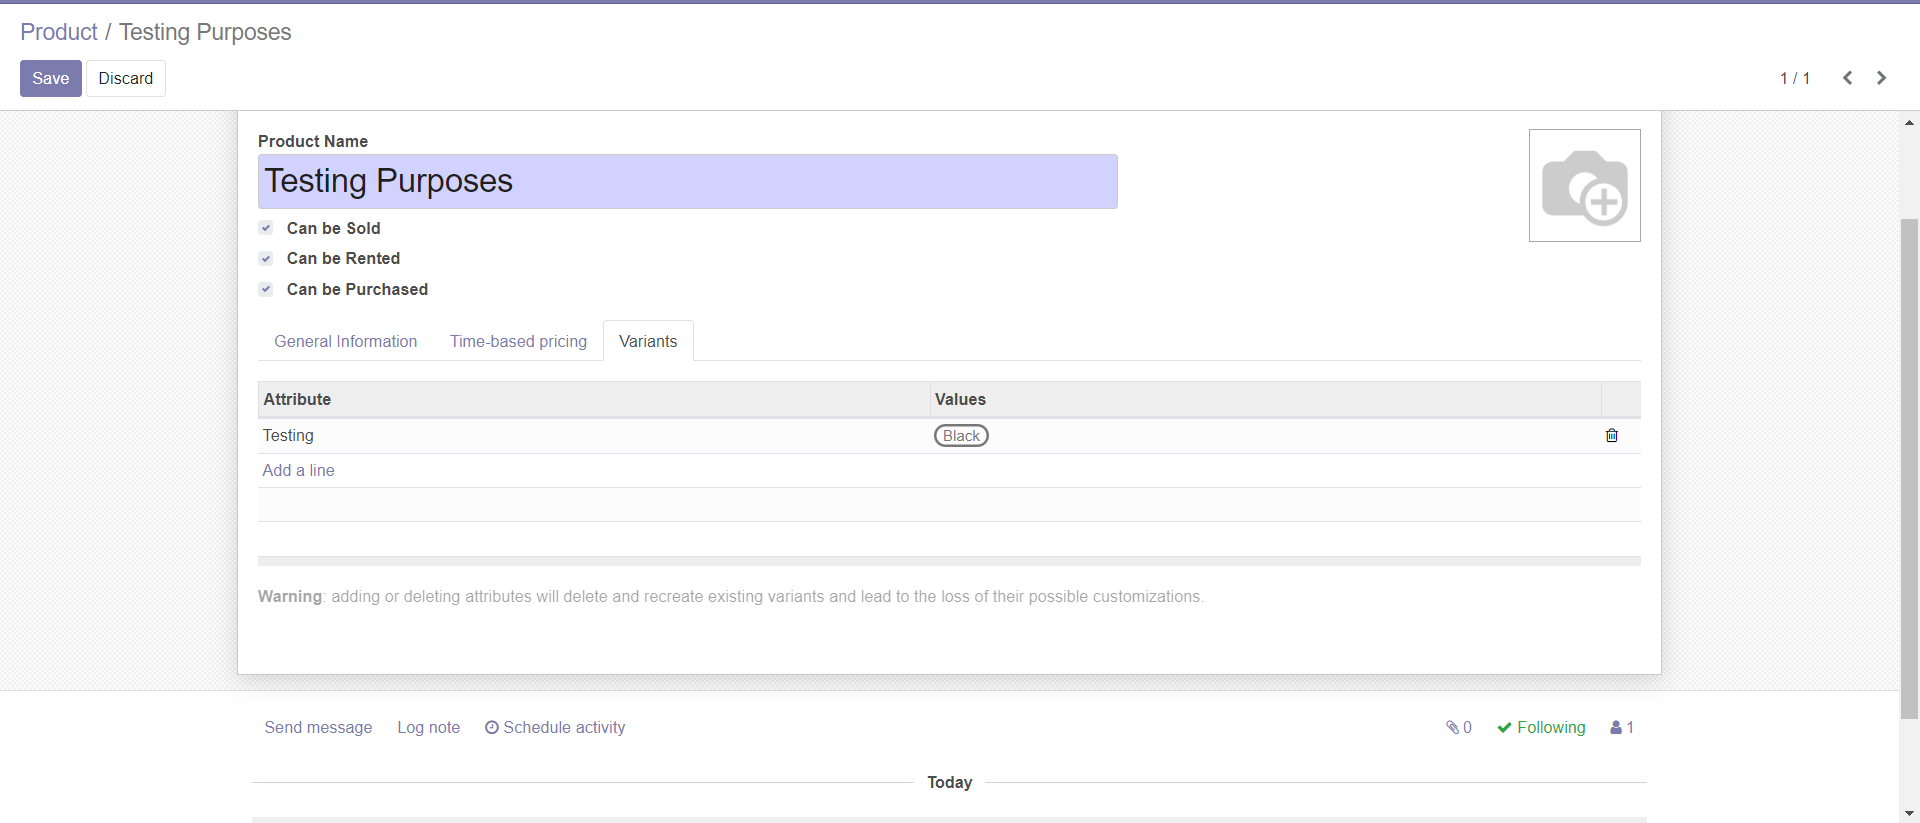
\includegraphics[width=1.2\textwidth]{sprint1/product3.png}} % replace with your image path
    \caption{Variants Notebook}
    \label{fig:variants}
\end{figure}

\subsection{Update Quantity Button}
The "Update Quantity" button allows administrators to manually adjust the stock levels of a product, ensuring inventory accuracy by reflecting real-time changes in stock quantities.
\begin{figure}[h]
    \centering
    \makebox[\textwidth][c]{%
        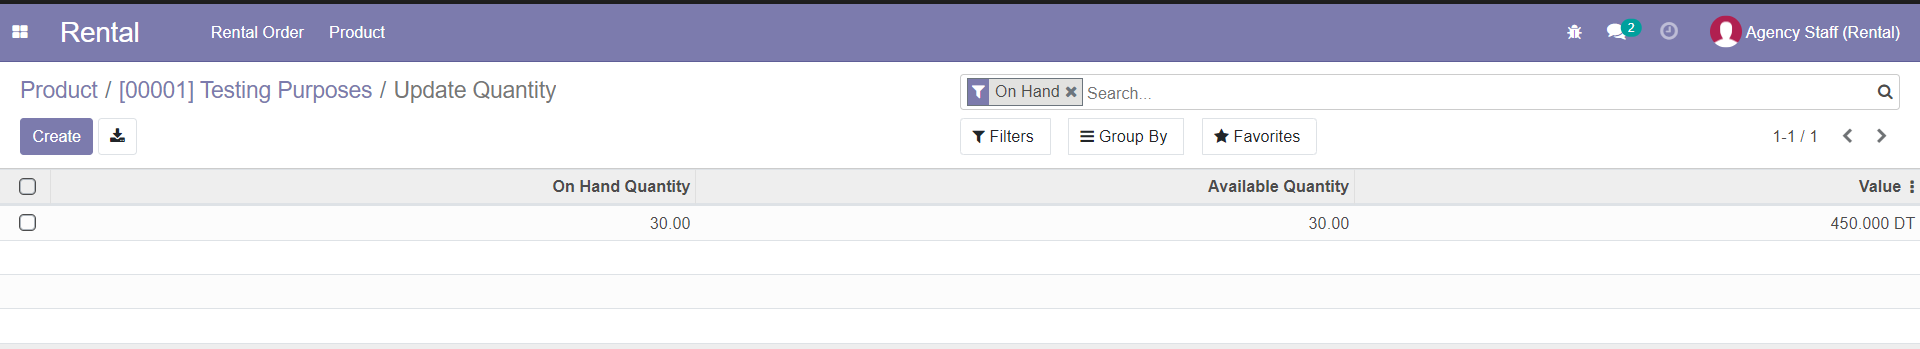
\includegraphics[width=1.2\textwidth]{sprint1/product4.png}} % replace with your image path
    \caption{Update Quantity Button}
    \label{fig:update_quantity}
\end{figure}

\subsection{Quantity on Hand Display}
After updating the quantity, the "Quantity on Hand" display reflects the new stock levels, providing an accurate overview of available inventory to help in managing stock efficiently.
\begin{figure}[h]
    \centering
    \makebox[\textwidth][c]{%
        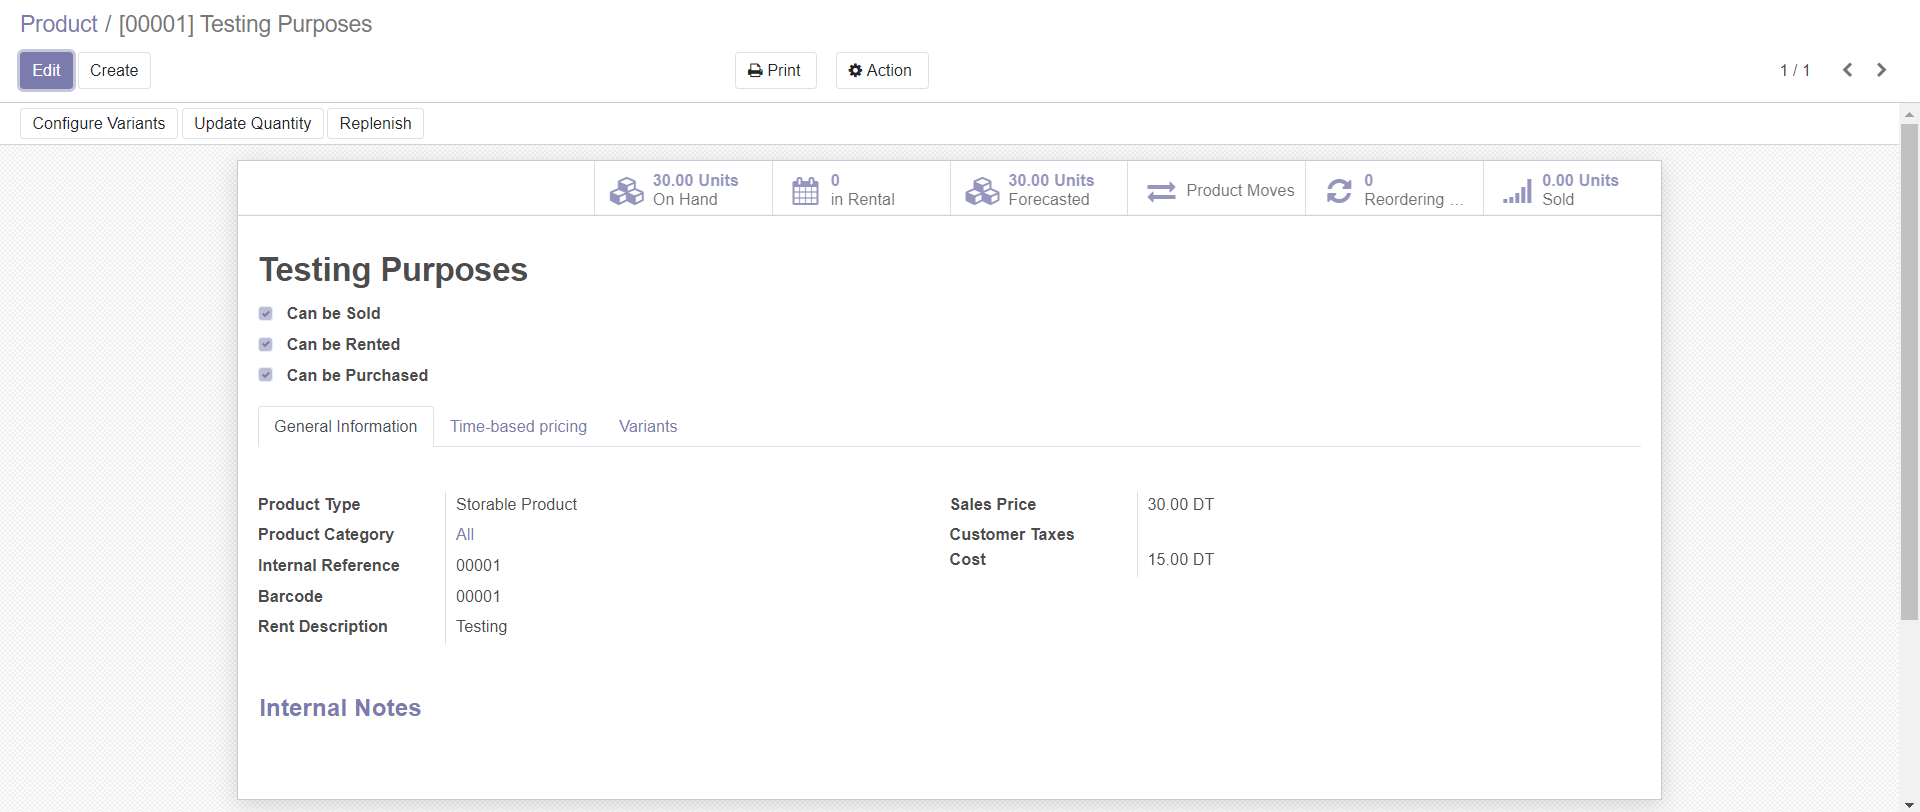
\includegraphics[width=1.2\textwidth]{sprint1/product5.png}} % replace with your image path
    \caption{Quantity on Hand Display}
    \label{fig:quantity_on_hand}
\end{figure}

\section*{Conclusion}
\addcontentsline{toc}{section}{Conclusion}
In Sprint 1, we established key functionalities in the product management module of Odoo ERP. This included "General Information," "Time-Based Pricing," and "Variants" notebooks, along with the "Update Quantity" button and "Quantity on Hand" display, enhancing product management and inventory accuracy.

In the next sprint, we will focus on the rental order process, including reservations, rental stock tracking, to further support rental operations.
\chapter{Sprint 2 - Design and implementation}

\section*{Introduction}
\addcontentsline{toc}{section}{Introduction}
In this chapter, we detail the objectives and functionalities of Sprint 2, which focuses on the Rental Order Management within the Odoo ERP system.

\section{Sprint 2 Backlog}
The Sprint 2 Backlog (Table \ref{tab:sprint2_backlog}) outlines tasks related to generating rental order reports with various view modes and filters, each task accompanied by its estimated duration, facilitating efficient sprint planning and resource allocation.

\begin{longtable}{|c|p{8cm}|c|}
    \hline
    \rowcolor{purple!20} \textbf{N°} & \textbf{Tasks} & \textbf{Duration} \\ \hline
    \endfirsthead
    \hline
    \rowcolor{purple!20} \textbf{N°} & \textbf{Tasks} & \textbf{Duration} \\ \hline
    \endhead
    1 & As an administrator, I can manage rental orders for products. & 3 Day \\ \hline
    2 & As a member, I can view my rental order history. & 1 Days \\ \hline
    3 & As an administrator, I can generate rental order reports. & 4 Day \\ \hline
    4 & As a member, I can reserve products for a specific date and time. & 6 Day \\ \hline
    5 & As an administrator, I can view and manage product reservations. & 3 Day \\ \hline
    6 & As an administrator, I can confirm or cancel reservations. & 1 Days \\ \hline
    7 & As an administrator, I can track stock levels for each product. & 6 Day \\ \hline
    8 & As an administrator, I can receive new stock shipments and update inventory. & 4 Day \\ \hline
    9 & As an administrator, I can set low stock alerts for products. & 2 Day \\ \hline
    10 & As an administrator, I can view the timeline of product rentals. & 3 Day \\ \hline
    11 & As an administrator, I can track rental durations and return dates. & 4 Day \\ \hline
    \caption{Sprint 2 Backlog for Rental Order Management, Stock Management, and Rental Timeline}
    \label{tab:sprint2_backlog}
\end{longtable}

\section{Functional Specifications}

\subsection{Use Case Diagram}
In this section, we present the functional specifications for the Rental Order Management module.
\newpage
\begin{figure}[h]
    \centering
    \makebox[\textwidth][c]{%
        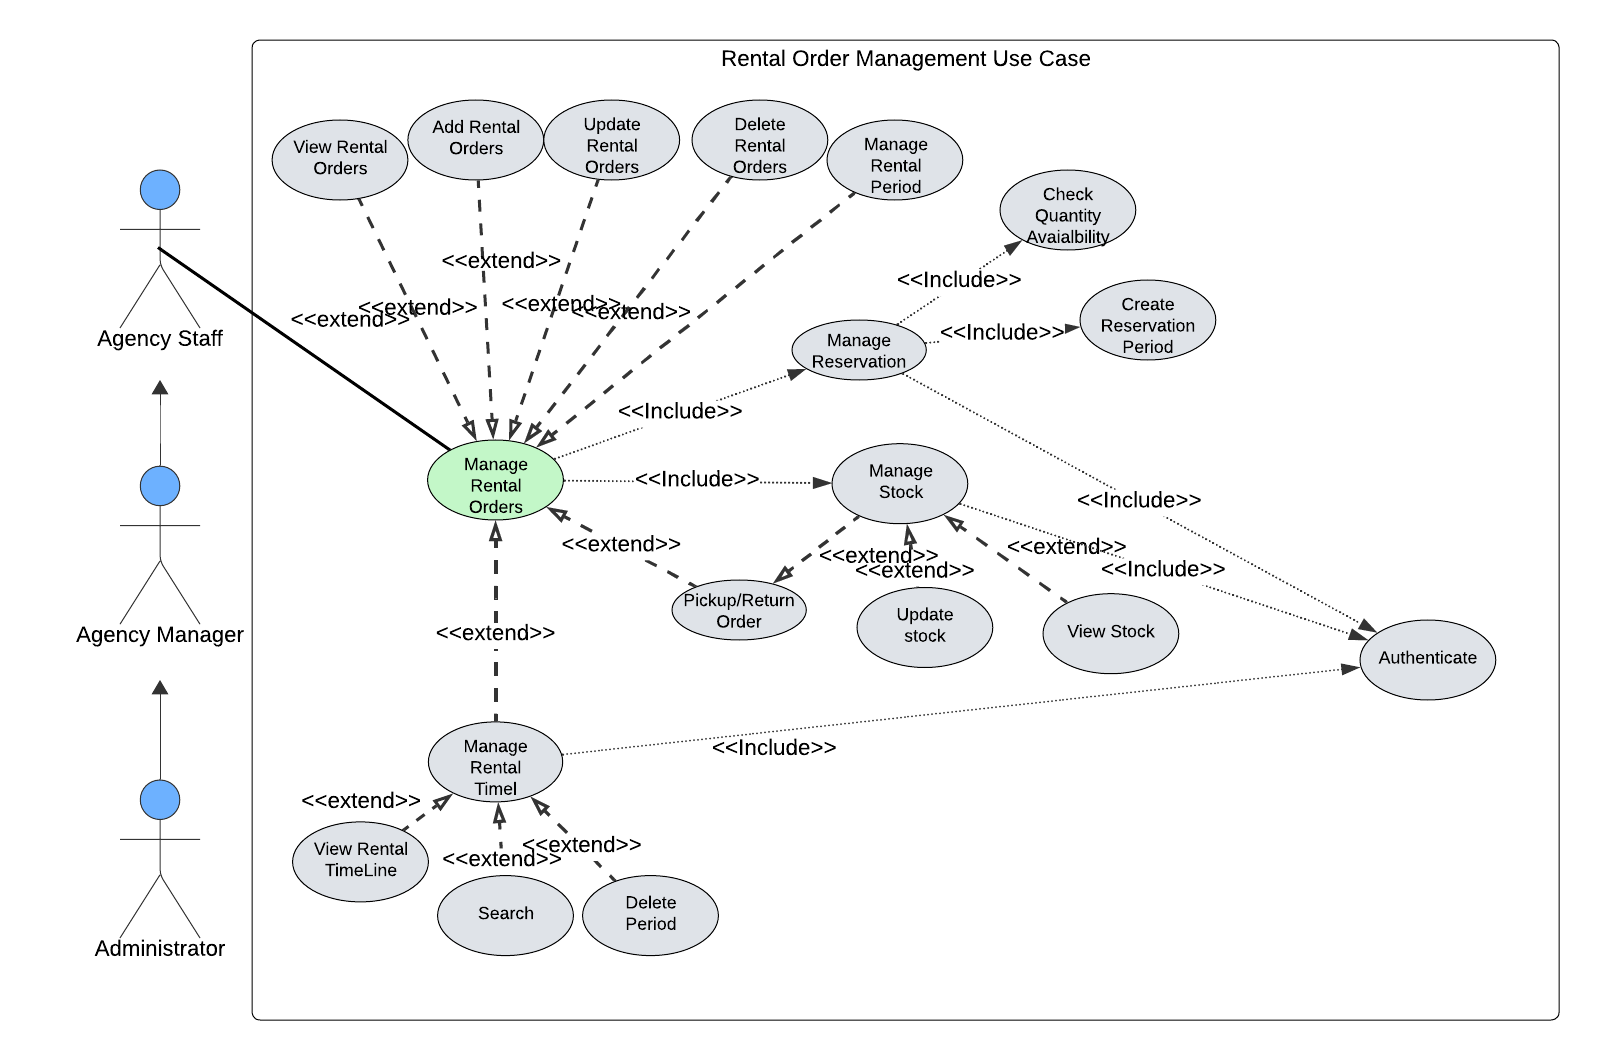
\includegraphics[width=1.2\textwidth]{sprint2/sprint2usecase.png}} % replace with your image path
    \caption{Use Case Diagram for Rental Order Management}
    \label{fig:sprint2_use_case_diagram}
\end{figure}

\subsection{Rental Order Sequence Diagram}
We present a dynamic model illustrating key scenarios of the most important use cases for Sprint 2 in the form of a sequence diagram. the process of creating a rental order:

\begin{itemize}
    \item The administrator initiates the creation of a new rental order.
    \item The system displays a rental order creation form.
    \item The administrator fills out the form with relevant details and submits it.
    \item The rental reservation model verifies and confirms the creation of the rental order.
    \item The system updates the rental stock based on the new order.
    \item The rental order state changes to reserved
    \item If the data is invalid or missing, the form remains in edit mode for correction.
    \item The administrator corrects and resubmits the data.
\end{itemize}

As depicted in Figure \ref{fig:rental_order_sequence_diagram}, the sequence diagram illustrates the "Rental Order Process" in detail.

\begin{figure}[h]
    \centering
    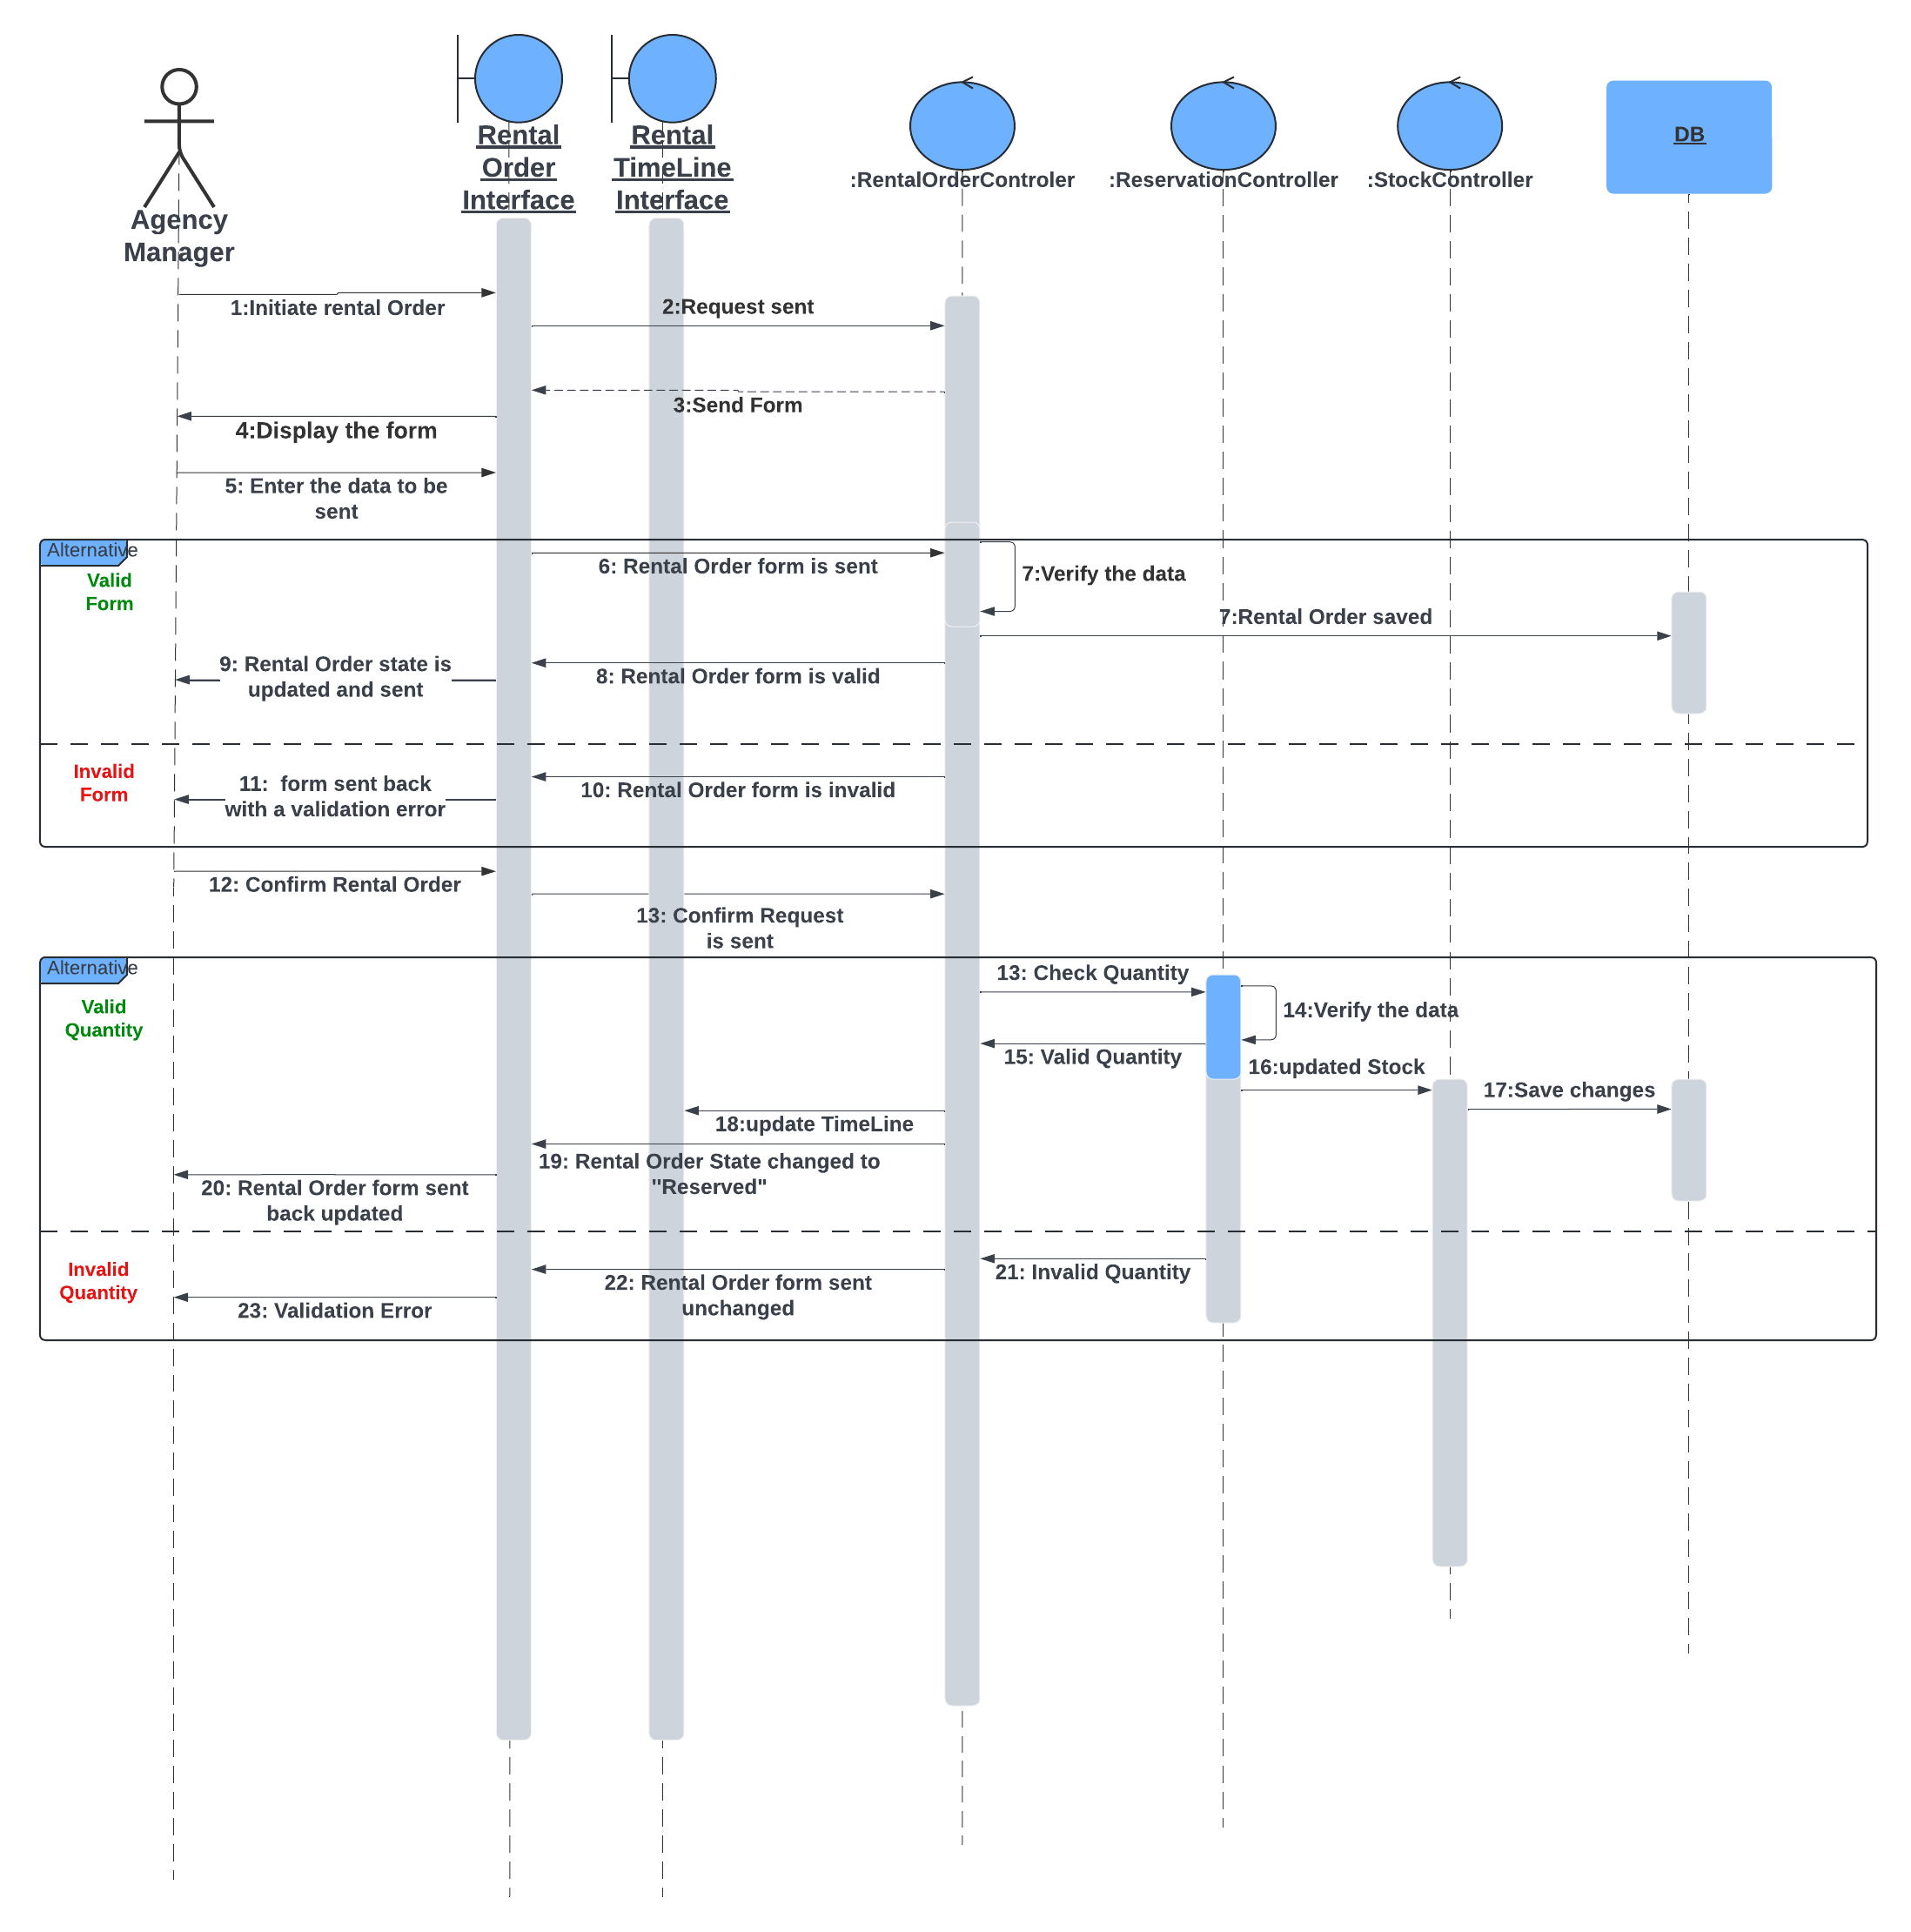
\includegraphics[width=1\textwidth]{sprint2/Sprint2Sequence1.png}
    \caption{Sequence Diagram for "Rental Order Process"}
    \label{fig:rental_order_sequence_diagram}
\end{figure} 
\newpage
\subsection{Pickup and Retur Order Sequence Diagram}

\begin{itemize}
    \item \textbf{Picking Up Rental Items:}
    \begin{itemize}
        \item The administrator initiates the pickup process for the rental order.
        \item The system displays the Pickup Order Wizard.
        \item The administrator specifies the quantities to be collected for each rental item.
        \item The system updates the rental stock to reflect the picked up quantities.
        \item The rental order state changes to rented if all items are picked up.
        \item If quantities are insufficient or other errors occur, the process handles alternatives.
    \end{itemize}
    \item \textbf{Returning Rental Items:}
    \begin{itemize}
        \item The administrator initiates the return process for the rental order.
        \item The system displays the Return Order Wizard.
        \item The administrator specifies quantities to be returned for each rental item.
        \item The system updates the rental stock to reflect the returned quantities and return dates.
        \item The rental order state changes to done if all items are returned.
        \item If quantities are insufficient or other errors occur, the process handles alternatives.
    \end{itemize}
\end{itemize}
\newpage
As shown in Figure \ref{fig:pickup_return_ordersequence_diagram}, the sequence diagram depicts the process of "Pickup/Return" orders.

\begin{figure}[h]
    \centering
    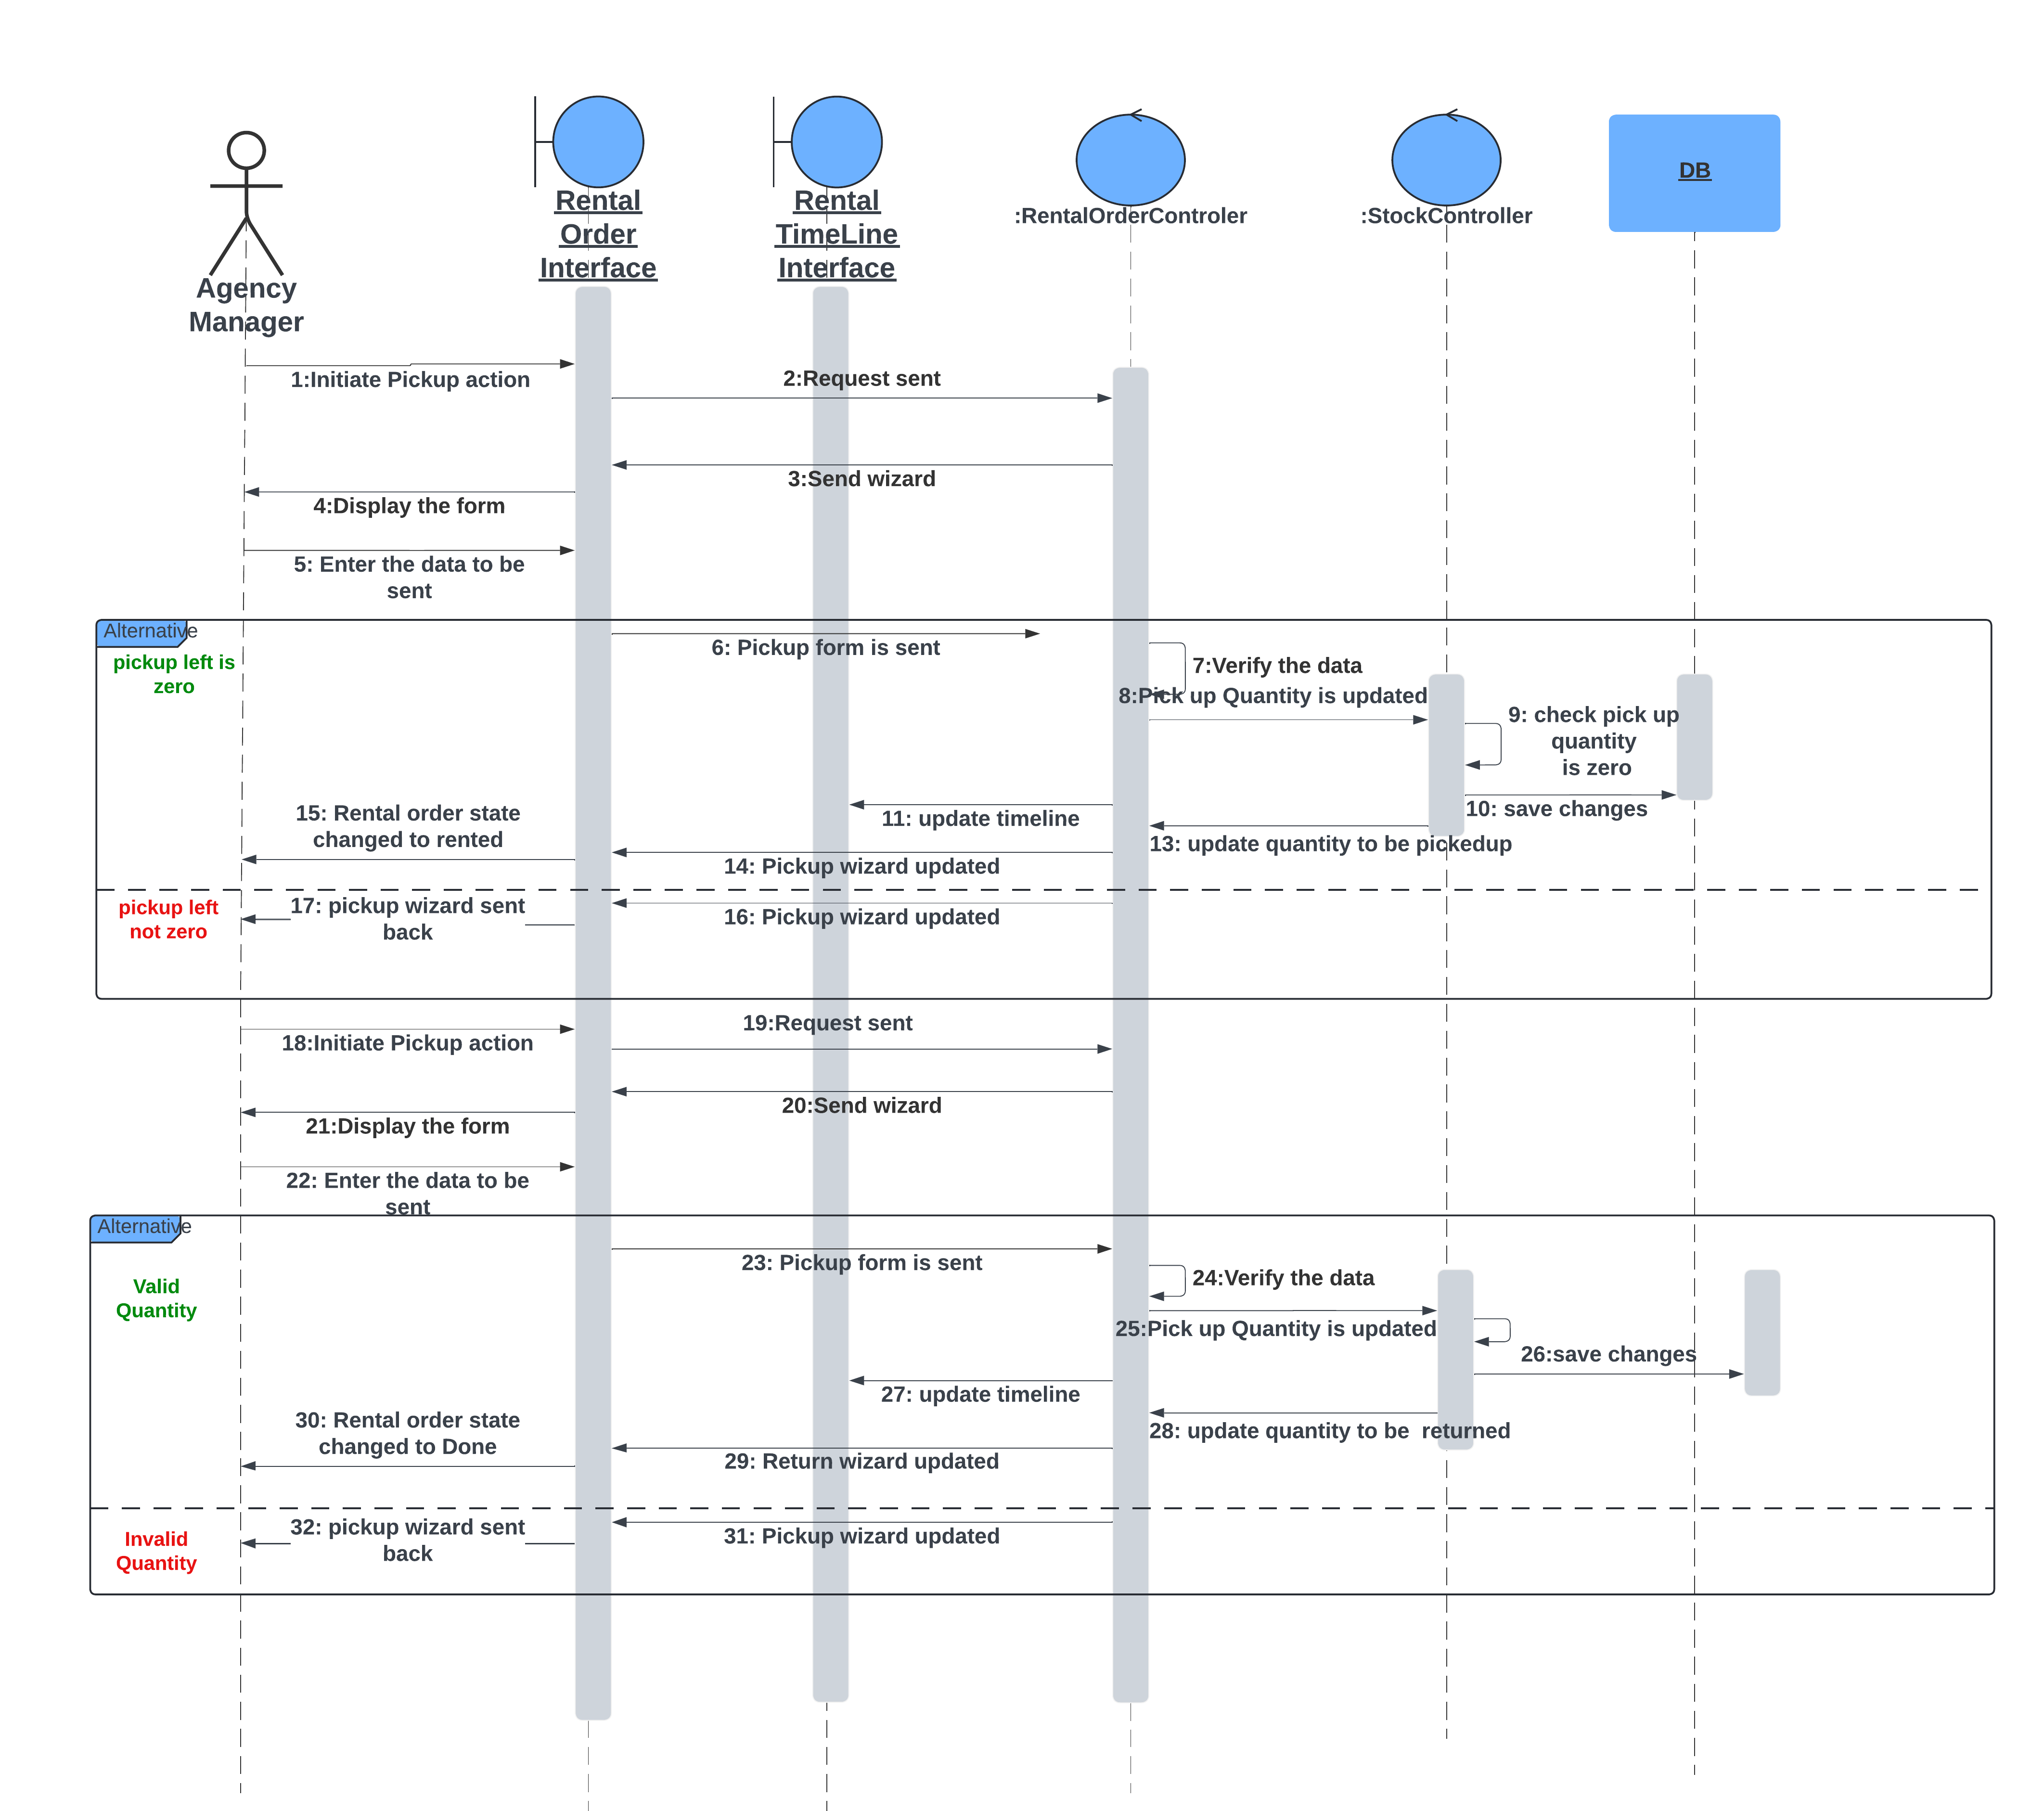
\includegraphics[width=1\textwidth]{sprint2/Sprint2Sequence2.png}
    \caption{Sequence Diagram for "Pickup/Return" Order}
    \label{fig:pickup_return_ordersequence_diagram}
\end{figure}

\section{Sprint Realization}
\subsection{Rental Order Form}
The screenshot in Figure \ref{fig:rental_order_form} displays the initial rental order form where the administrator fills out details such as customer information, rental duration, and selected products.
\newpage
% \begin{figure}[h]
%     \centering
%     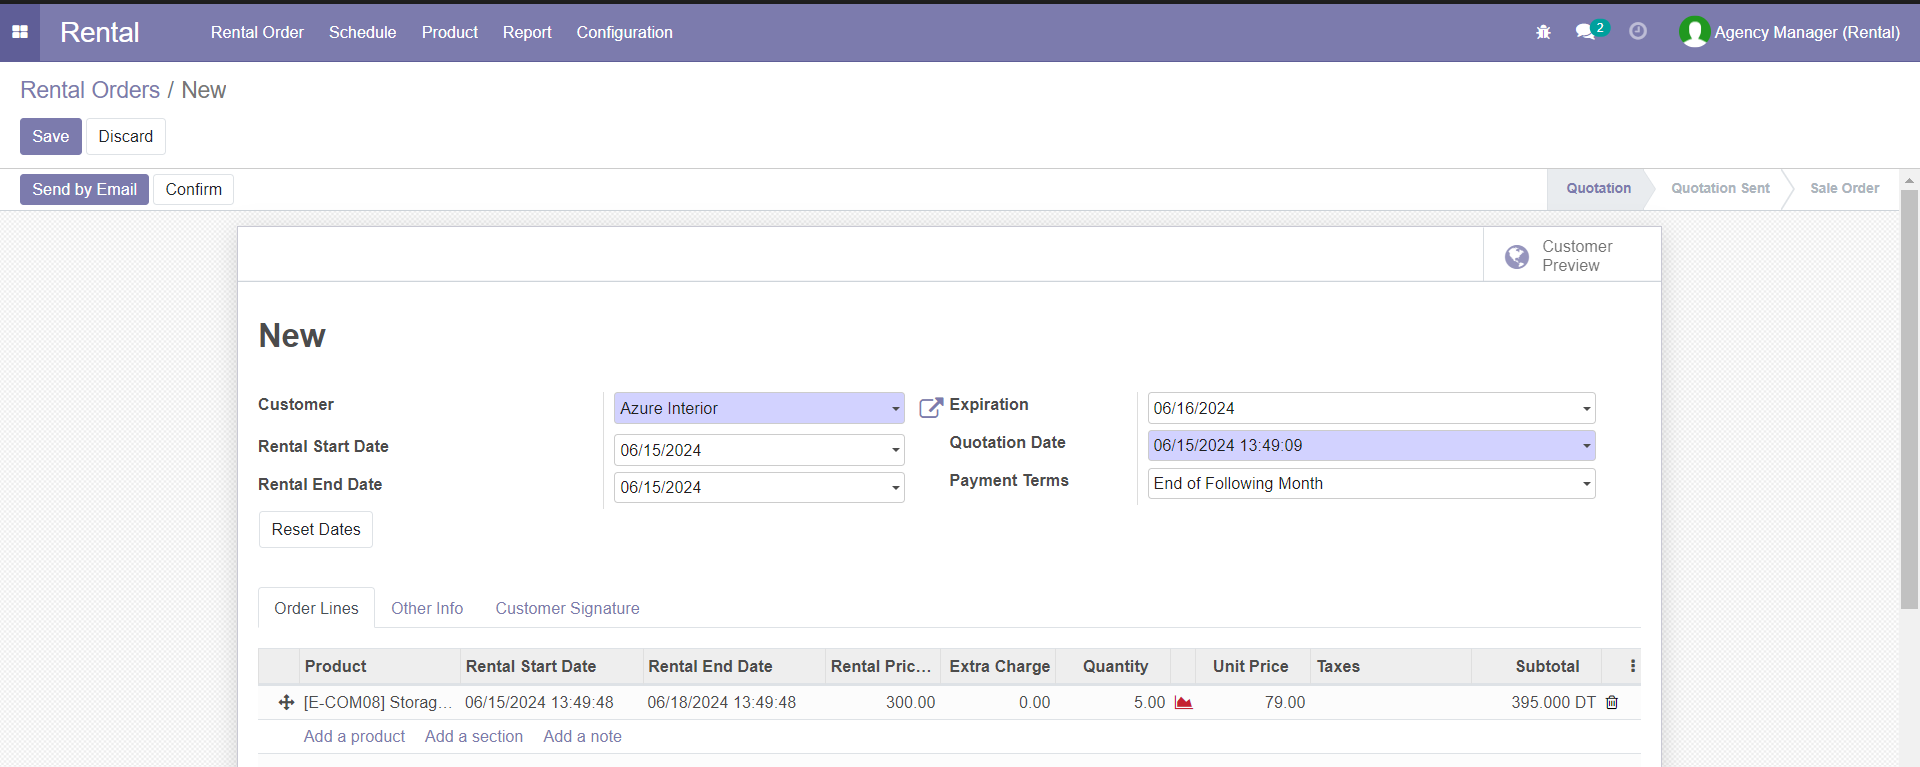
\includegraphics[width=1\textwidth]{sprint2/rentalorder1.png}
%     \caption{Screenshot of Rental Order Form}
%     \label{fig:rental_order_form}
% \end{figure}
\begin{figure}[h]
    \centering
    \makebox[\textwidth][c]{%
        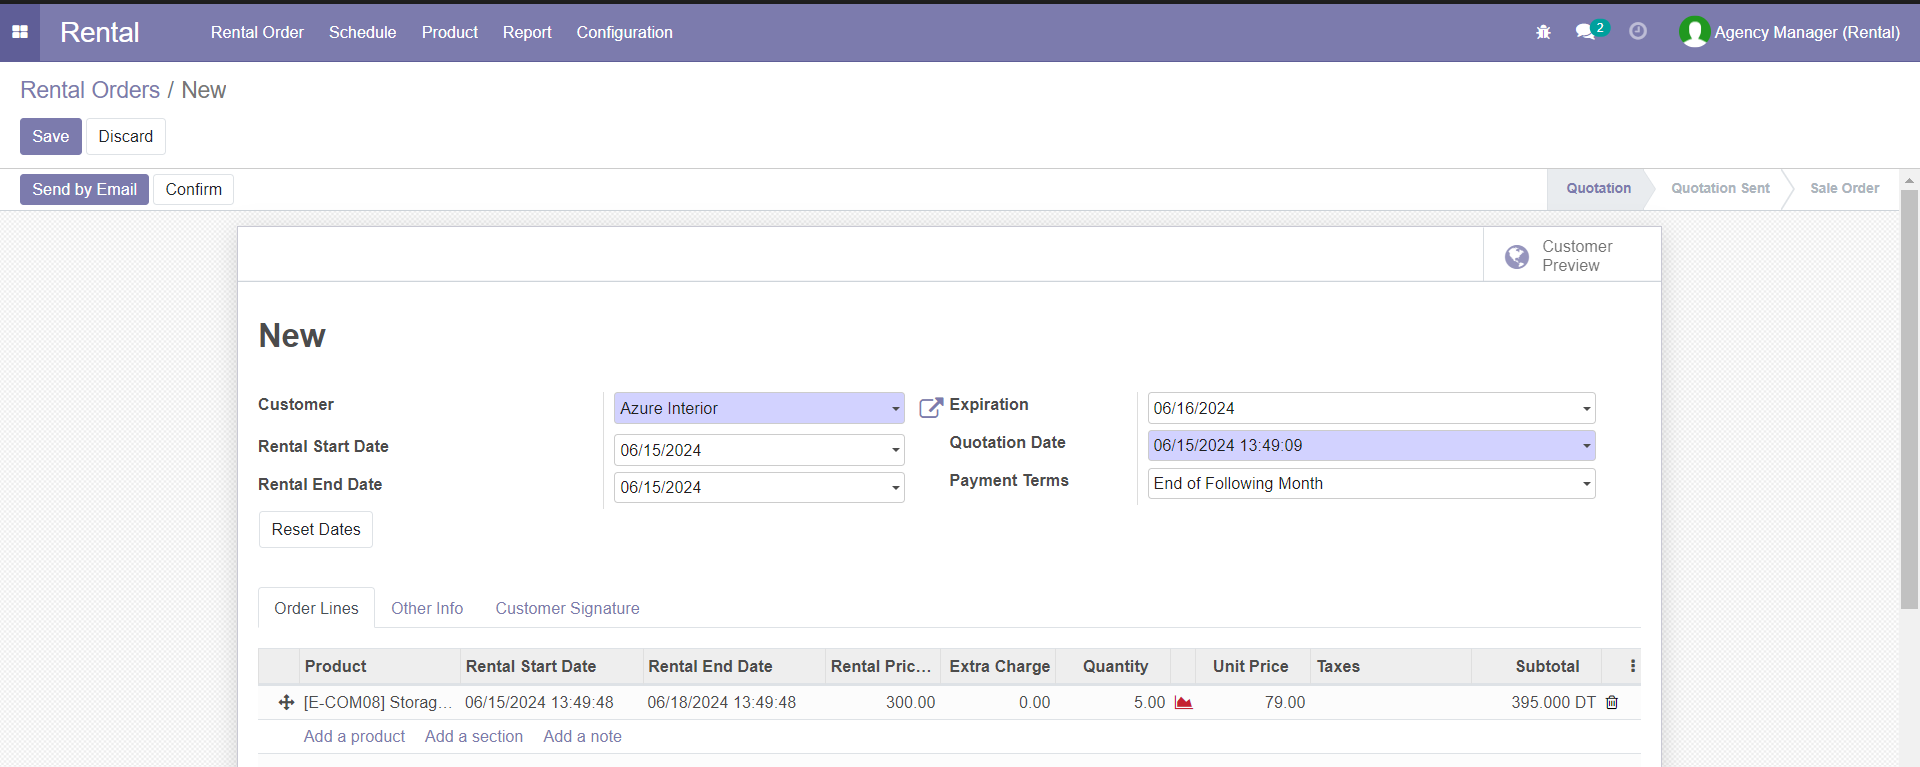
\includegraphics[width=1.2\textwidth]{sprint2/rentalorder1.png}} % replace with your image path
    \caption{Screenshot of Rental Order Form}
    \label{fig:rental_order_form}
\end{figure}

\subsection{Confirmed Rental Order}
Figure \ref{fig:confirmed_rental_order} illustrates the confirmation screen of the rental order after submission. It indicates successful validation and reservation of rental items.

% \begin{figure}[h]
%     \centering
%     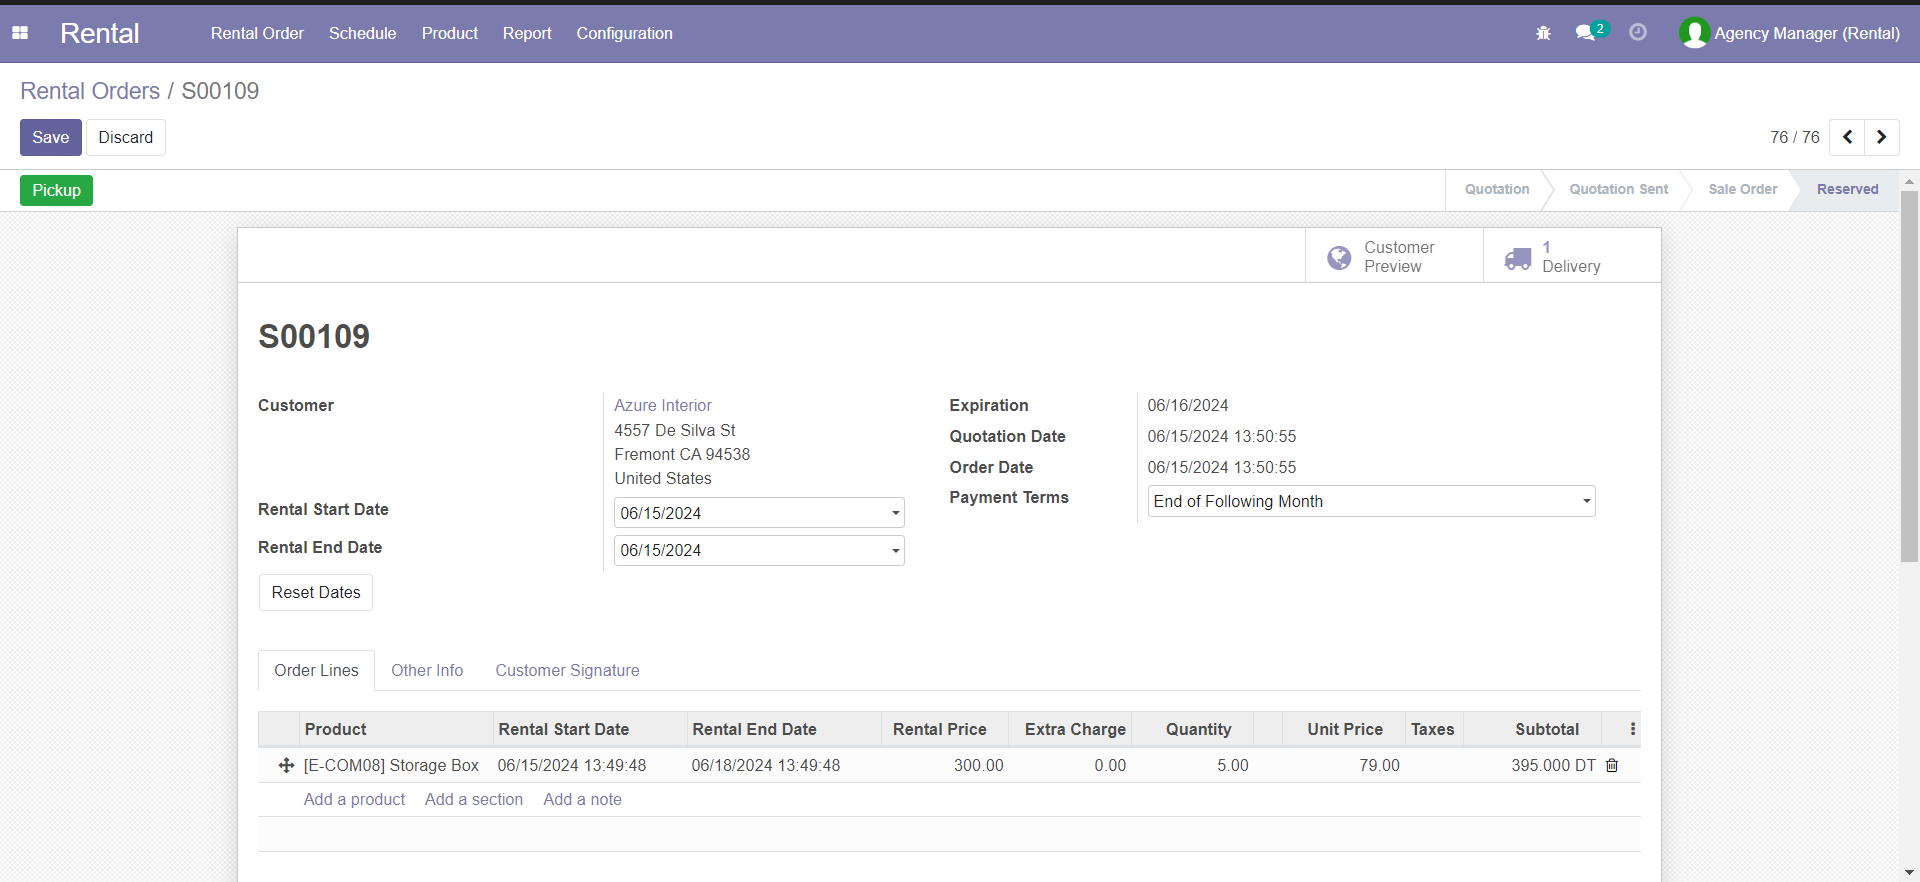
\includegraphics[width=1\textwidth]{sprint2/rentalorder2.png}
%     \caption{Screenshot of Confirmed Rental Order}
%     \label{fig:confirmed_rental_order}
% \end{figure}
\begin{figure}[h]
    \centering
    \makebox[\textwidth][c]{%
        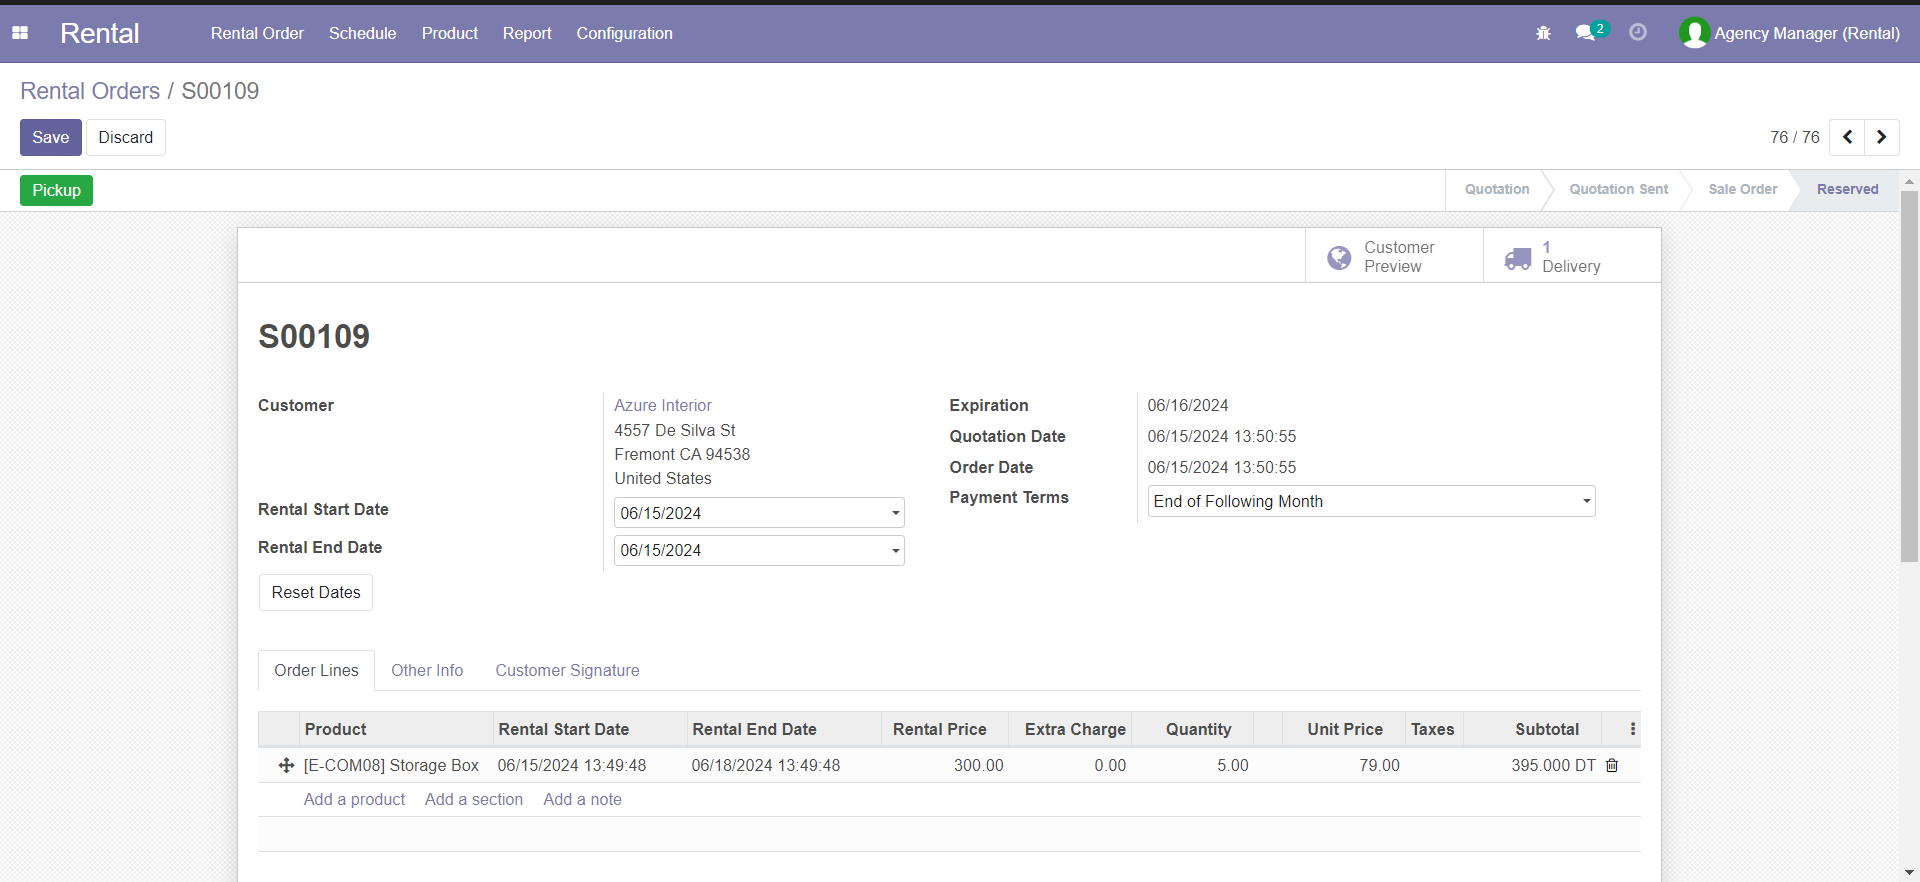
\includegraphics[width=1.2\textwidth]{sprint2/rentalorder2.png}} % replace with your image path
    \caption{Screenshot of Confirmed Rental Order}
    \label{fig:confirmed_rental_order}
\end{figure}

\subsection{Pickup Wizard}
Figure \ref{fig:pickup_state} shows the Pickup Wizard where the administrator manages quantities for pickup, updating the rental stock and changing the rental order state to rented (green).

\begin{figure}[h]
    \centering
    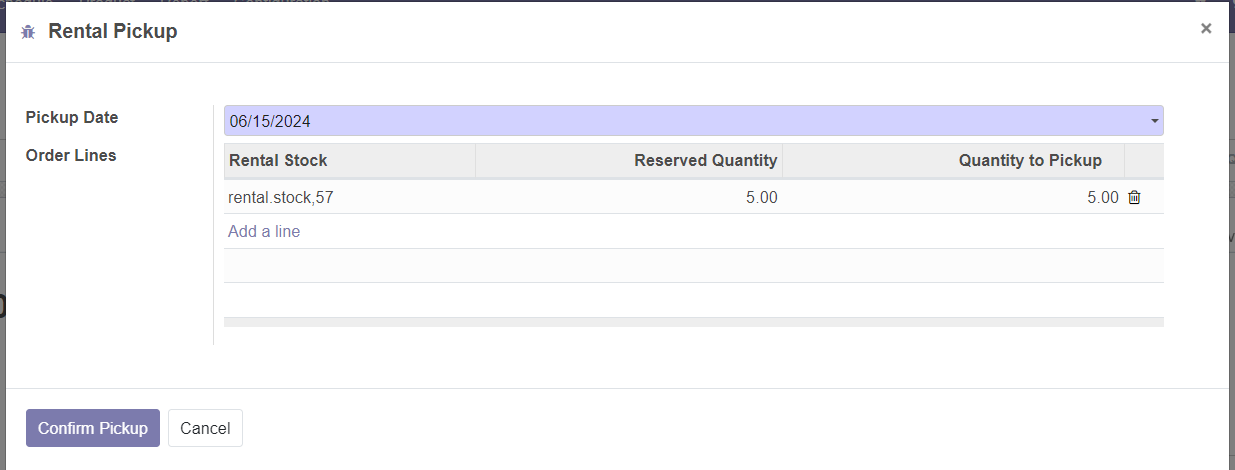
\includegraphics[width=1\textwidth]{sprint2/rentalorderpickup3.png}
    \caption{Screenshot of Pickup State}
    \label{fig:pickup_state}
\end{figure}

\subsection{Return Wizard}
Figure \ref{fig:return_state} shows the Return Wizard where the administrator manages returns, calculates any extra charges for late returns, updates the stock, and changes the rental order state to done (grey).

\begin{figure}[h]
    \centering
    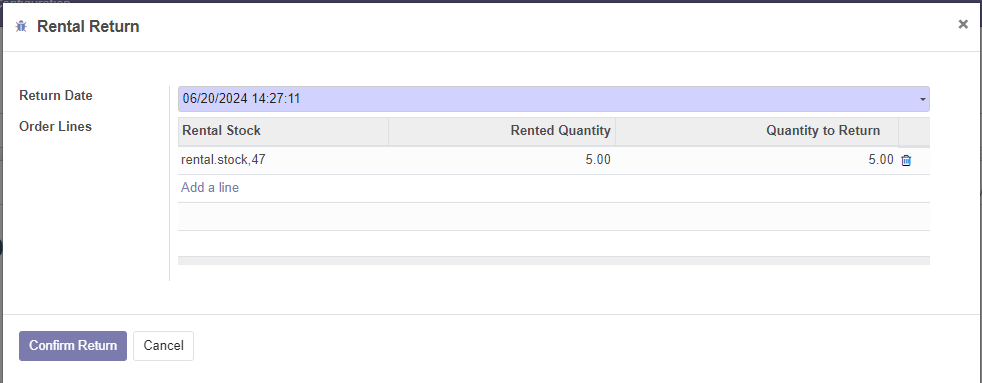
\includegraphics[width=1\textwidth]{sprint2/rentalorderreturn4.png}
    \caption{Screenshot of Return State}
    \label{fig:return_state}
\end{figure}

\subsection{Rental Stock Movement}
Figure \ref{fig:rental_stock_view} visualizes the movements of rental stock items, Each item is associated with its order ID for tracking. The stock view shows quantity updates as rental orders change.
\begin{figure}[h]
    \centering
    \makebox[\textwidth][c]{%
        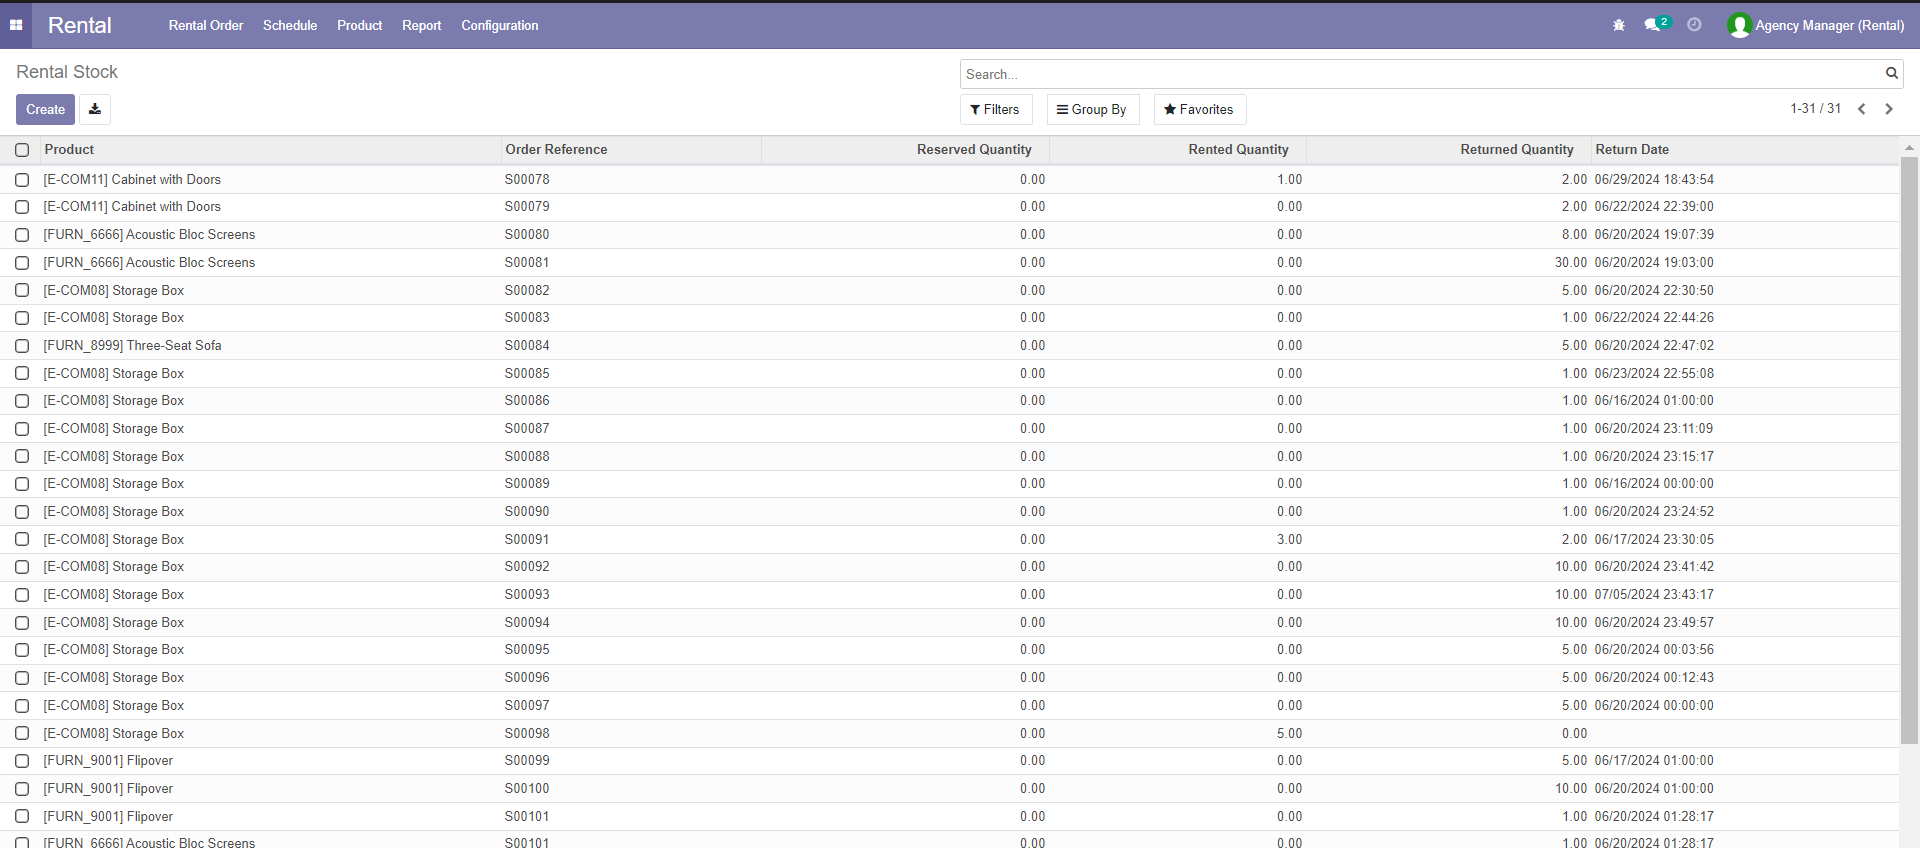
\includegraphics[width=1.2\textwidth]{sprint2/rentalorderstock7.png}} % replace with your image path
    \caption{Rental Stock View}
    \label{fig:rental_stock_view}
\end{figure}

\subsection{Rental Schedule Timeline}
Figure \ref{fig:rental_schedule_timeline} illustrates the rental schedule timeline, showing how information is grouped by product. It highlights the progress of each order through different states—reserved (blue), rented (green), and done (grey)—and includes the associated order ID for reference. The timeline updates reflect changes in rental orders.

% \begin{figure}[h]
%     \centering
%     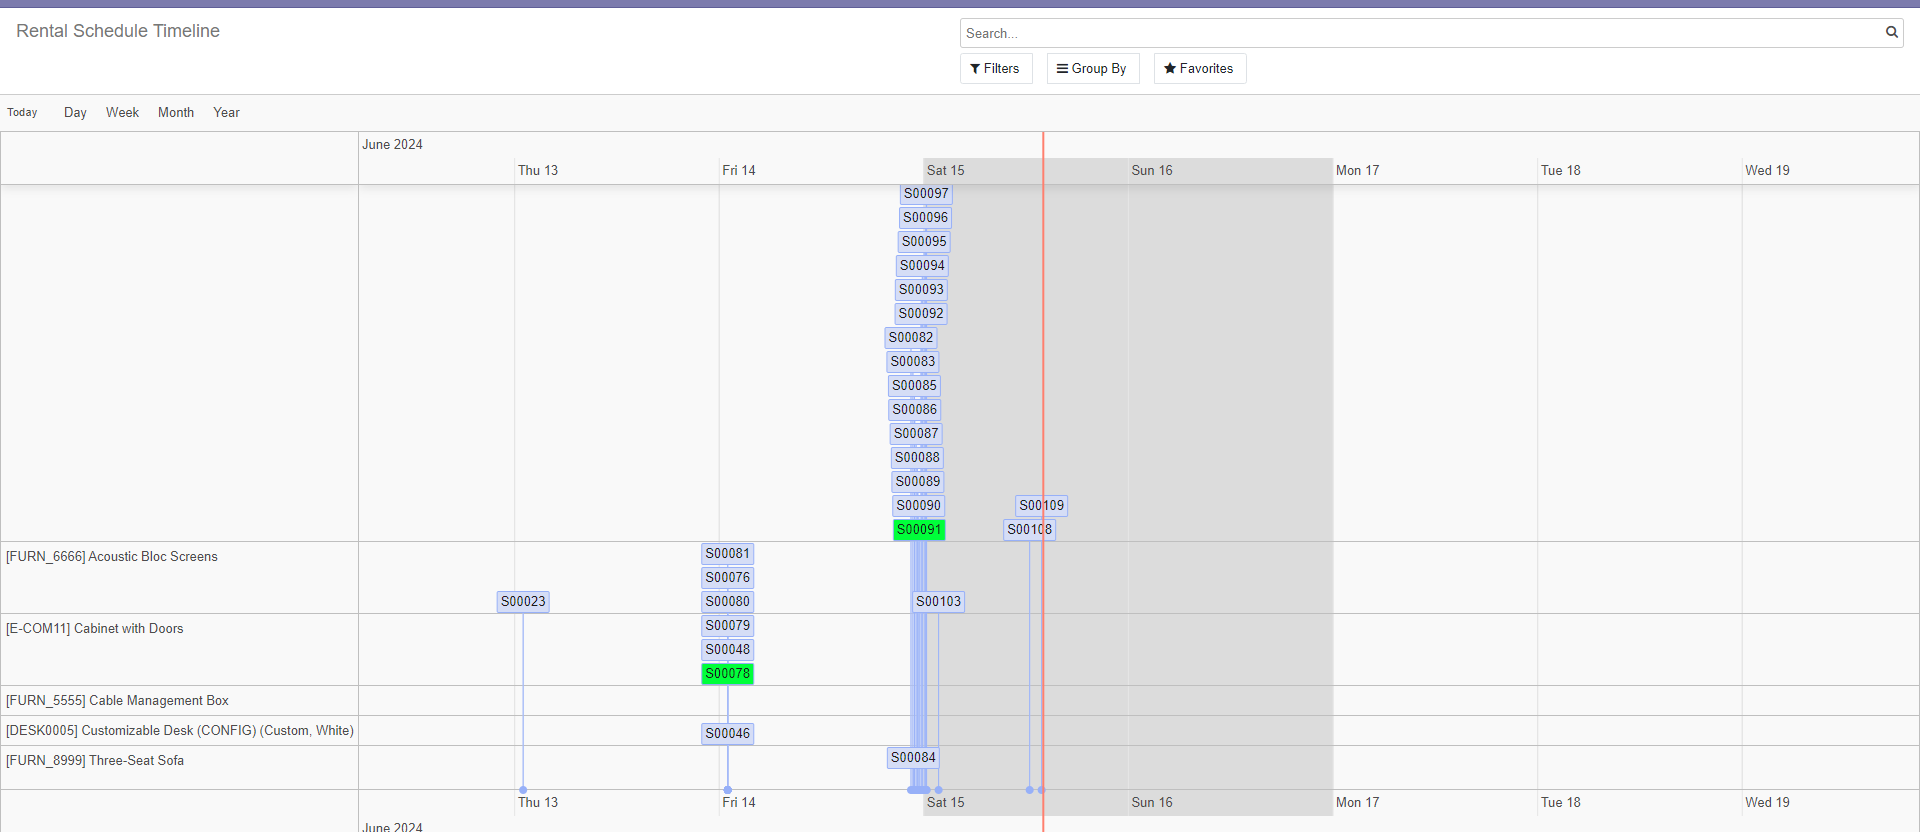
\includegraphics[width=1\textwidth]{sprint2/rentalorderschedule6.png}
%     \caption{Screenshot of Timeline}
%     \label{fig:rental_schedule_timeline}
% \end{figure}
\begin{figure}[h]
    \centering
    \makebox[\textwidth][c]{%
        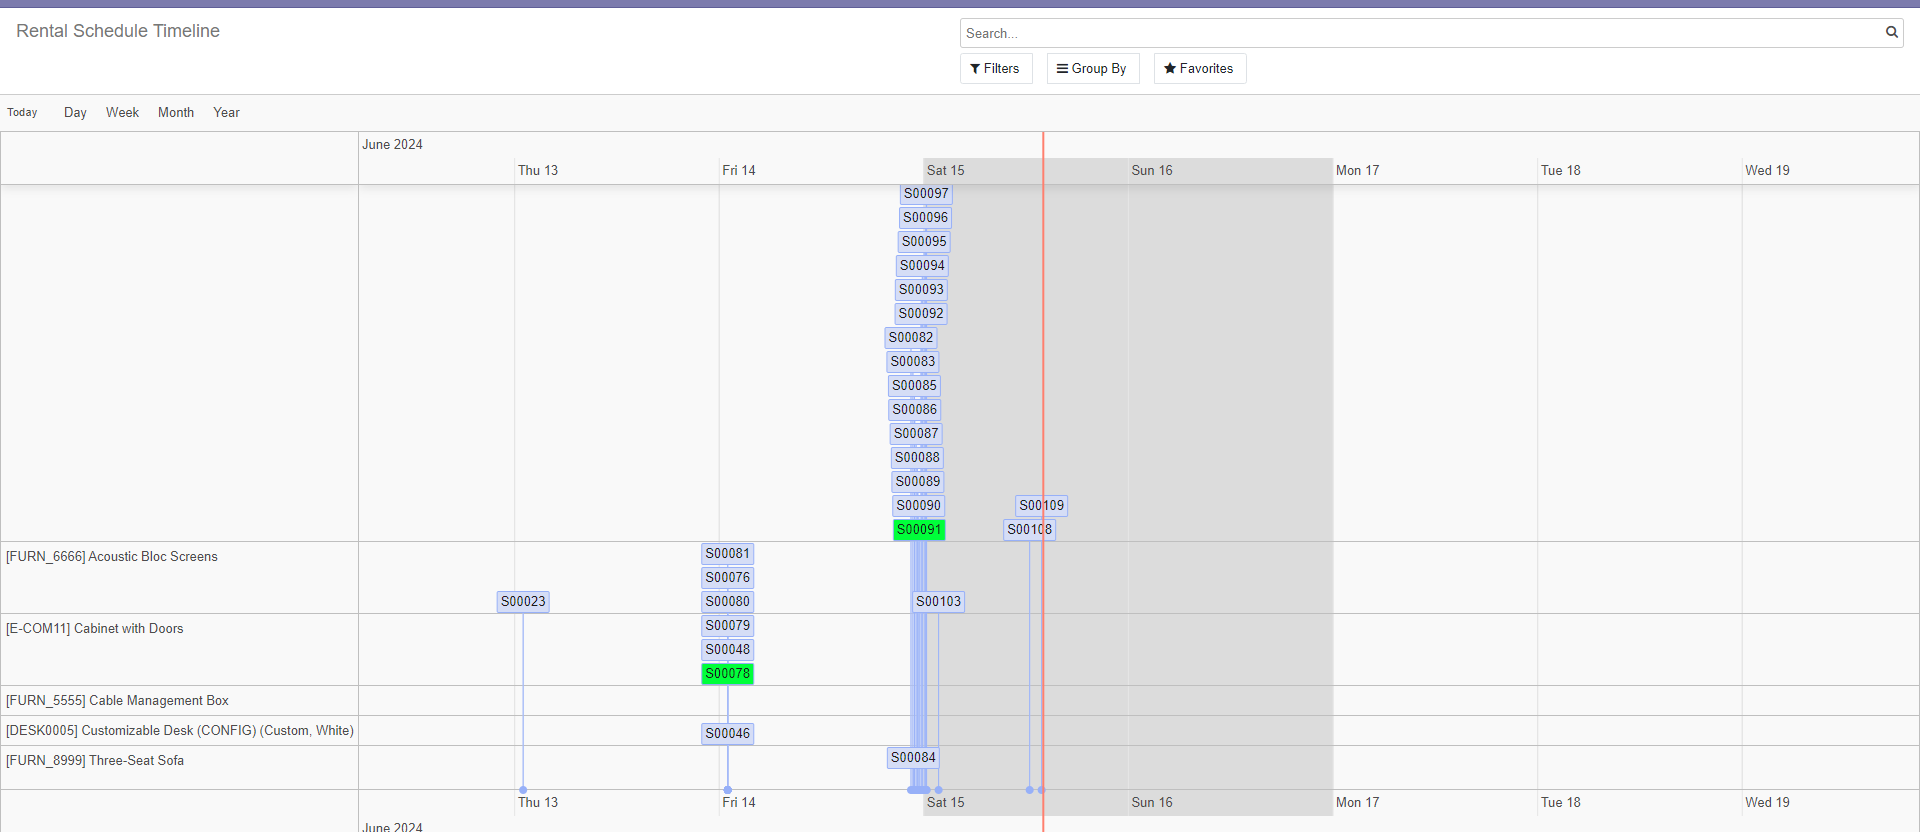
\includegraphics[width=1.1\textwidth]{sprint2/rentalorderschedule6.png}} % replace with your image path
    \caption{Screenshot of Timeline}
    \label{fig:rental_schedule_timeline}
\end{figure}
\newpage
\section*{Conclusion}
\addcontentsline{toc}{section}{Conclusion}

In Sprint 2, we established key functionalities in the rental order process module of Odoo ERP. This included the "Order Details," "Inventory Management," and "Rental Pricing" notebooks, along with the "Update Order Status" button and "Order Status" display, enhancing the rental order management process. In the next sprint, we will focus on integrating the rental order process with billing and invoicing to streamline financial operations.

\chapter{Sprint 3 - Design and implementation}

\section*{Introduction}
\addcontentsline{toc}{section}{Introduction}
In Sprint 3, administrators focused on improving rental order reporting by adding dynamic filters. 
\section{Sprint 3 Backlog}
Table \ref{tab:sprint3_backlog} lists the planned tasks for this sprint.

\begin{longtable}{|c|p{8cm}|c|}
    \hline
    \rowcolor{purple!20} \textbf{N°} & \textbf{Tasks} & \textbf{Duration} \\ \hline
    \endfirsthead
    \hline
    \rowcolor{purple!20} \textbf{N°} & \textbf{Tasks} & \textbf{Duration} \\ \hline
    \endhead
    1 & As an administrator, I can generate rental order reports. & 3 Day \\ \hline
    2 & As an administrator, I can view rental reports in different chart formats (bar, pie, line, pivot). & 3 Day \\ \hline
    3 & As an administrator, I can filter rental reports by measure (order date, customer, product). & 2 Days \\ \hline
    4 & As an administrator, I can adjust report view modes and filters dynamically. & 2 Days \\ \hline
    \caption{Sprint 3 Backlog for Rental Order Reporting}
    \label{tab:sprint3_backlog}
\end{longtable}

\section{Functional Specifications}

\subsection{Use Case Diagram}
This section presents the functional specifications for the Rental Order Reporting module. Figure \ref{fig:sprint3_use_case_diagram} depicts the use case diagram that outlines the interactions and functionalities within this module.

\begin{figure}[h]
    \centering
    \makebox[\textwidth][c]{%
        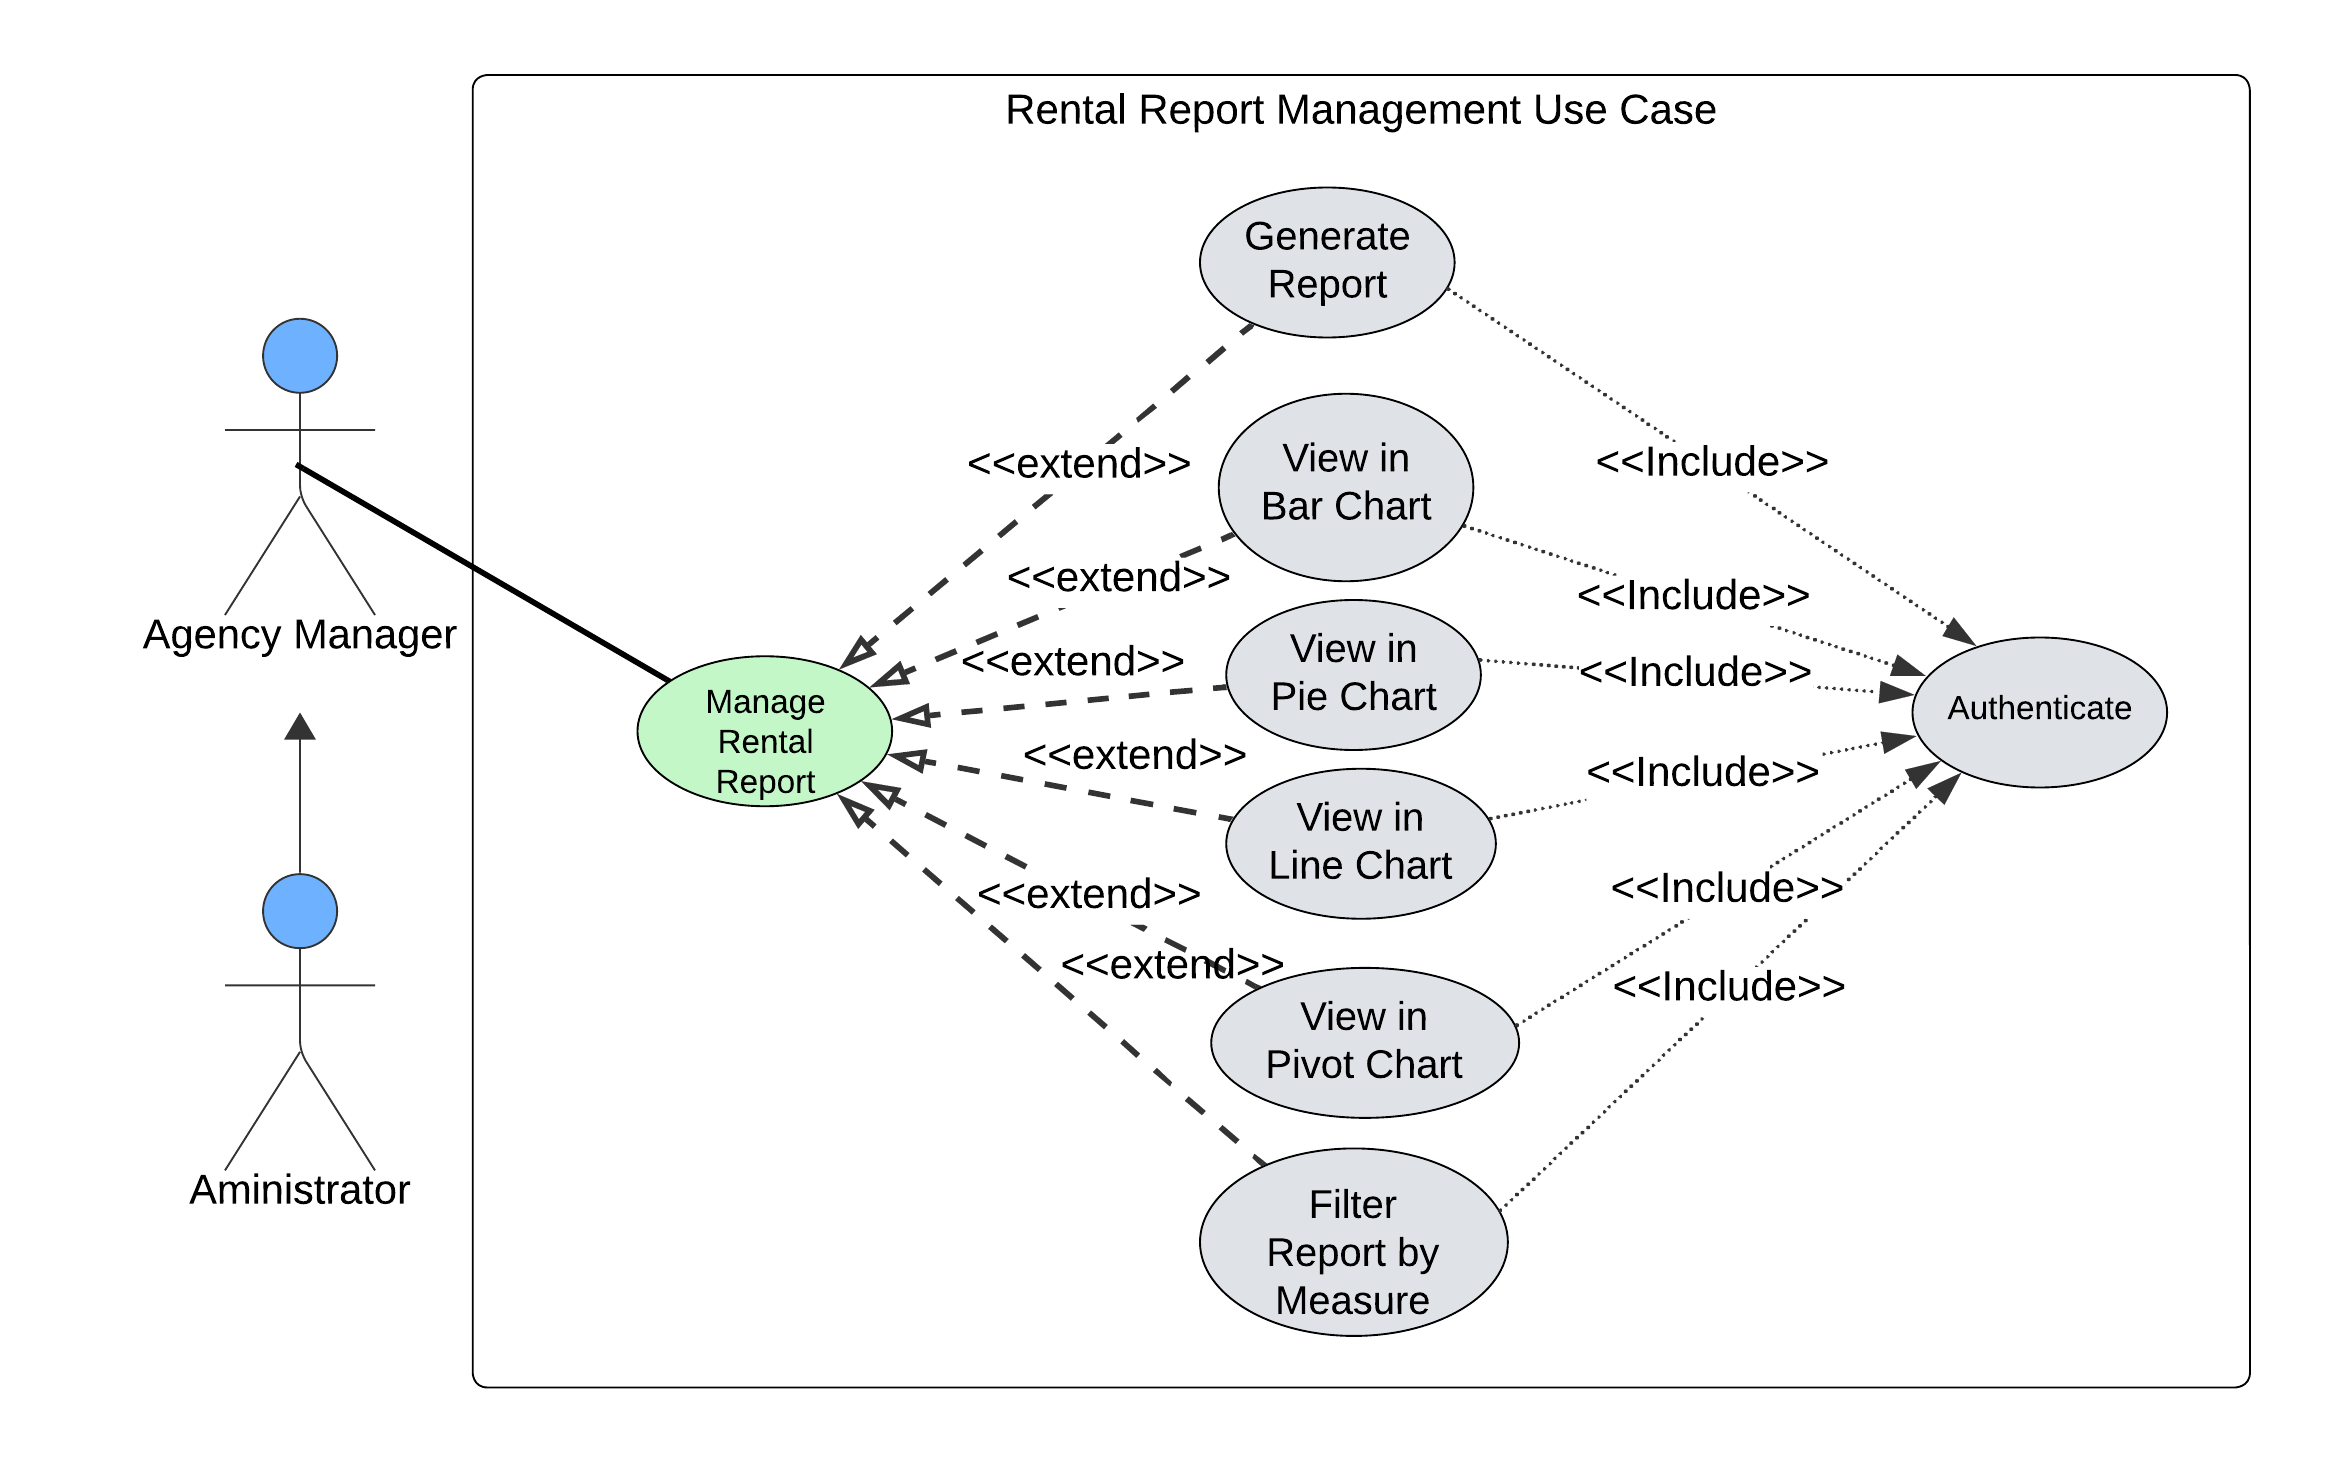
\includegraphics[width=1.2\textwidth]{sprint3/sprint3usecase.png}} % replace with your image path
    \caption{Sprint 3 Use Case Diagram}
    \label{fig:sprint3_use_case_diagram}
\end{figure}

\subsection{Report Management Sequence Diagram}
The sequence diagram below illustrates the process of generating rental order reports:

\begin{itemize}
    \item Administrator selects report generation.
    \item System shows report configuration form.
    \item Administrator picks view mode (bar, pie, line, pivot).
    \item Applies filters (order date, customer, product), generates and displays report, and adjusts as needed.
\end{itemize}
Figure \ref{fig:report_sequence_diagram} illustrates the sequence diagram for the process of generating rental order reports in Sprint 3.

\begin{figure}[h]
    \centering
    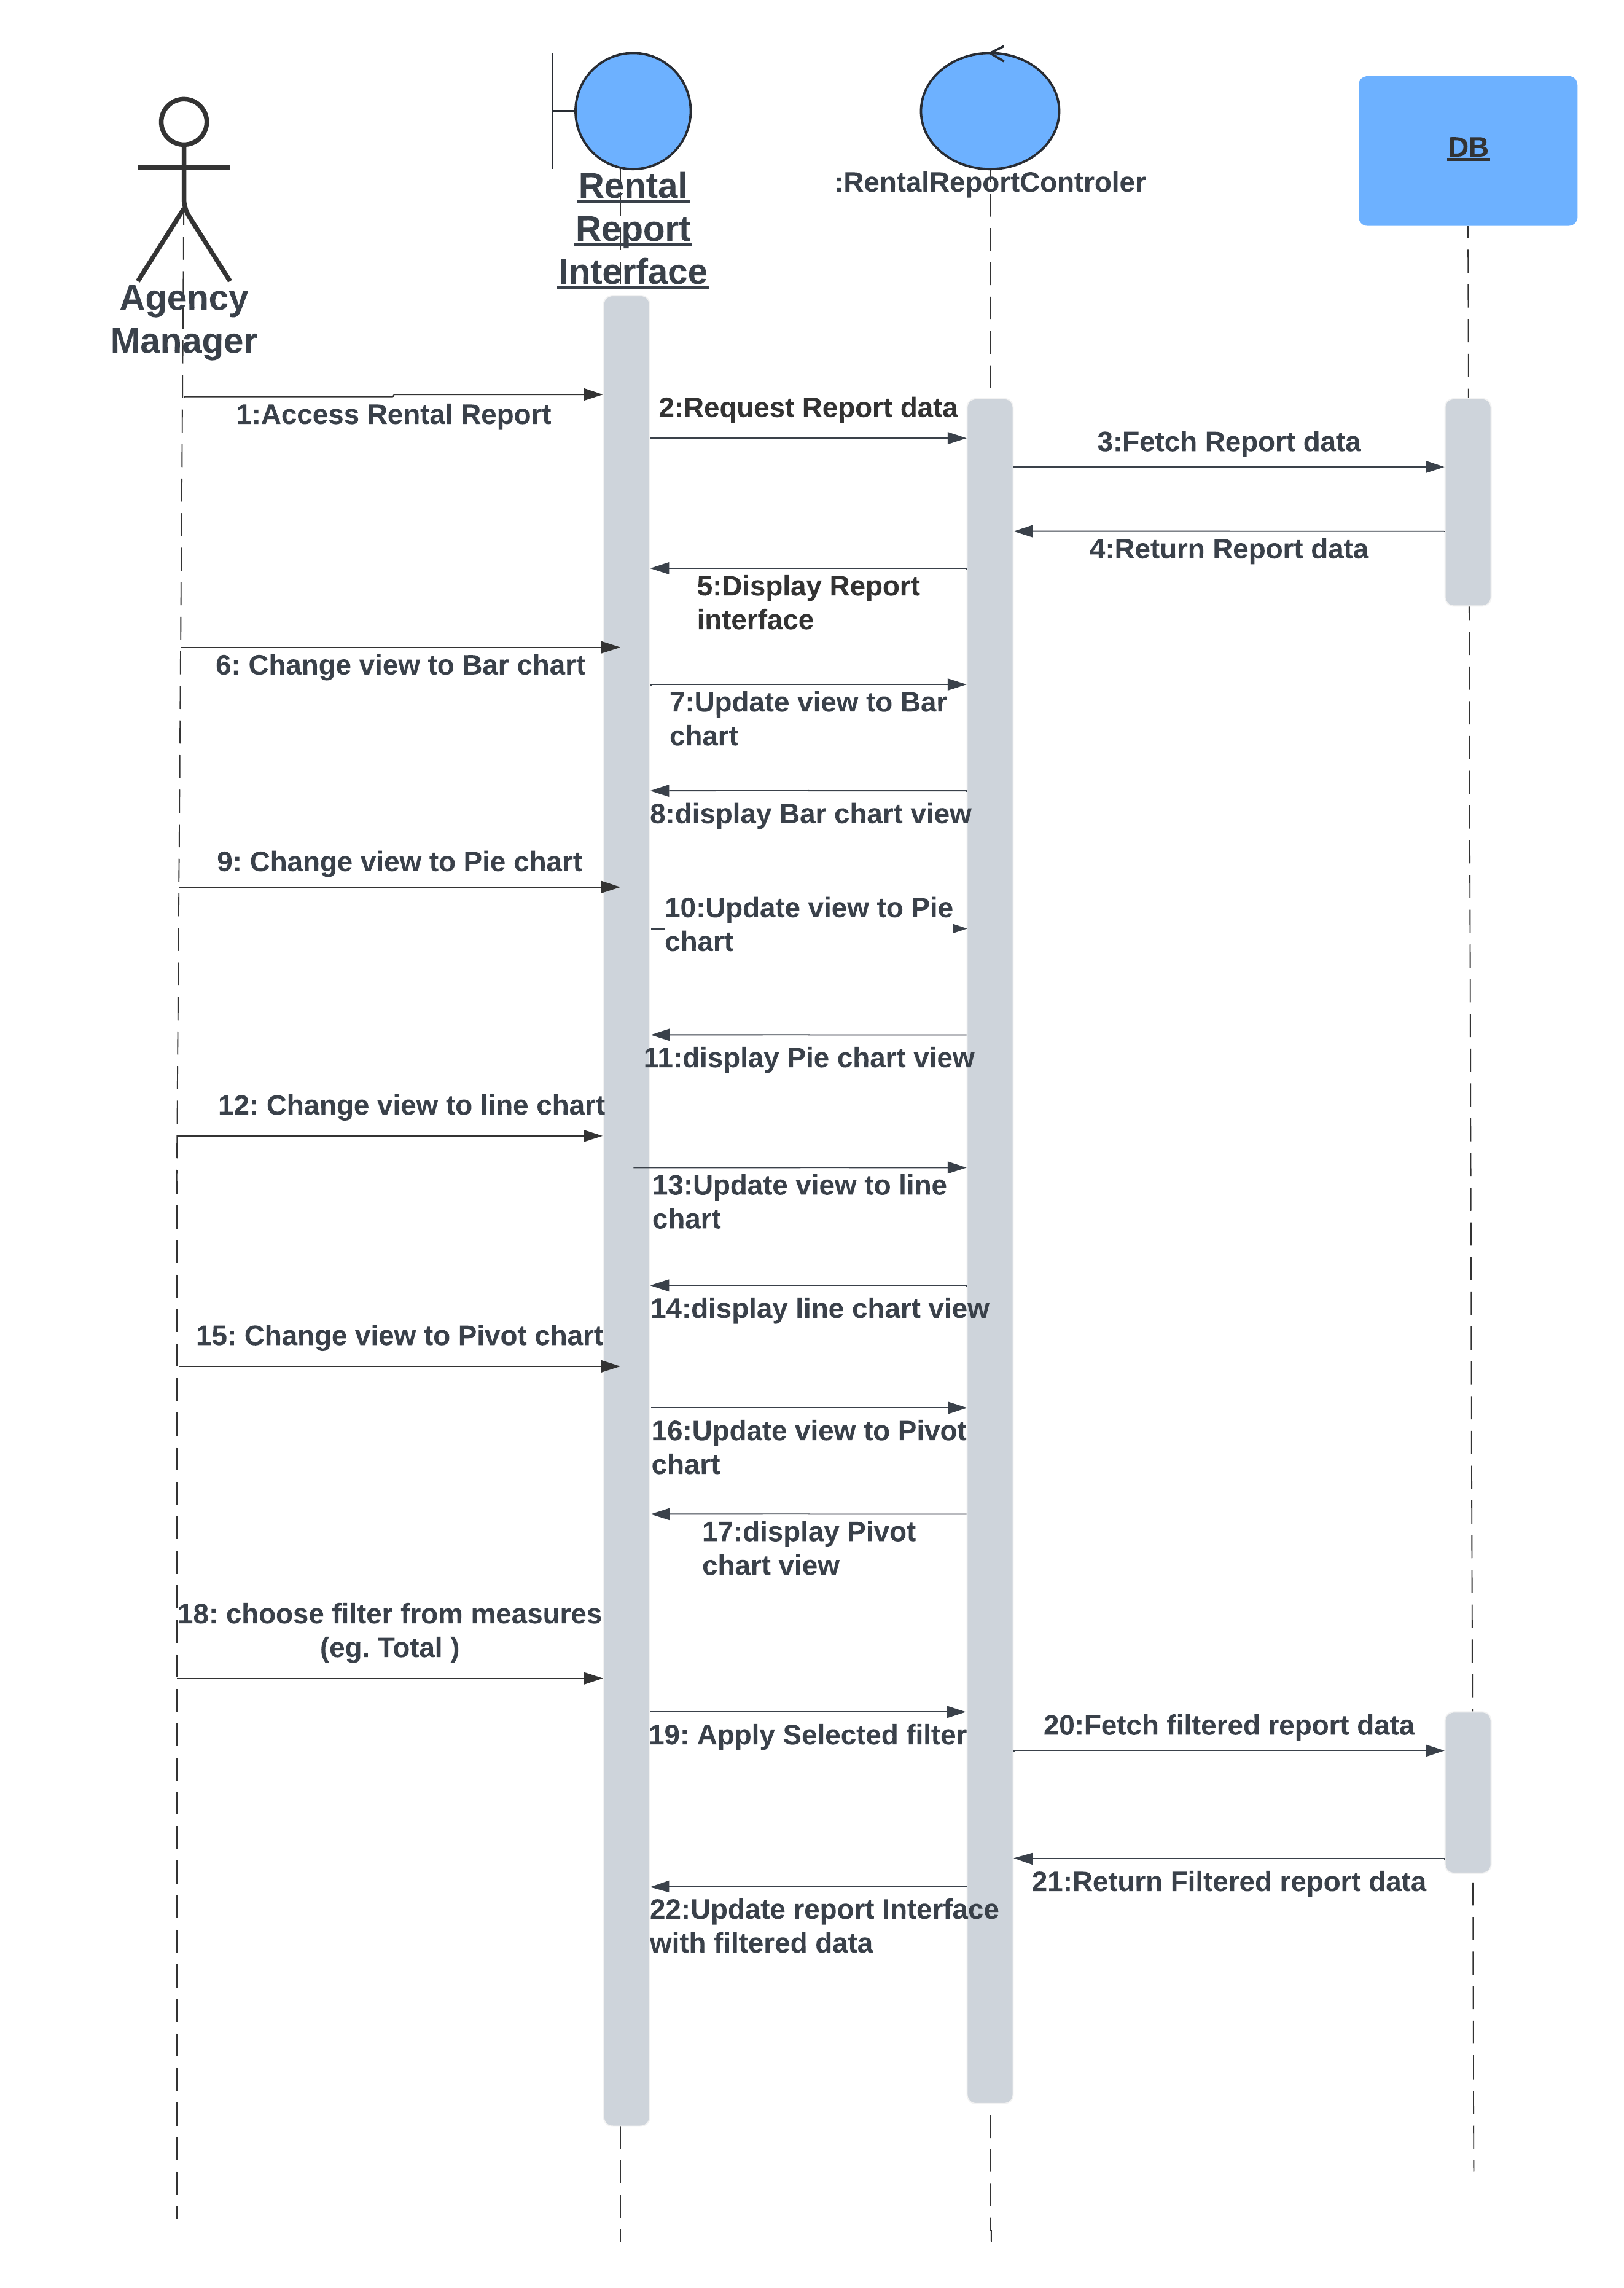
\includegraphics[width=0.7\textwidth]{sprint3/Sprint3Sequence.png} % replace with your image path
    \caption{Sequence Diagram for "Generating Rental Order Reports"}
    \label{fig:report_sequence_diagram}
\end{figure}


\section{Sprint Realization}


\subsection{Bar Chart View}
Figure \ref{fig:bar_chart_view} shows the rental order report in a bar chart format. This view helps in comparing rental orders over different periods.

\begin{figure}[h]
    \centering
    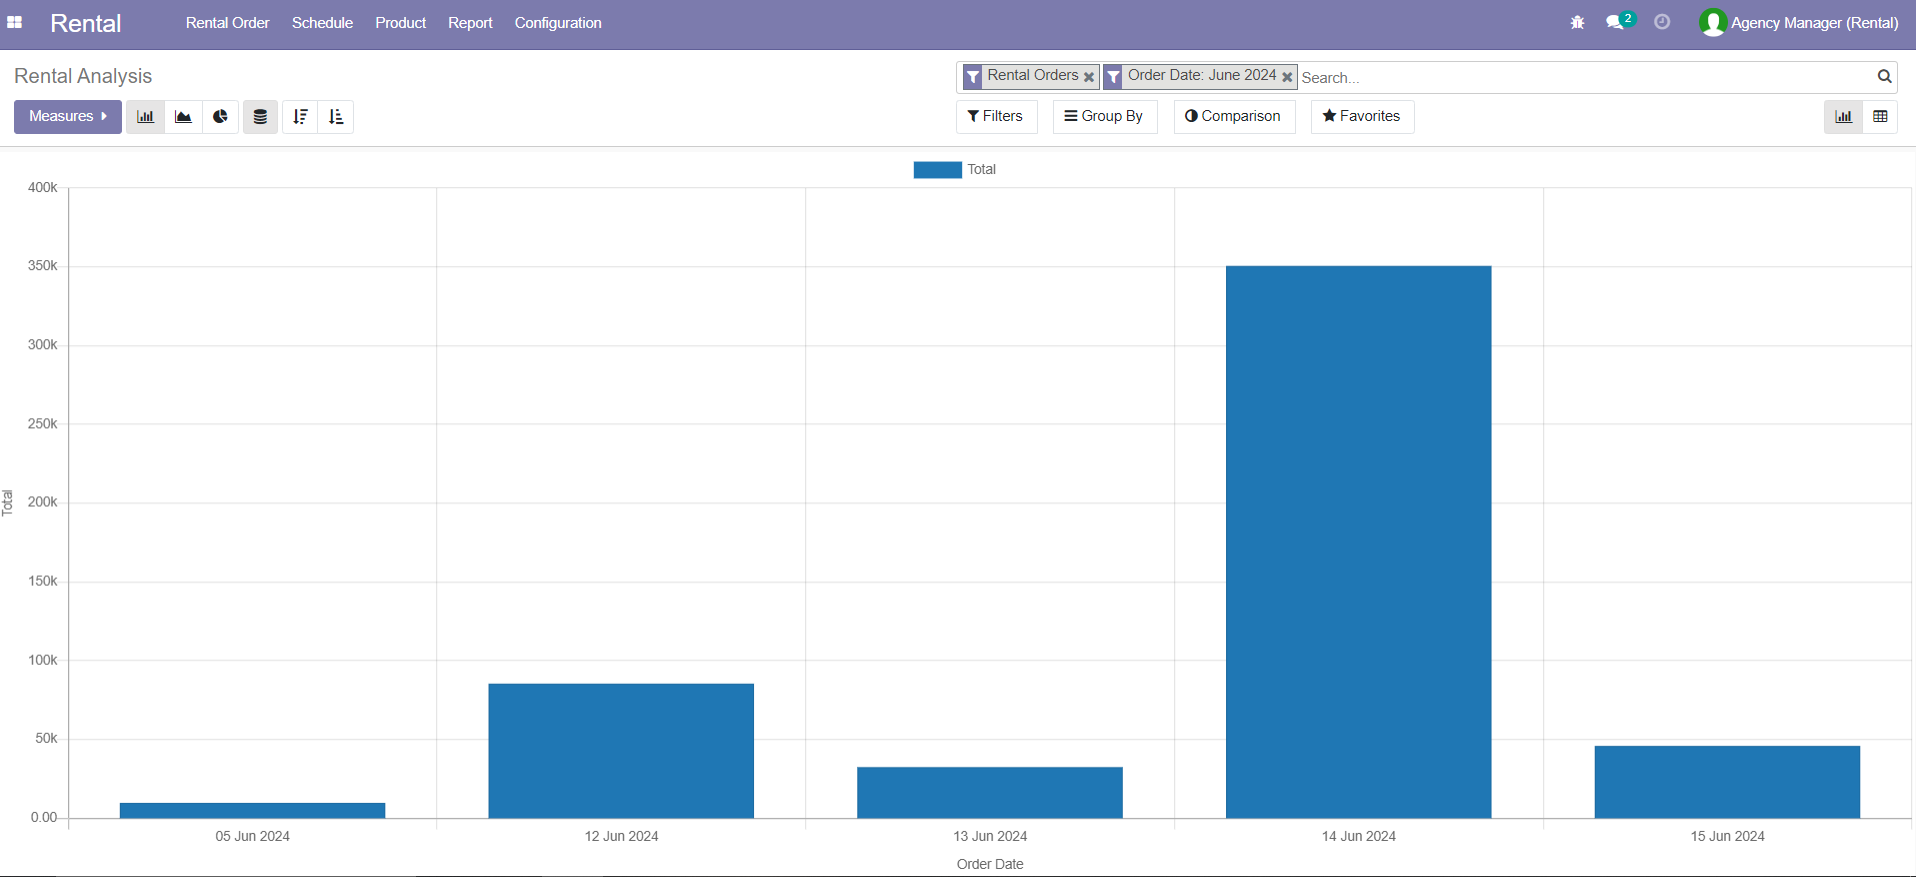
\includegraphics[width=0.8\textwidth]{sprint3/reportbarchart.png} % replace with your image path
    \caption{Screenshot of Rental Order Report - Bar Chart View}
    \label{fig:bar_chart_view}
\end{figure}

\subsection{Pie Chart View}
Figure \ref{fig:pie_chart_view} presents the rental order report in a pie chart format. This view is useful for understanding the distribution of rental orders across different categories.

\begin{figure}[h]
    \centering
    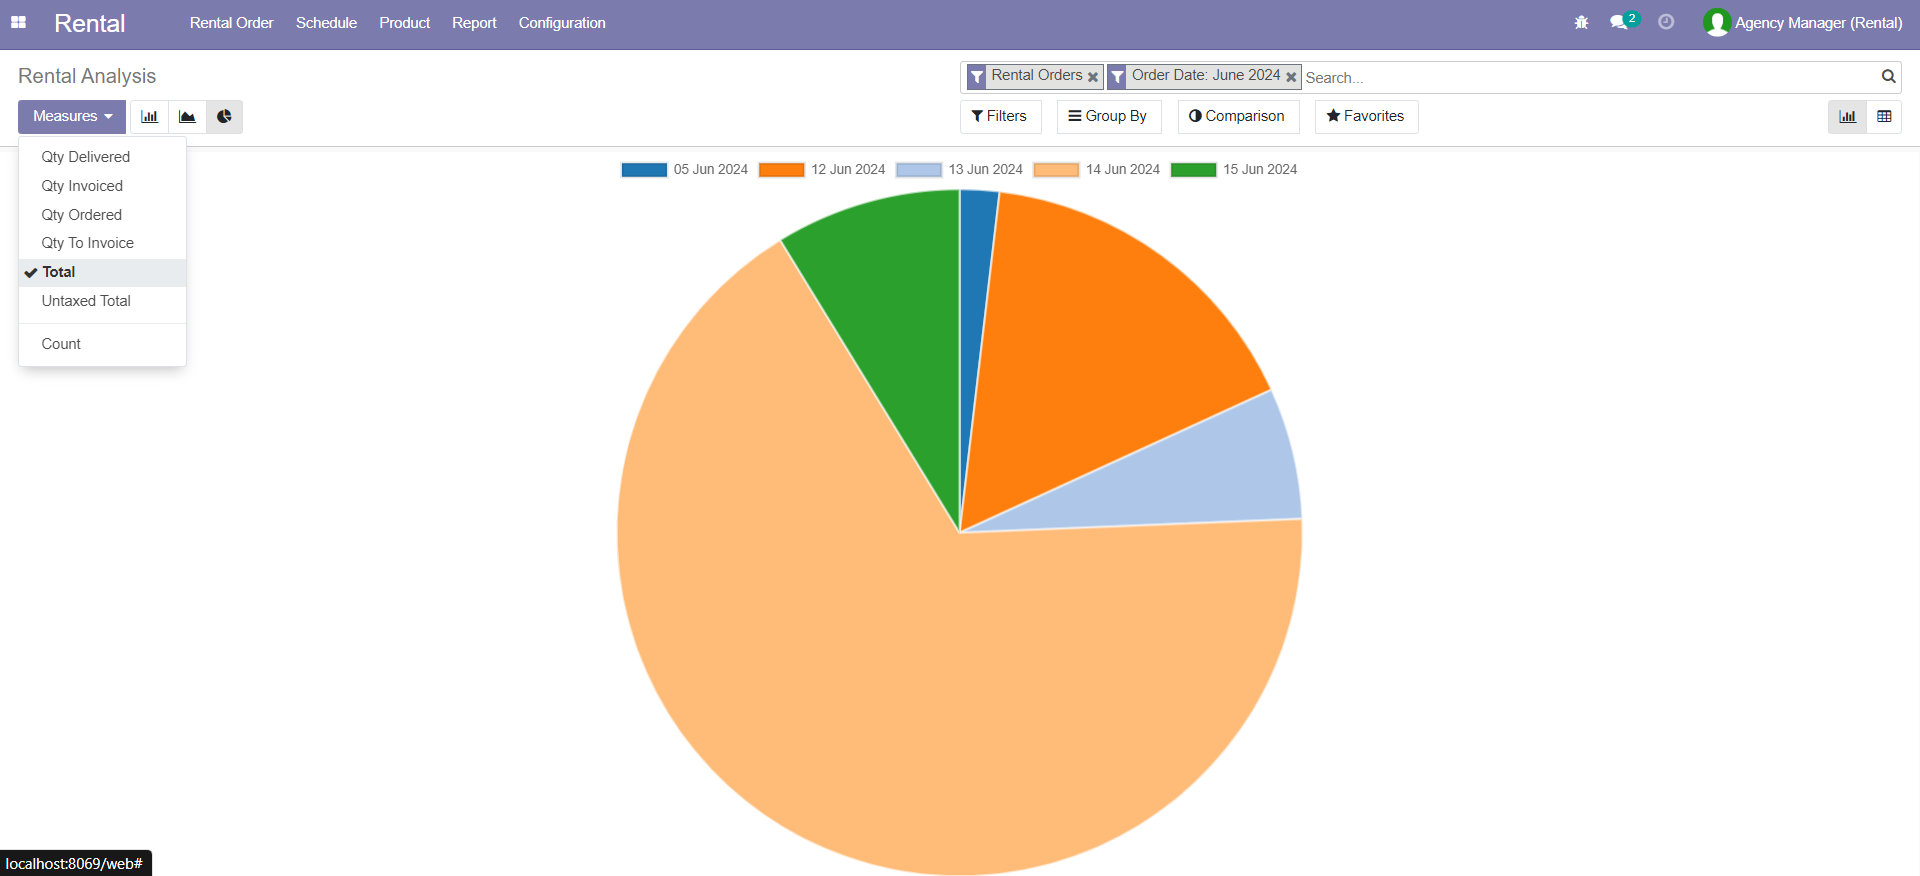
\includegraphics[width=0.8\textwidth]{sprint3/reportpiechart.png} % replace with your image path
    \caption{Screenshot of Rental Order Report - Pie Chart View}
    \label{fig:pie_chart_view}
\end{figure}

\subsection{Line Chart View}
Figure \ref{fig:line_chart_view} displays the rental order report in a line chart format. This view is ideal for observing trends in rental orders over time.

\begin{figure}[h]
    \centering
    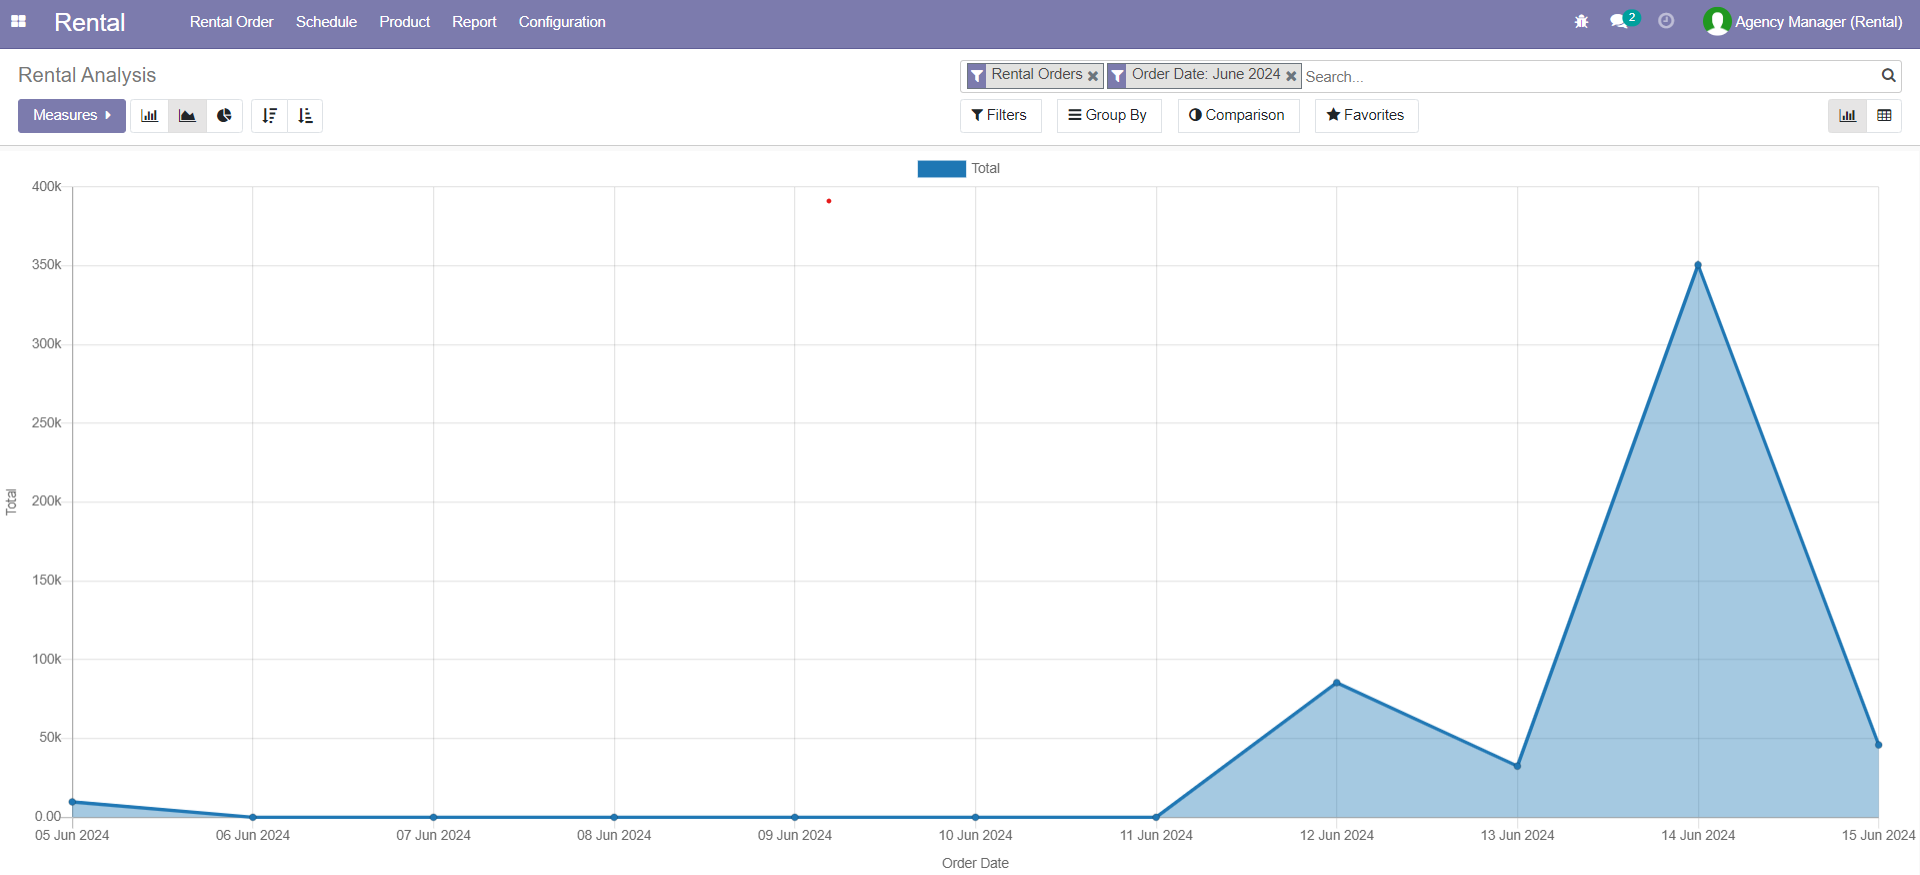
\includegraphics[width=0.8\textwidth]{sprint3/reportlinechart.png} % replace with your image path
    \caption{Screenshot of Rental Order Report - Line Chart View}
    \label{fig:line_chart_view}
\end{figure}

\subsection{Pivot Chart View}
Figure \ref{fig:pivot_chart_view} illustrates the rental order report in a pivot chart format. This view allows for dynamic data analysis and in-depth exploration of rental order details.

\begin{figure}[h]
    \centering
    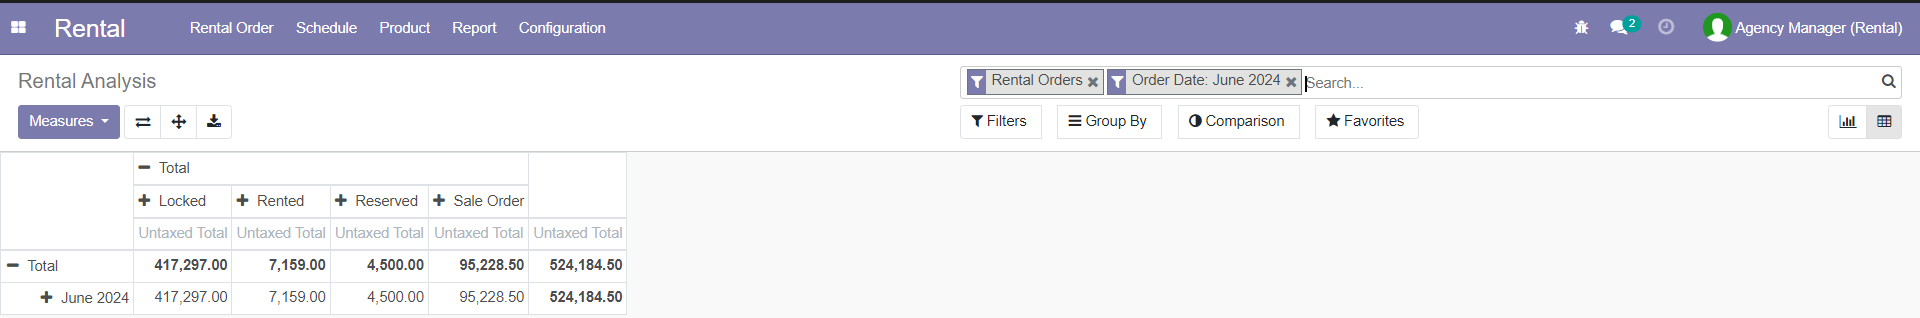
\includegraphics[width=0.\textwidth]{sprint3/reportpivot.png} % replace with your image path
    \caption{Screenshot of Rental Order Report - Pivot Chart View}
    \label{fig:pivot_chart_view}
\end{figure}



\section*{Conclusion}
\addcontentsline{toc}{section}{Conclusion}
In Sprint 3, we enhanced the rental order reporting in Odoo ERP, enabling administrators to generate and analyze reports in various chart formats with dynamic filters. In the next sprint, we will focus on integrating these reporting capabilities with the billing and invoicing module, allowing administrators to manage the system effectively.
.

\chapter{Sprint 4 - Design and implementation}

\section*{Introduction}
\addcontentsline{toc}{section}{Introduction}


In Sprint 4, we focused on the system management capabilities within the Odoo ERP system. This sprint aimed to provide administrators with the ability to manage the system, including app installation, user management, and setting access rights.

\section{Sprint 4 Backlog}
This sprint focuses on enhancing system management capabilities within the Odoo ERP. Table \ref{tab:sprint4_backlog} details the tasks planned for this sprint, outlining their respective durations.
\begin{longtable}{|c|p{8cm}|c|}
    \hline
    \rowcolor{purple!20} \textbf{N°} & \textbf{Tasks} & \textbf{Duration} \\ \hline
    \endfirsthead
    \hline
    \rowcolor{purple!20} \textbf{N°} & \textbf{Tasks} & \textbf{Duration} \\ \hline
    \endhead
    1 & As an administrator, I can install and manage apps. & 4 Day \\ \hline
    2 & As an administrator, I can create, update, and delete user accounts. & 4 Day \\ \hline
    3 & As an administrator, I can manage access rights and permissions for users. & 6 Days \\ \hline
    \caption{Sprint 4 Backlog for System Management}
    \label{tab:sprint4_backlog}
\end{longtable}

\section{Functional Specifications}

\subsection{Use Case Diagram}
This section presents the functional specifications for the System Management module.

Figure \ref{fig:sprint4_use_case_diagram} illustrates the Use Case Diagram specifically designed for Sprint 4.

\begin{figure}[h]
    \centering
    \makebox[\textwidth][c]{%
        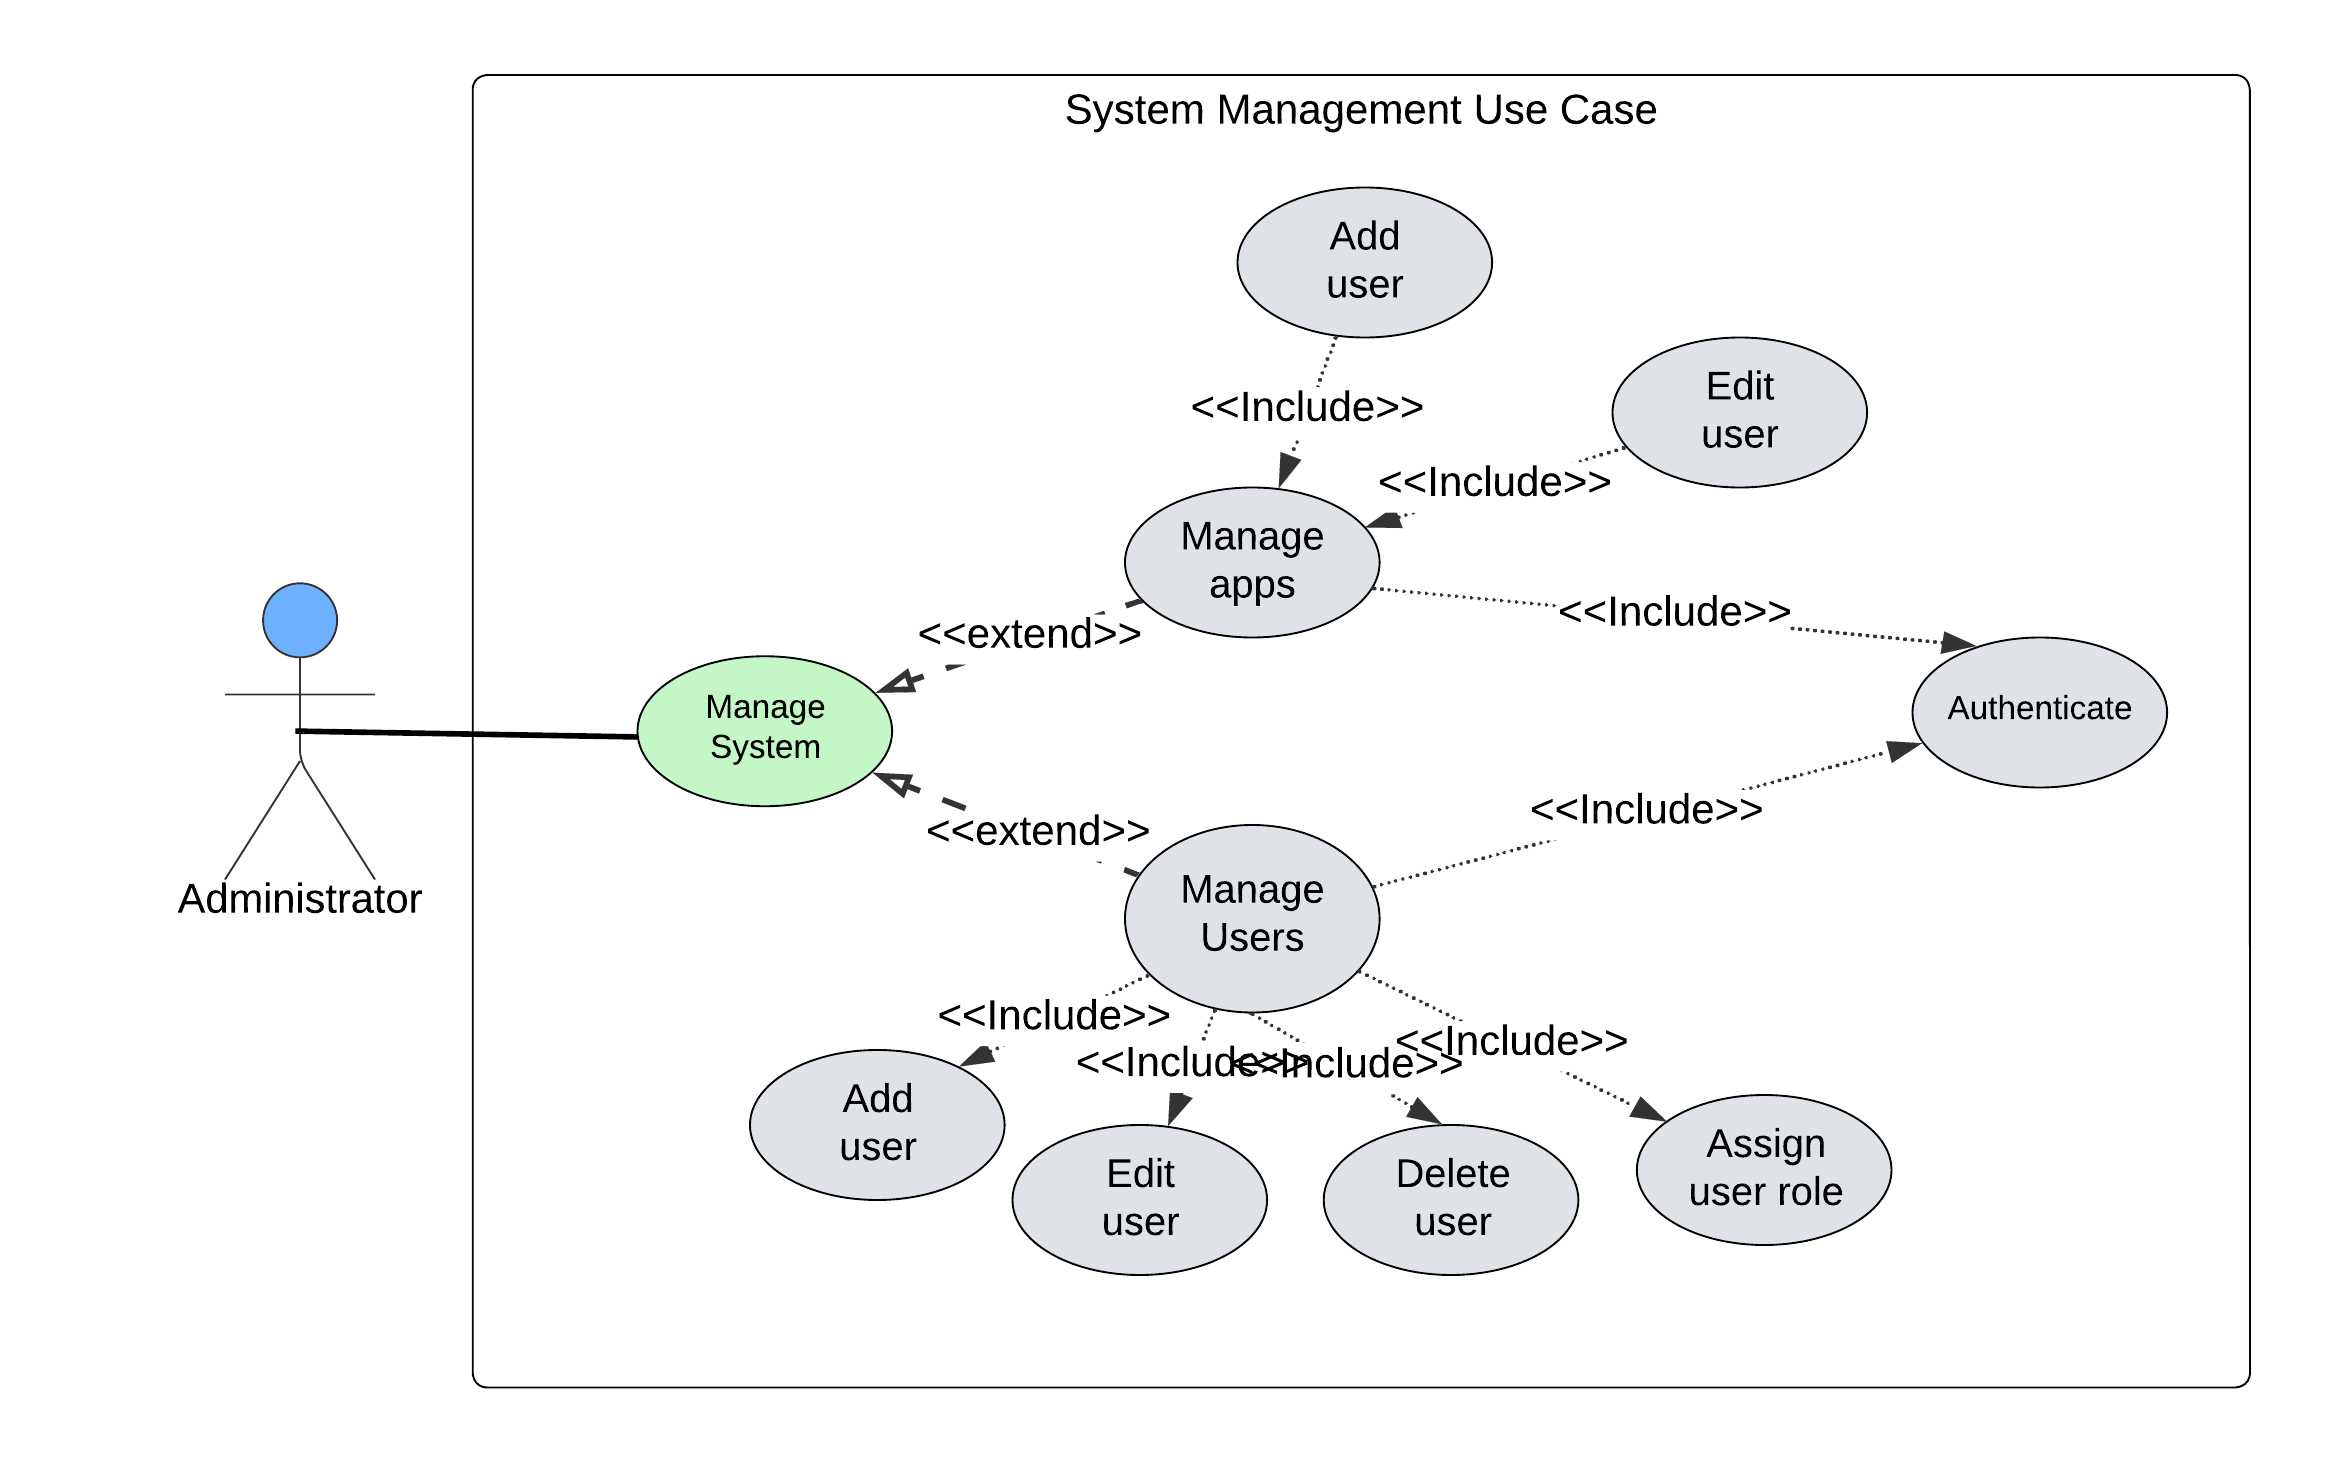
\includegraphics[width=1.2\textwidth]{sprint4/sprint4usecase.png}} % replace with your image path
    \caption{Sprint 4 Use Case Diagram}
    \label{fig:sprint4_use_case_diagram}
\end{figure}

\subsection{System Management Sequence Diagrams}
The sequence diagrams below illustrate the processes of installing an app and managing user accounts.

\begin{itemize}
    \item Administrator installs and manages apps.
    \item Administrator creates, updates, and deletes user accounts.
    \item Administrator sets access rights and permissions.
\end{itemize}

Figure \ref{fig:system_management_sequence_diagram} depicts the Sequence Diagram for managing system functionalities.

\begin{figure}[h]
    \centering
    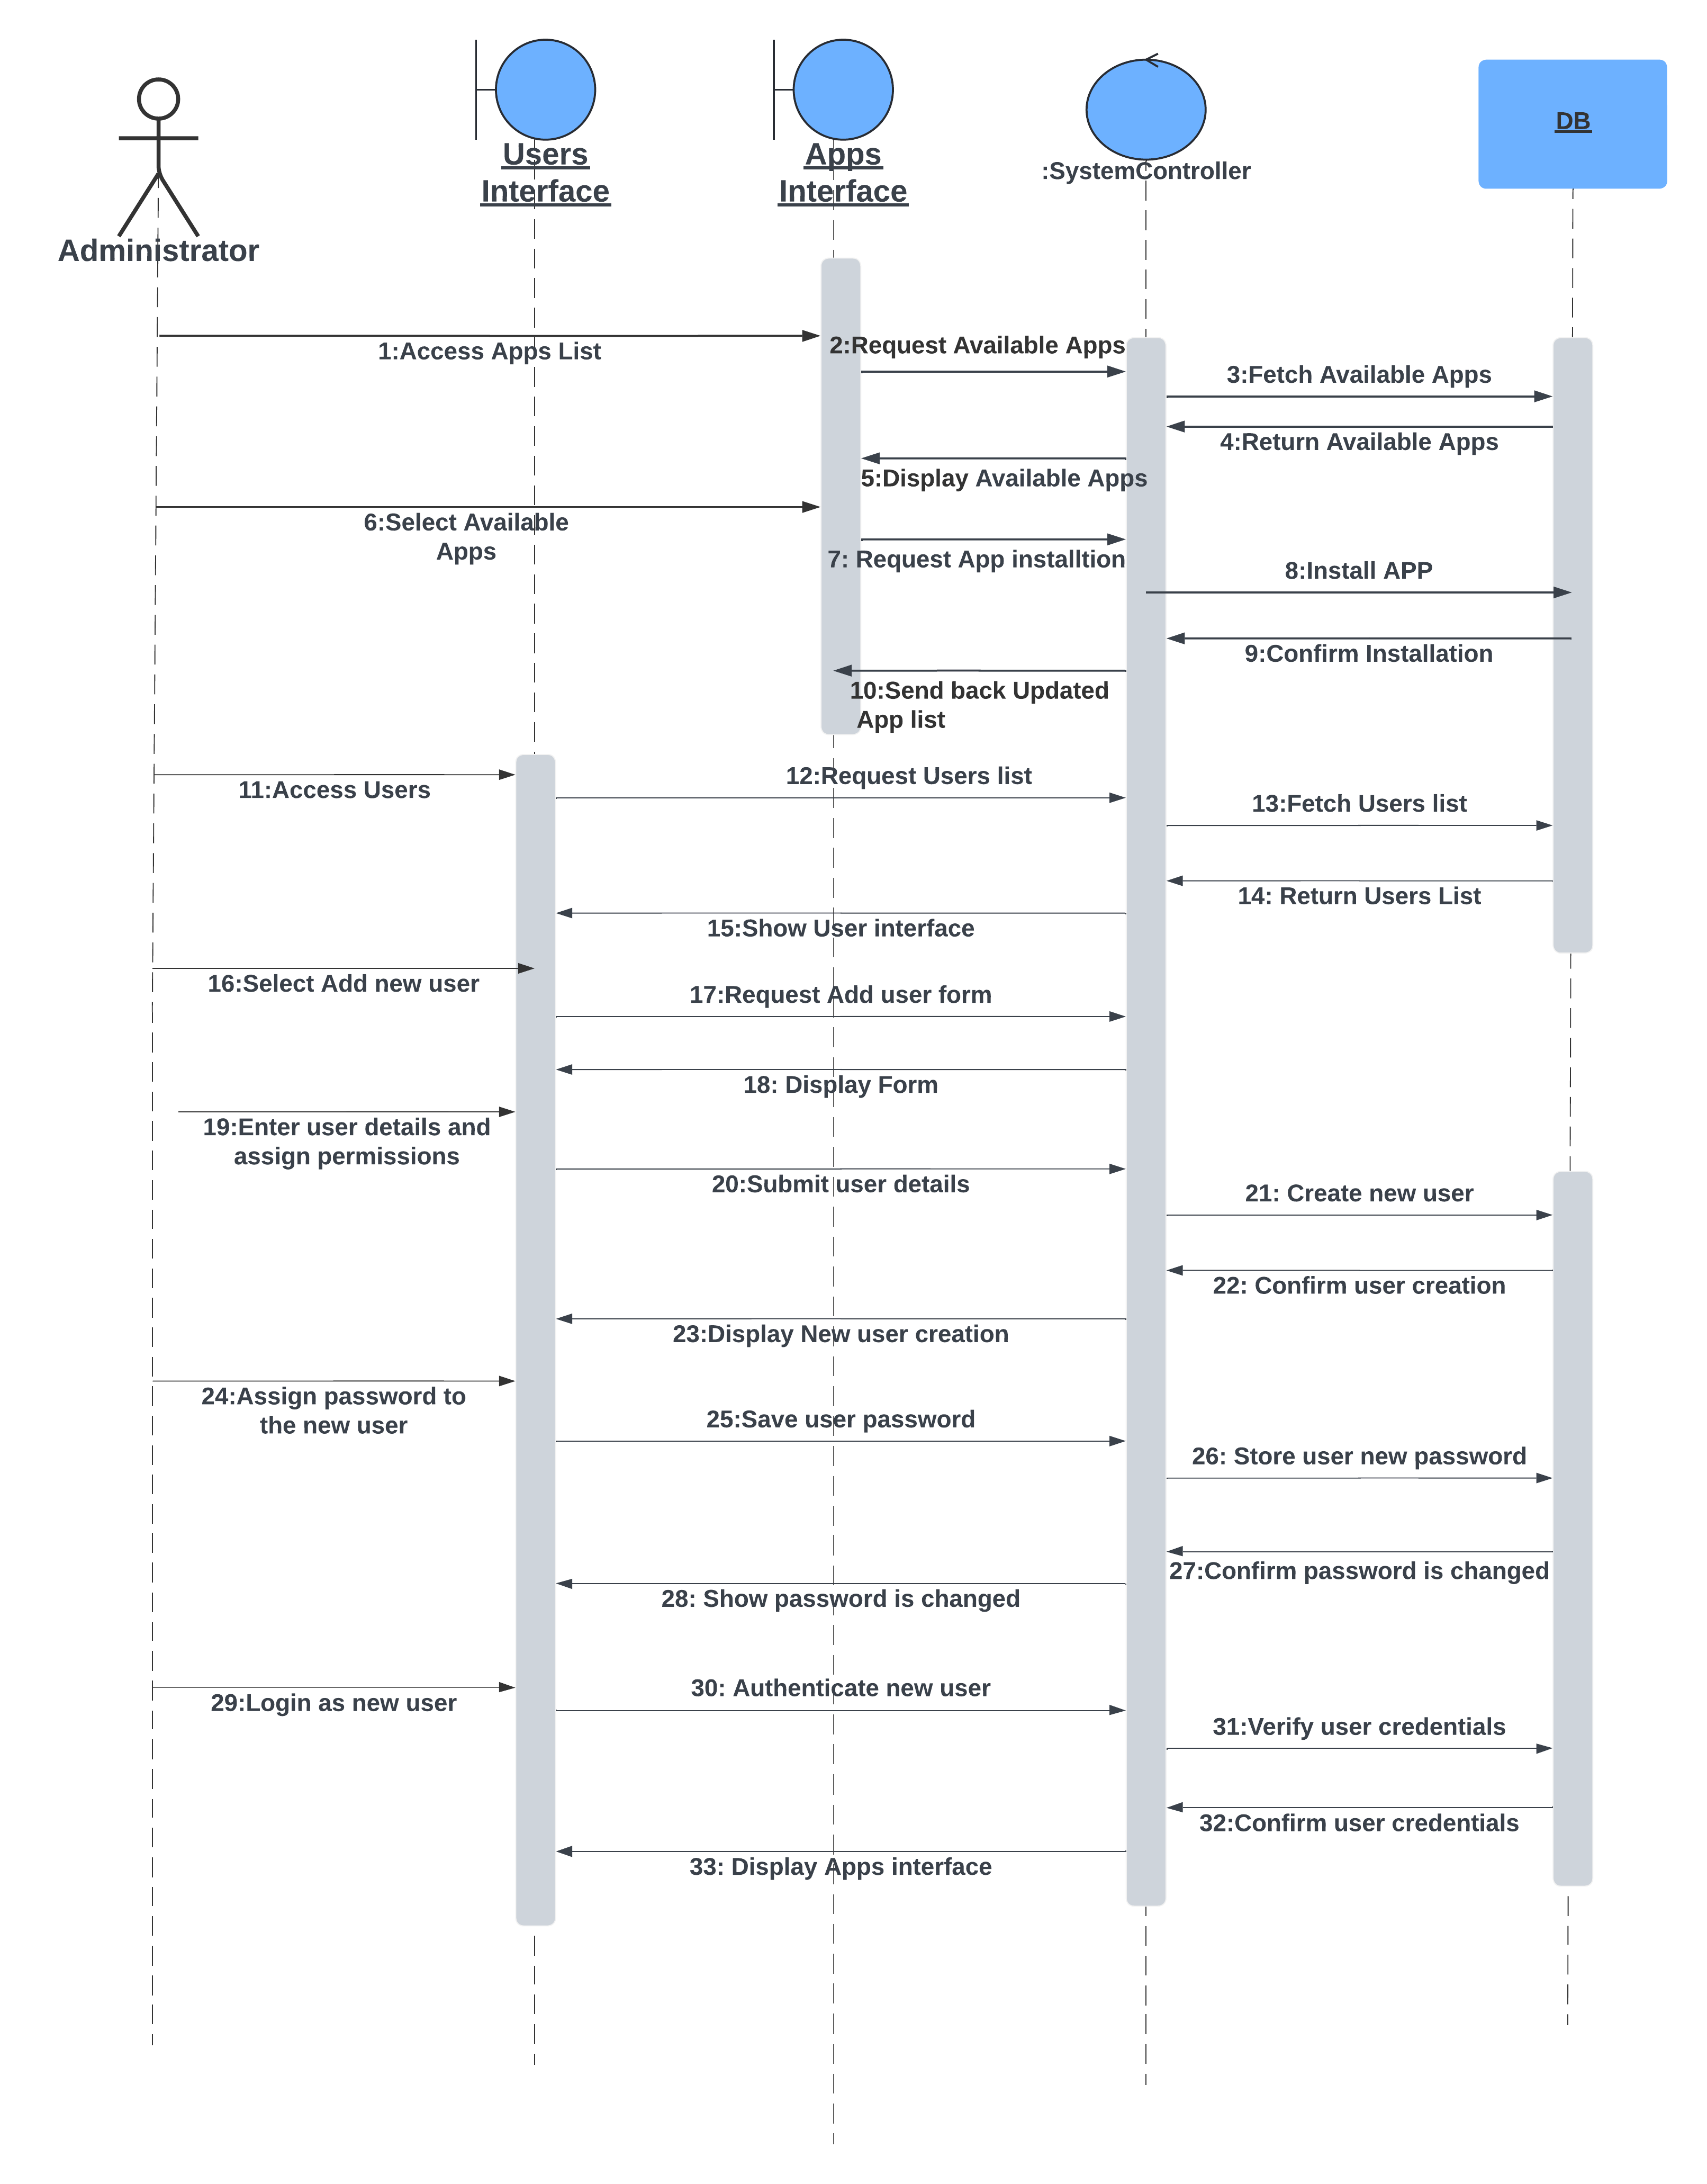
\includegraphics[width=0.7\textwidth]{sprint4/sprint4sequence.png} % replace with your image path
    \caption{Sequence Diagram for "System Management"}
    \label{fig:system_management_sequence_diagram}
\end{figure}
\section{Sprint Realization}

\subsection{System Management Screenshots}
\newpage
\subsection{App Interface}
Figure \ref{fig:app_interface} shows the system app interface where the administrator can upgrade or delete apps.

\begin{figure}[h]
    \centering
    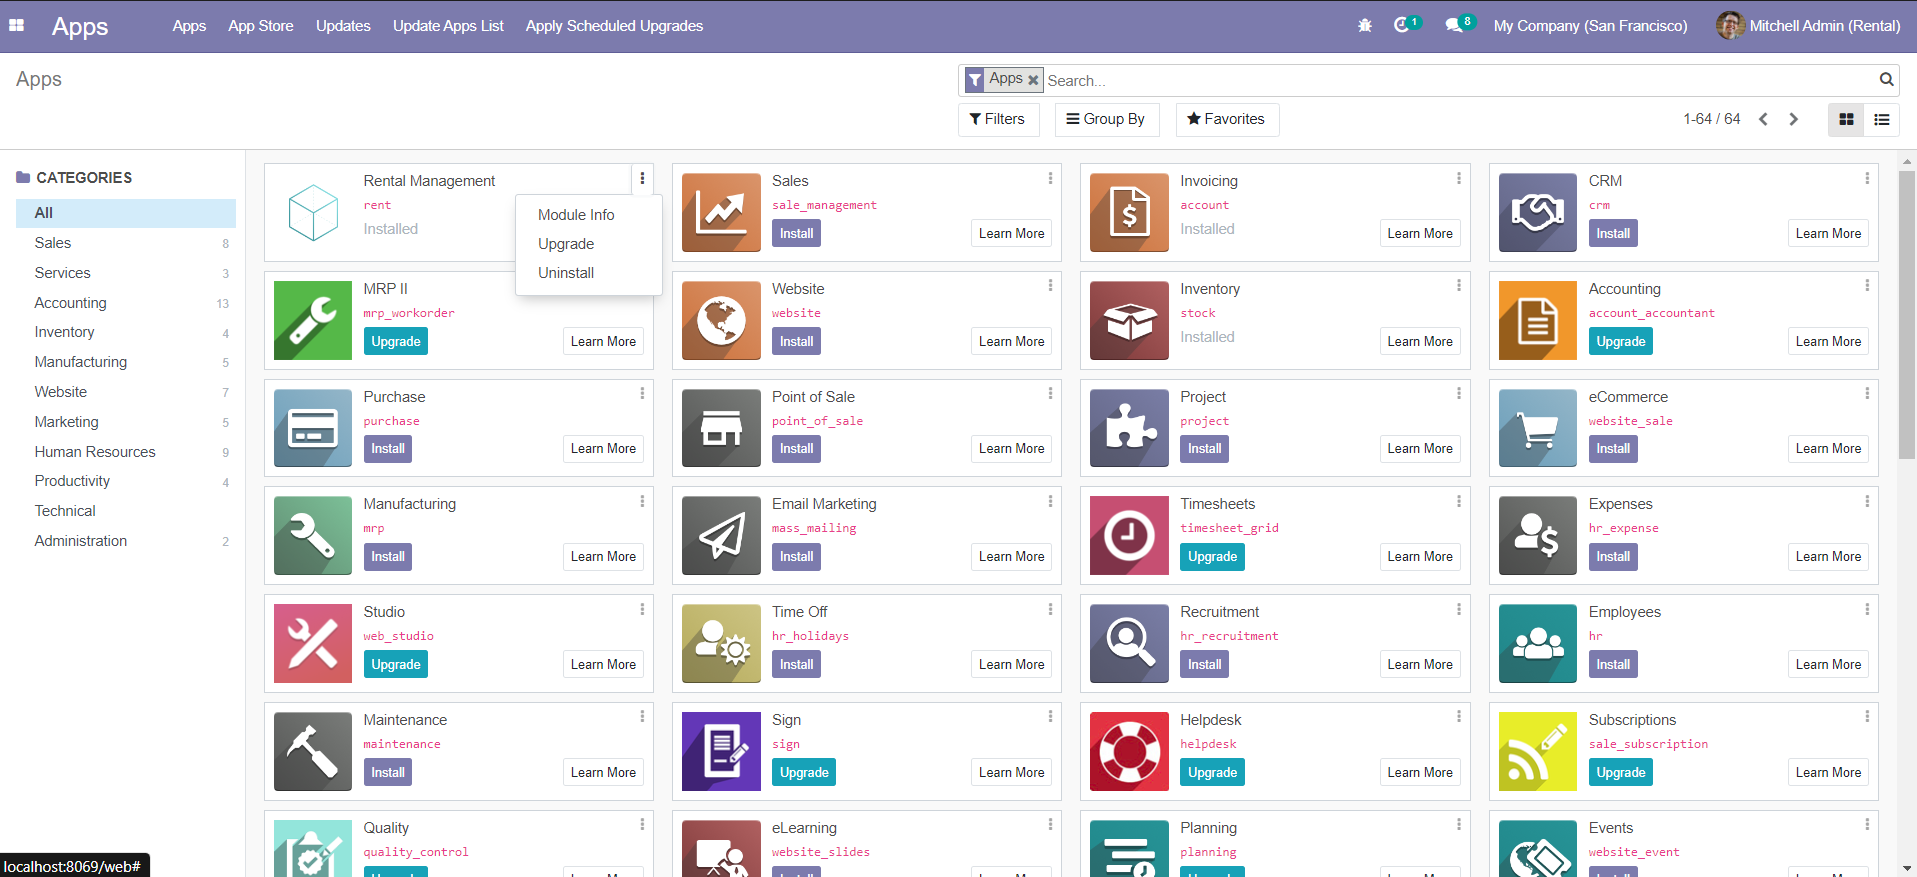
\includegraphics[width=1\textwidth]{sprint4/managesystem1.png} % replace with your image path
    \caption{Screenshot of the App Interface for Administrators}
    \label{fig:app_interface}
\end{figure}

\subsection{User Interface}
Figure \ref{fig:user_interface} presents the user interface showing the basic information of users.

\begin{figure}[h]
    \centering
    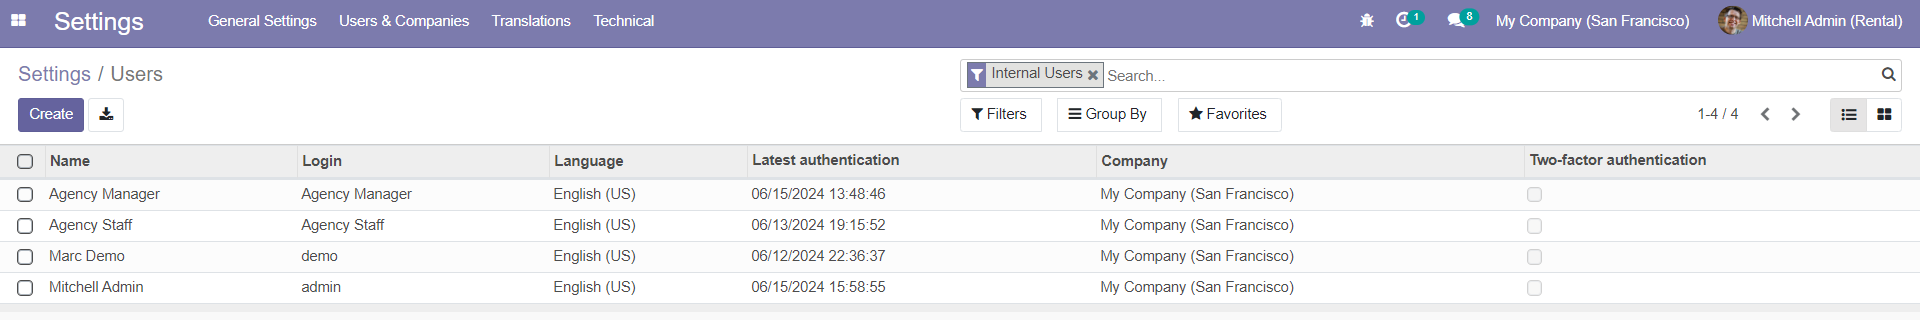
\includegraphics[width=1\textwidth]{sprint4/managesystem2.png} % replace with your image path
    \caption{Screenshot of the User Interface}
    \label{fig:user_interface}
\end{figure}
\newpage
\subsection{Adding a New User}
Figure \ref{fig:add_user_form} shows the form to add a new user, including assigning the right to manage the rental app.

\begin{figure}[h]
    \centering
    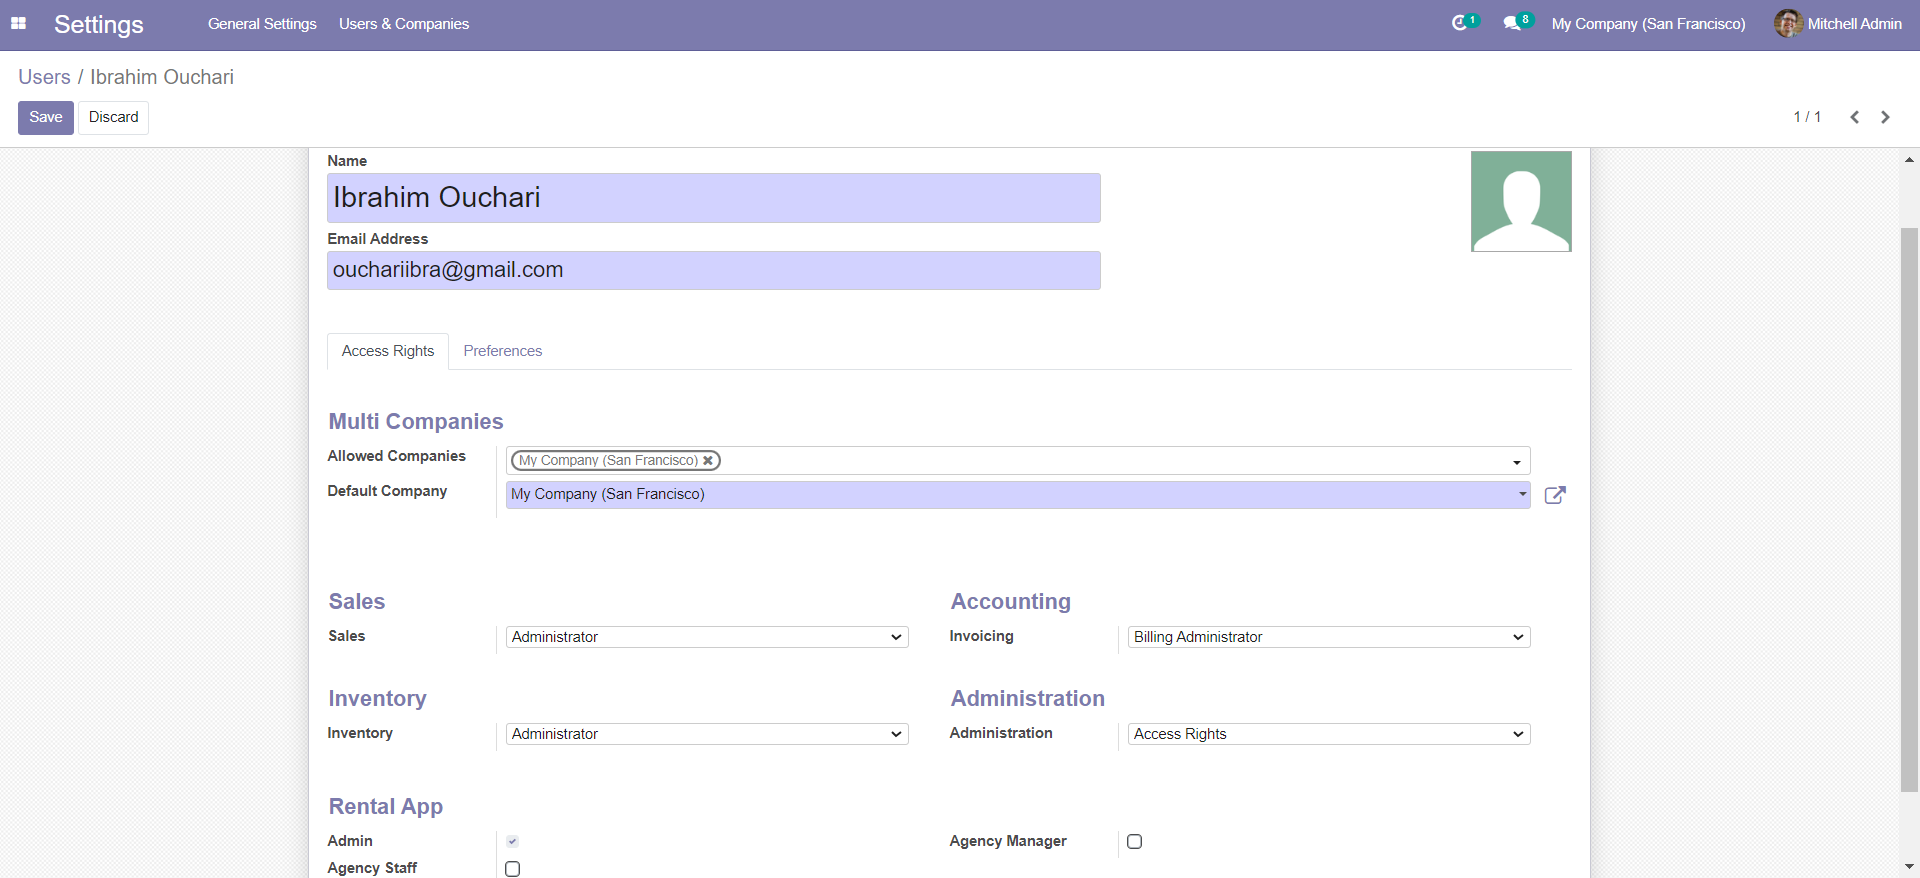
\includegraphics[width=1\textwidth]{sprint4/managesystem3.png} % replace with your image path
    \caption{Filling Out the Form to Add a New User}
    \label{fig:add_user_form}
\end{figure}

\subsection{Assigning a Password}
Figure \ref{fig:assign_password} illustrates the process of assigning a password to the newly created user.

\begin{figure}[h]
    \centering
    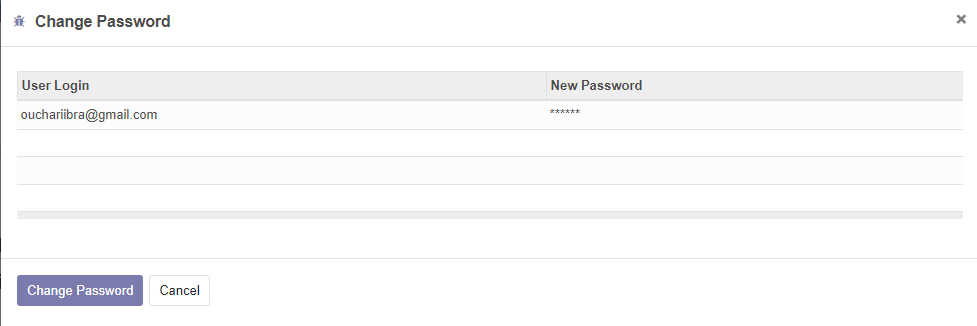
\includegraphics[width=1\textwidth]{sprint4/managesystem4.png} % replace with your image path
    \caption{Assigning a Password to the New User}
    \label{fig:assign_password}
\end{figure}
\newpage
\subsection{Logging In as the New User}
Figure \ref{fig:login_new_user} depicts logging into the app using the newly created account.

\begin{figure}[h]
    \centering
    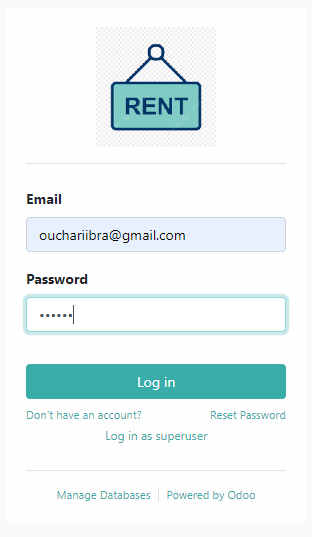
\includegraphics[width=0.2\textwidth]{sprint4/managesystem5.png} % replace with your image path
    \caption{Logging In with the Newly Created Account}
    \label{fig:login_new_user}
\end{figure}

\subsection{User Interface for New Account}
Figure \ref{fig:new_account_interface} shows the interface while using the newly created account.

% \begin{figure}[h]
%     \centering
%     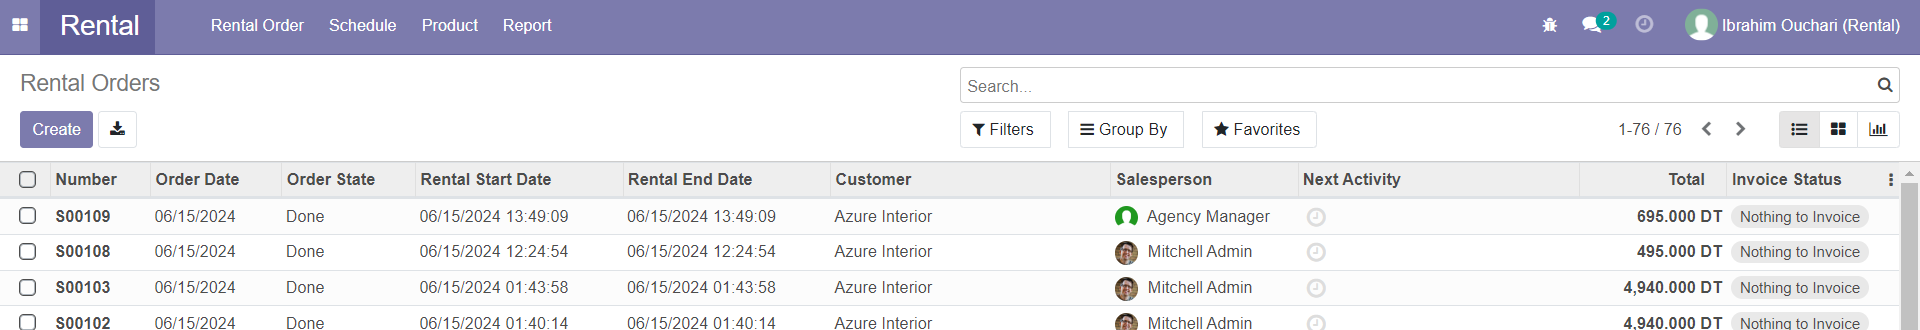
\includegraphics[width=1\textwidth]{sprint4/managesystem6.png} % replace with your image path
%     \caption{User Interface with the Newly Created Account}
%     \label{fig:new_account_interface}
% \end{figure}
\begin{figure}[h]
    \centering
    \makebox[\textwidth][c]{%
        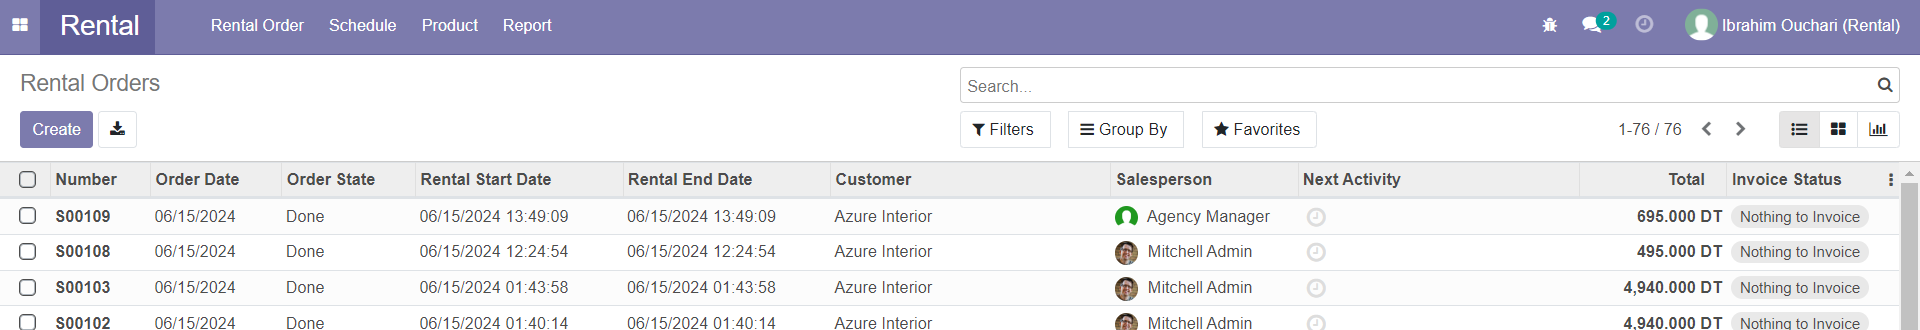
\includegraphics[width=1.2\textwidth]{sprint4/managesystem6.png}} % replace with your image path
    \caption{User Interface with the Newly Created Account}
    \label{fig:new_account_interface}
\end{figure}
\newpage
\section*{Conclusion}
\addcontentsline{toc}{section}{Conclusion}

In Sprint 4, we focused on enhancing the system management capabilities in Odoo ERP, allowing administrators to install and manage apps, create and manage user accounts, and set access rights and permissions. These functionalities enable efficient system management. The next sprint will continue to refine these capabilities and ensure smooth integration with other modules.

\chapter{Realisation}
\section{Introduction}

In this chapter, we present the working environment that allowed us to develop our application initially. Then we present the deployment diagram.

\section{Technical Environment}

The technical architecture, often also called computer architecture or software architecture, represents the overall structure of a computer system, including hardware, software, network protocols, standards used, as well as the physical and logical aspects of interactions and relationships between these different elements.

\subsection{Hardware Choices}

In this part, we mention the hardware(s) that we used to complete the work as shown in the table below (see Table \ref{tab:hardware-choices}).
\begin{table}[htbp]
    \centering
    
    \begin{tabular}{|p{2cm}|p{3cm}|p{2cm}|p{4cm}|p{2cm}|}
        \hline
        \rowcolor{purple!20} % Light green background
        Device(s) & Processor & Memory & Storage & OS \\
        \hline
        Machine & & & & \\
        Lenovo Ideapad 320  & Intel Core i3 6006u & 8 GB & 500 GB SSD and  1 TB HDD & Windows 10\\
        \hline
       \end{tabular}
       \caption{Hardware Choices}
    \label{tab:hardware-choices}
\end{table}

\subsection{Software Choices}

In this part, we detail the different tools used for configuration and development of our application.


\begin{table}[h]
    \centering
    
    \begin{tabular}{|c|c|c|}
        \hline
       \raisebox{1.3\height}{
\includegraphics[width=0.2\textwidth]{media/odoo_logo.png}} &
        
\includegraphics[width=0.2\textwidth]{media/pycharm_logo.png} &
        
\includegraphics[width=0.2\textwidth]{media/vscode.png} \\
        
        \hline
        \textbf{\cellcolor{gray!50}Odoo} & \textbf{\cellcolor{gray!50}PyCharm} & \textbf{\cellcolor{gray!50}Vscode} \\
        \hline
    \end{tabular}
    \caption{Software Used}
    \label{tab:Software Used}
\end{table}
• \textbf{Odoo} \cite{odoo}: A comprehensive suite of business applications, including CRM, e-commerce, billing, and inventory management. Odoo is highly modular and user-friendly, facilitating rapid application development and customization.

• \textbf{PyCharm} \cite{pycharm}: A Python IDE providing code analysis, debugging, unit testing, VCS integration, and Django support. PyCharm enhances productivity and code quality with its powerful features.

• \textbf{Visual Studio Code (VSCode)} \cite{vscode}: A free source-code editor for Windows, Linux, and macOS by Microsoft. It supports debugging, syntax highlighting, code completion, refactoring, and Git integration. VSCode is highly customizable with extensions.
\newpage
\subsection{Database Management System}

\begin{figure}[h]
    \centering
    
\includegraphics[width=0.5\textwidth]{media/PostgreSQL-Logo.wine.png}
    \caption{Database Management System}
    \label{fig:dbms}
\end{figure}

• \textbf{PostgreSQL}\cite{postgresql}: PostgreSQL is a powerful, open-source object-relational database management system (ORDBMS) capable of safely handling the most complex data workloads. It has several user interfaces, such as PSQL for command-line interaction and PgAdmin as a graphical administration tool.




\subsection{Programming Languages}



\begin{table}[h]
    \centering
    
    \begin{tabular}{|c|c|c|}
        \hline
        
\includegraphics[width=0.15\textwidth]{media/xml_logo.png} &
        \includegraphics[width=0.2\textwidth]{media/python_logo.png} &
        \includegraphics[width=0.2\textwidth]{media/css-3.png} \\
        \hline
        \textbf{\cellcolor{gray!50}XML} & \textbf{\cellcolor{gray!50}Python} & \textbf{\cellcolor{gray!50}CSS} \\
        \hline
    \end{tabular}
    \caption{Programming Languages}
    \label{tab:programming-languages}
\end{table}
\newpage

\subsection{Tools}


\begin{table}[htbp]
    \centering
   
    \begin{tabular}{|c|c|c|}
        \hline
        \includegraphics[width=0.2\textwidth]{media/drawio.png} &
        \includegraphics[width=0.2\textwidth]{media/PgAdmin4.jpg} &
        \includegraphics[width=0.2\textwidth]{media/git.png} \\
        
        \hline
        \textbf{\cellcolor{gray!50}Drawio} & \textbf{\cellcolor{gray!50}PgAdmin4} & \textbf{\cellcolor{gray!50}git} \\
        \hline
    \end{tabular}
     \caption{Tools}
    \label{tab:Tools}
\end{table}

\begin{itemize}
    \item \textbf{Draw.io} \cite{drawio}: An online tool for creating diagrams, flowcharts, and visual representations. It is user-friendly and supports collaborative work.
    
    \item \textbf{PgAdmin 4} \cite{pgadmin}: A graphical tool for managing PostgreSQL databases, running SQL queries, and visualizing data.
    
    \item \textbf{Git} \cite{git}: A version control system for tracking code changes and managing branches. Essential for collaboration and code management.
\end{itemize}

\subsection{Platform}
\begin{table}[htbp]
    \centering
  
    \begin{tabular}{|c|}
        \hline
        \includegraphics[width=0.2\textwidth]{media/github.png} \\
        \hline
        \textbf{\cellcolor{gray!50}GitHub \cite{github}} \\
        \hline
    \end{tabular}
      \caption{Platform}
    \label{tab:Platform}
\end{table}
\begin{itemize}
    \item \textbf{GitHub}: A web-based platform for version control and collaboration, allowing developers to manage and share their code repositories, track changes, and work on projects collaboratively with features such as pull requests, issues, and project boards.
\end{itemize}



\section*{Conclusion}
\addcontentsline{toc}{section}{Conclusion}


In this chapter, we explore the tools and technologies used in the development of the Odoo application. By leveraging \textbf{Odoo}, we facilitated the creation and customization of business applications. \textbf{PyCharm} was instrumental in enhancing our productivity with its robust Python IDE features, while \textbf{Visual Studio Code} provided a versatile and customizable coding environment. Tools such as \textbf{Drawio} for diagramming, \textbf{PgAdmin 4} for database management, and \textbf{GitHub} for version control and collaboration played a crucial role in ensuring smooth project execution and management. Together, these tools and technologies enabled the efficient and effective development of a comprehensive and modular Odoo application, \\ demonstrating the synergy of modern development practices and tools.



\chapter*{General Conclusion And Perspective}
\addcontentsline{toc}{chapter}{General Conclusion And Perspective}
During this internship, we embarked on a journey of significant learning experiences. We began by understanding the project context and identifying our system's diverse requirements. Through collaborative team discussions, we meticulously planned our work schedule, prioritizing our needs accordingly.

Our final project focused on designing and developing a solution tailored for managing an association. This manuscript comprehensively details each step taken to achieve our anticipated results. Adopting the Scrum methodology, we incrementally built our application, ensuring iterative progress.

Today, the application stands ready for use, successfully meeting our set objectives. Engaging with the research community allowed us to advance across various domains, particularly in development.

We are pleased with the achievements during this internship, having fulfilled all major goals. Our exposure to Scrum methodology and Python programming with Odoo has been invaluable.

Looking ahead, our journey continues as we aim to expand the application's capabilities, including the addition of reporting functionalities. Furthermore, our next step involves developing a website to integrate e-commerce functionalities seamlessly.

In conclusion, this internship provided a platform to apply academic, professional, and interpersonal skills to an engaging topic. We have gained valuable insights into enterprise development, laying a solid foundation for future endeavors.


\thispagestyle{empty}

% After the conclusion, make all pages empty (no headers, footers, or page numbers)
\pagestyle{empty}

% Print bibliography and include it in the TOC
\cleardoublepage
\pagestyle{empty} % Ensure no headers, footers, or page numbers
\printbibliography[heading=bibintoc]
\thispagestyle{empty} % Apply to the current page

% Include annex
\cleardoublepage
\pagestyle{empty} % Ensure no headers, footers, or page numbers
\thispagestyle{empty} 
\chapter*{\centering Annex 1: Odoo System Overview}
\addcontentsline{toc}{chapter}{Annex 1: Odoo System Overview}
\thispagestyle{empty} 
\textbf{Odoo System Architecture}

Odoo's architecture comprises three main components:

\begin{itemize}
\item \textbf{PostgreSQL Database Server:}
  \begin{itemize}
  \item \textbf{Functionality:} Manages data persistence using an Object Relational Mapping (ORM) layer.
  \item \textbf{Role:} Stores and retrieves structured data necessary for the application's operation.
  \item \textbf{Integration:} Seamlessly integrates with other components to ensure data consistency and reliability.
  \end{itemize}
  
\item \textbf{Application Server:}
  \begin{itemize}
  \item \textbf{Functionality:} Contains business logic, work engine, and output generation.
  \item \textbf{Role:} Executes business processes, calculations, and operations defined by the user and application modules.
  \item \textbf{Scalability:} Scales horizontally to handle increased workload and user interactions.
  \end{itemize}
  
\item \textbf{Presentation Server:}
  \begin{itemize}
  \item \textbf{Functionality:} Allows user access through any web browser (e.g., Chrome, Firefox).
  \item \textbf{Role:} Renders user interfaces, forms, reports, and dashboards based on user interactions and system requests.
  \item \textbf{Customization:} Supports customization of UI through XML-based configurations for views and layouts.
  \end{itemize}
\end{itemize}

\textbf{MVC Architecture Model}

Odoo uses the Model-View-Controller (MVC) design pattern:
   
\begin{figure}[h]
    \centering
    \includegraphics[width=1\textwidth]{media/odoomvc.png}
    \caption{Odoo MVC}
    \label{fig:Odoo MVC}
\end{figure}


\begin{itemize}
\item \textbf{Model:}
  \begin{itemize}
  \item \textbf{Definition:} Defines data structures, entities, and relationships managed by PostgreSQL.
  \item \textbf{Responsibility:} Handles data manipulation, storage, and retrieval operations.
  \item \textbf{Flexibility:} Supports the definition of complex data models tailored to specific business requirements.
  \end{itemize}
  
\item \textbf{View:}
  \begin{itemize}
  \item \textbf{Definition:} Manages user interfaces (UIs), views, and forms presented to end-users.
  \item \textbf{Configuration:} Utilizes XML configurations to define UI components, layouts, and interactive elements.
  \item \textbf{Adaptability:} Enables rapid customization and adaptation of UI elements to meet user preferences and business needs.
  \end{itemize}
  
\item \textbf{Controller:}
  \begin{itemize}
  \item \textbf{Definition:} Controls synchronization, flow, and event management within the application.
  \item \textbf{Execution:} Executes business logic and integrates data processing between models and views.
  \item \textbf{Automation:} Automates workflows and orchestrates complex business processes to enhance operational efficiency.
  \end{itemize}
\end{itemize}

\textbf{Odoo Folder and Module Architecture}

Odoo is modular and flexible, enabling the addition and customization of modules without affecting the entire system:

\begin{itemize}
\item \textbf{Modularity:}
  \begin{itemize}
  \item \textbf{Advantages:} Allows developers to extend functionalities without modifying the core system.
  \item \textbf{Implementation:} Modules are stored in the "addons" directory, ensuring separation from the core application.
  \item \textbf{Flexibility:} Supports the creation of custom modules tailored to specific business needs and requirements.
  \end{itemize}
  
\item \textbf{Customization:}
  \begin{itemize}
  \item \textbf{Flexibility:} Provides the flexibility to add, remove, or update modules independently.
  \item \textbf{Integration:} Ensures seamless integration of third-party modules and custom developments.
  \item \textbf{Deployment:} Facilitates easy deployment of updates and new functionalities without disrupting existing operations.
  \end{itemize}
\end{itemize}
\newpage

% Adding another annex for Scrum methodology
\chapter*{\centering Annex 2: The SCRUM Methodology}
\addcontentsline{toc}{chapter}{Annex 2: The SCRUM Methodology}
\thispagestyle{empty} 
\textbf{Introduction}

\begin{quote}
"Scrum" is a framework for developing complex products. It helps address changing problems while producing high-value products in a productive and creative way. Unlike traditional development methods, Scrum focuses on iterative progress and human resource management.
\end{quote}

\textbf{1. Roles Defined by Scrum:}

\begin{itemize}
\item \textbf{Product Owner:}
  \begin{itemize}
  \item \textbf{Responsibilities:} Defines product requirements and adjusts features during iterations.
  \item \textbf{Role in Development:} Confirms or rejects the partially deliverable version at the end of each sprint.
  \item \textbf{Communication:} Acts as the liaison between stakeholders and the development team.
  \end{itemize}
  
\item \textbf{Scrum Master:}
  \begin{itemize}
  \item \textbf{Responsibilities:} Ensures the correct application of Scrum principles and practices.
  \item \textbf{Conflict Resolution:} Resolves conflicts within the team and facilitates effective communication.
  \item \textbf{Progress Monitoring:} Monitors the team's progress and productivity to optimize workflow.
  \end{itemize}
  
\item \textbf{Development Team:}
  \begin{itemize}
  \item \textbf{Composition:} A multi-skilled, self-organized group of 4 to 6 members.
  \item \textbf{Commitment:} Committed to delivering a potentially shippable product increment at the end of each sprint.
  \item \textbf{Collaboration:} Collaborates closely with the Product Owner to refine requirements and with the Scrum Master to ensure adherence to Scrum practices.
  \end{itemize}
\end{itemize}

\begin{figure}[h]
\centering
\includegraphics[width=0.7\textwidth]{media/scrum_annex.png}
\caption{Scrum Team Annex}
\label{fig:scrum_team}
\end{figure}

The figure above illustrates the typical structure of a Scrum team, highlighting the roles and interactions among the Product Owner, Scrum Master, and Development Team. Each role contributes to the overall success of the project by leveraging Scrum's iterative approach and collaborative framework.
\thispagestyle{empty} 
\thispagestyle{empty} % Apply to the current page

% Label for the last page
\label{LastPage}


% Abstract

\includepdf[pages=-]{media/lastpage.pdf}
\end{document}